\chapter{Resultados}
\label{cap:resultados}

Este capítulo apresenta os resultados da análise das séries temporais de 
precipitação acumulada, temperatura média e radiação solar incidente em 
superfície nos estados de São Paulo e Rio Grande do Norte para o período 
1990-2024.

Primeiramente, apresenta-se a avaliação da correlação entre dados observacionais 
de estações meteorológicas (INMET e ANA) e dados de satélite e reanálise 
(CHIRPS, CLARA-A3 e ERA5-Land) para o período 2004-2024. Este intervalo foi selecionado por corresponder ao período de maior consistência 
e densidade das observações do INMET. Para esta análise, utilizou-se o 
método de Regressão de Distância Ortogonal, seguindo os passos empregados no Capítulo \ref{cap:metodologia}.

Em seguida, foi feito o processo de caracterização espacial das tendências climáticas 
através de análises estatísticas aplicadas aos dados de satélite e reanálise.
Para a obtenção das tendências temporais, aplicou-se o teste de Mann-Kendall, e para a quantificação da magnitude destas tendências, utilizou-se o estimador de Sen.

Na terceira parte é apresentada a caracterização das normais climatológicas calculadas 
para o período completo de análise (1990-2024), que contextualizam os valores 
médios e a variabilidade de cada variável climática. 

Após compreender as implicações dos resultados anteriores e o que a partir daqui sucede, foram aplicados métodos de identificação da magnitude relativa das tendências observadas juntamente com as transformações documentadas no uso e 
cobertura da terra ao longo do período analisado.

Adicionalmente, foram investigadas as respostas das variáveis climáticas em áreas caracterizadas por extremos de mudança no uso e cobertura da terra, com base nos percentis superiores e inferiores de variação das classes dominantes em cada estado.

Para o estado de São Paulo, a análise se concentrou principalmente na classe de Formação Florestal, devido, originalmente, à predominância de vegetação de Mata Atlântica e cerrado, enquanto no Rio Grande do Norte o foco voltou-se sobre a Formação Savânica (Caatinga), refletindo as características vegetais naturais predominantes de cada estado. A evolução temporal das variáveis climáticas nessas áreas foi avaliada de forma integrada, permitindo identificar diferenças sistemáticas associadas às transformações da superfície.

Em uma etapa subsequente, realizou-se uma avaliação quantitativa da relação entre as mudanças na cobertura da superfície e as variáveis climáticas, por meio de ajustes estatísticos aplicados às séries temporais agregadas em pontos de grade. Essa análise teve como objetivo estimar a magnitude relativa da influência das diferentes classes de uso da terra sobre as tendências observadas de temperatura, precipitação e radiação solar, considerando a variabilidade espacial e temporal dos dados.

Por fim, os resultados foram sintetizados de forma comparativa entre os estados de São Paulo e Rio Grande do Norte, destacando semelhanças e contrastes nos padrões de resposta climática associados às mudanças de uso e cobertura da terra.


\section{Análise de correlação entre os dados observacionais e produtos de Satélite e Reanálise}

Antecedendo ao procedimento de análise de tendências climáticas, considerou-se um processo de validação cruzada entre dados observacionais de estações meteorológicas (INMET e ANA) e produtos derivados de satélite e reanálise (CHIRPS, CLARA-A3, GOES-16 e ERA5-Land) para o período comum de sobreposição 2004-2024. Esta validação foi utilizada para confirmar que os produtos de sensoriamento remoto e reanálise reproduzem adequadamente a variabilidade observada localmente a partir dos dados coletados pelas estações meteorológicas de superfície, para quantificar as incertezas associadas aos diferentes produtos que serão posteriormente utilizados nas análises de tendências espaciais e para identificar eventuais vieses sistemáticos que possam requerer correção ou que devam ser considerados na interpretação dos resultados. Além disso, vale salientar a importância da agregação de diversas fontes justamente pela limitação encontrada em diversos pontos do Brasil, principalmente pela falta de manutenção e acompanhamento de equipamentos de monitoramento em superfície.

A metodologia de validação empregou regressão ortogonal por distância (Orthogonal Distance Regression, ODR). Os ajustes foram avaliados com base em múltiplos indicadores estatísticos complementares: o coeficiente de correlação de Pearson ($R$) que quantifica a intensidade da associação linear entre as variáveis; o qui-quadrado reduzido ($\chi^2_r$) que avalia a qualidade do ajuste considerando as incertezas estimadas, com valores próximos a 1 indicando consistência estatística adequada entre modelo e dados \citep{press2007numerical}; e o número de pares de dados ($N$) que estabelece a significância estatística dos resultados. Os parâmetros de regressão (coeficiente angular e linear) foram reportados com suas incertezas estimadas pelo método ODR.

\subsection{Correlação entre precipitação observada (ANA) e estimada por satélite (CHIRPS)}

A validação da precipitação baseou-se na comparação entre dados pluviométricos acumulados anuais provenientes de estações convencionais da Agência Nacional de Águas (ANA) e estimativas do produto CHIRPS (Climate Hazards Group InfraRed Precipitation with Station data).

\begin{figure}[htbp]
	\centering
	\begin{minipage}{0.6\textwidth}
		\centering
		\includegraphics[width=\textwidth]{fig/cor_ana_sp.png}
		
		(a) São Paulo
	\end{minipage}
	\hfill
	\begin{minipage}{0.6\textwidth}
		\centering
		\includegraphics[width=\textwidth]{fig/cor_ana_rn.png}
		
		(b) Rio Grande do Norte
	\end{minipage}
	\caption{Correlação entre precipitação acumulada anual observada em estações da ANA e estimada pelo produto CHIRPS para o período 2004–2024.}
	\label{fig:corr_prec_chirps}
\end{figure}

Para o estado de São Paulo (Figura~\ref{fig:corr_prec_chirps}a), cada cor representa um município na análise. A regressão ortogonal entre ANA e CHIRPS resultou em $y = (0{,}544 \pm 0{,}006)x + (581,0 \pm 7,8)$ mm, com coeficiente de correlação moderado $R = 0{,}7$ e qui-quadrado reduzido $\chi^2_r = 0{,}8$, baseado em $N = 3777$ pares de dados. O desvio pronunciado do ajuste em relação à linha 1:1 (representando concordância perfeita) evidencia a presença de viés sistemático nas estimativas do CHIRPS para esta região. O coeficiente angular substancialmente inferior à unidade ($0{,}544 \pm 0{,}006$) indica tendência sistemática do CHIRPS em subestimar os acumulados de precipitação mais elevados, comportamento frequentemente observado em produtos de satélite quando confrontados com eventos convectivos intensos que podem saturar os sensores 
infravermelhos ou exceder os limites de detecção dos algoritmos de estimativa 
\citep{tian2009component}. O coeficiente linear excepcionalmente elevado de 
$(581,0 \pm 7,8)$ mm sugere compensação desta subestimação através de viés aditivo substancial, resultando em superestimativa de eventos de baixa intensidade.

Para o estado do Rio Grande do Norte (Figura~\ref{fig:corr_prec_chirps}b), a regressão ortogonal apresentou $y = (0{,}73 \pm 0{,}02)x + (147,2 \pm 9,9)$ mm, com coeficiente de correlação elevado $R = 0{,}9$ e qui-quadrado reduzido $\chi^2_r = 1{,}1$, baseado em $N = 229$ pares de dados. O ajuste linear apresenta desvio moderado em relação à linha 1:1, indicando viés sistemático de menor magnitude comparativamente ao observado em São Paulo. O coeficiente angular ($0{,}73 \pm 0{,}02$), embora ainda inferior à unidade, aproxima-se consideravelmente da concordância, sugerindo que o CHIRPS reproduz adequadamente a variabilidade espacial da precipitação no semiárido nordestino. O coeficiente linear reduzido de $(147,2 \pm 9,9)$ mm indica menor viés aditivo, 
resultando em melhor concordância absoluta entre as estimativas.

A correlação superior observada no Rio Grande do Norte comparada a São Paulo aparenta, à primeira vista, contraditória, dado que RN possui densidade de estações meteorológicas substancialmente inferior. No entanto, esta diferença pode ser resultante da natureza distinta dos regimes de precipitação dominantes. São Paulo se caracteriza por precipitação convectiva intensa e localizada com alta variabilidade espacial e o Rio Grande do Norte apresenta precipitações frequentemente associadas a sistemas de escala sinótica (Zona de Convergência Intertropical, perturbações de leste) que produzem comportamentos mais  característicos, verão quente e chuvoso e inverno frio e seco, sendo portanto, mais adequadamente capturados por produtos de resolução moderada como CHIRPS \citep{kousky1980diurnal}.

O coeficiente angular de $0{,}73 \pm 0{,}02$ no Rio Grande do Norte, embora ainda inferior à unidade, mostra menor subestimação que São Paulo, indicando melhor desempenho do CHIRPS em capturar a magnitude dos eventos de precipitação no semiárido. O coeficiente linear moderado de $(147,2 \pm 9,9)$ mm é substancialmente inferior ao observado em São Paulo, sugerindo menor tendência de superestimativa de precipitações leves. Esta diferença pode estar relacionada tanto às características distintas dos regimes pluviométricos quanto aos processos de calibração do CHIRPS, que utiliza dados de estações pluviométricas locais para ajuste das estimativas de satélite e pode ter maior densidade de estações de calibração disponíveis em regiões semiáridas globalmente similares ao nordeste brasileiro \citep{funk2015}.

\subsection{Validação da Temperatura: INMET vs ERA5-Land}

A validação da temperatura do ar baseou-se na comparação entre médias anuais observadas em estações automáticas do INMET e dados de reanálise ERA5-Land, produto com resolução espacial de aproximadamente 9 km que assimila observações meteorológicas globais em modelo numérico para produzir campos espaço-temporalmente consistentes de variáveis atmosféricas e de superfície \citep{munoz2021era5}.

\begin{figure}[htbp]
	\centering
	\begin{minipage}{0.6\textwidth}
		\centering
		\includegraphics[width=\textwidth]{fig/correlacao_inmet_era5_tavg_2004_2024_sp.png}
		(a) São Paulo
	\end{minipage}
	\hfill
	\begin{minipage}{0.6\textwidth}
		\centering
		\includegraphics[width=\textwidth]{fig/correlacao_inmet_era5_tavg_2004_2024_rn.png}
		(b) Rio Grande do Norte
	\end{minipage}
	\caption{Correlação entre temperatura média anual observada em estações automáticas 
	do INMET e dados de reanálise ERA5-Land para o período 2004--2024. A linha tracejada 
	representa a concordância perfeita (1:1).}
	\label{fig:corr_temp_era5}
\end{figure}

Para o estado de São Paulo (Figura~\ref{fig:corr_temp_era5}a), a regressão ortogonal entre INMET e ERA5-Land para o período 2004--2024 resultou no ajuste 
$y = (0{,}75 \pm 0{,}01)x + (6{,}10 \pm 0{,}16)$ °C, com coeficiente de correlação elevado $R = 0{,}89$ e qui-quadrado reduzido $\chi^2_r = 7{,}61$, baseado em $N = 327$ pares de dados anuais representados pelas cores. O ajuste 
apresenta desvio moderado em relação à linha 1:1, evidenciando a presença de viés sistemático. O coeficiente angular inferior à unidade ($0{,}75 \pm 0{,}01$) indica que o ERA5-Land tende a subestimar as temperaturas mais elevadas observadas em São Paulo, enquanto o coeficiente linear positivo ($6{,}10 \pm 0{,}16$ °C) revela viés aditivo que resulta em superestimativa das temperaturas mais baixas. 

O qui-quadrado reduzido elevado ($\chi^2_r = 7{,}61$) sugere que 
as incertezas estimadas estão subestimadas ou que existe variabilidade residual não capturada pelo modelo de regressão ortogonal.

No Rio Grande do Norte (Figura~\ref{fig:corr_temp_era5}b), a validação produziu 
$y = (1{,}03 \pm 0{,}04)x + (-0{,}72 \pm 1{,}17)$ °C, com correlação elevada $R = 0{,}89$ e qui-quadrado reduzido próximo ao ideal $\chi^2_r = 2{,}74$, baseado em $N = 56$ pares de dados. O ajuste linear apresenta excelente concordância com a linha 1:1, indicando ausência de viés sistemático significativo. O coeficiente angular estatisticamente indistinguível da unidade ($1{,}03 \pm 0{,}04$) e o intercepto compatível com zero ($-0{,}72 \pm 1{,}17$ °C) demonstram que o ERA5-Land reproduz de forma adequada tanto a magnitude quanto a variabilidade da temperatura na região analisada.

\subsection{Correlação entre radiação solar anual diária observada (INMET) e produtos de satélite (CLARA-A3 e GOES-16)}

A validação da radiação solar incidente na superfície envolveu comparação entre medições piranométricas de estações automáticas do INMET e dois produtos de satélite complementares: CLARA-A3 e GOES. 

\begin{figure}[htbp]
	\centering
	\begin{minipage}{0.8\textwidth}
		\centering
		\includegraphics[width=\textwidth]{fig/1.png}
		
		(a) São Paulo
	\end{minipage}
	\par\medskip
	\begin{minipage}{0.8\textwidth}
		\centering
		\includegraphics[width=\textwidth]{fig/4_2.png}
		
		(b) Rio Grande do Norte
	\end{minipage}
	\caption{Correlação entre a radiação solar global medida por estações automáticas do INMET e estimada pelo satélite GOES-16 para o ano de 2014.}
	\label{fig:corr_rad_goes}
\end{figure}

A comparação INMET versus GOES-16 para 2014 (Figura~\ref{fig:corr_rad_goes}) em São Paulo (Figura~\ref{fig:corr_rad_goes}a) apresentou $y = (0{,}79 \pm 0{,}01)x + (27 \pm 1)$ W/m$^2$, $R^2 = 0{,}7$, $\chi^2_r = 1,0$ e $N = 8831$, enquanto  Rio Grande do Norte (Figura~\ref{fig:corr_rad_goes}b) resultou em $y = (0{,}73 \pm 0{,}02)x + (64 \pm 5)$ W/m$^2$, $R^2 = 0{,}6$, $\chi^2_r = 1,00$ e $N = 1167$. Os coeficientes angulares sistematicamente inferiores à unidade ($0{,}73$ e $0{,}79$) indicam que GOES-16 tende a subestimar radiação em condições de alta incidência.

\begin{figure}[htbp]
	\centering
	\begin{minipage}{0.6\textwidth}
		\centering
		\includegraphics[width=\textwidth]{fig/2.png}
		
		(a) São Paulo
	\end{minipage}
	\par\medskip
	\begin{minipage}{0.6\textwidth}
		\centering
		\includegraphics[width=\textwidth]{fig/3.png}
		
		(b) Rio Grande do Norte
	\end{minipage}
	\caption{Correlação entre a radiação solar global medida por estações automáticas do INMET e estimada pelo produto CLARA-A3 para o ano de 2014.}
	\label{fig:corr_clara}
\end{figure}

Comparando os dados do INMET em relação ao CLARA-A3 para o ano de 2013\footnote{A escolha do ano de 2013 indica o ano de transição entre os dados do CLARA-A3 e GOES já para este último os dados se iniciam em 2014.} (Figura~\ref{fig:corr_clara}). Para São Paulo, no período mencionado (Figura~\ref{fig:corr_clara}a), obteve-se desempenho sendo de $y = (0{,}97 \pm 0{,}01)x + (-9 \pm 1)$ W/m$^2$, $R = 0{,}9$, $\chi^2_r = 4,7$ e $N = 3530$, demonstrando concordância consistente entre CLARA-A3 e observações, com coeficiente angular próximo à unidade e viés aditivo baixo.

Já no Rio Grande do Norte (Figura~\ref{fig:corr_clara}b) revelou $y = (0{,}70 \pm 0{,}02)x + (76 \pm 4)$ W/m$^2$, com $R = 0{,}7$, $\chi^2_r = 2,1$ e $N = 891$ observações diárias. O coeficiente angular de $0{,}7$ indica subestimação sistemática de aproximadamente 30\% pelo CLARA-A3 em condições de alta radiação, enquanto o coeficiente linear positivo sugere compensação parcial em condições de radiação mais baixa.

Comparativamente, CLARA-A3 demonstrou desempenho superior a GOES-16 em São Paulo ($R$ = 0{,}9 versus 0{,}7), embora apresentasse maior dispersão residual conforme indicado pelo qui-quadrado mais elevado. Esta diferença pode ser reflexo de diferentes abordagens metodológicas: CLARA-A3 incorpora correções estatísticas baseadas em comparações de longo prazo com estações de referência \citep{karlsson2023claraA3}, enquanto GOES-16 utiliza modelagem radiativa direta com menor calibração regional \citep{laszlo2020}. Para análises de tendências de longo prazo, considerou-se CLARA-A3 devido à sua homogeneidade temporal superior, resultante de processamento consistente ao longo de múltiplas décadas.

\subsection{Validação por correlação: resultados e implicações}

A validação demonstrou que os produtos de satélite e reanálise empregados reproduzem adequadamente o comportamento observado via estações meteorológicas físicas, embora com precisão variável conforme a variável e região consideradas. A temperatura apresenta ótima concordância, com (R $\ge$ 0{,}9), sem vieses sistemáticos significativos, garantindo alta confiabilidade às análises de tendências. A radiação solar mostra concordância boa a muito boa concordância, (coeficiente de Pearson $R$ = 0{,}6-0{,}9). A precipitação, apesar de correlações moderadas a boas (R = 0{,}7-0{,}9), apresenta incertezas substancialmente maiores que devem ser consideradas na interpretação de tendências.

Estes resultados justificam o uso dos produtos de satélite e de reanálise para mapeamento espacial de tendências climáticas, fornecendo cobertura espacial contínua essencial para identificação de padrões regionais que não seriam detectáveis com a distribuição irregular e incompleta das estações meteorológicas de superfície.

\section{Normais climatológicas e suas implicações}

Esta seção apresenta as normais climatológicas para os estados de São Paulo e Rio Grande do Norte calculadas para o período completo de análise (1990-2024).

\subsection{Caracterização climatológica no estado de São Paulo}

\subsubsection*{Temperatura}

\begin{figure}[htbp]
	\centering
	\includegraphics[width=\textwidth]{fig/Climatologia_Temperatura_SP_mapas.png}
	\caption[Normais climatológicas de temperatura média no estado de São Paulo]{Normais climatológicas de temperatura média no estado de São Paulo para as quatro estações do ano (1990-2024).}
	\label{fig:climatologia_temp_sp}
\end{figure}

Os padrões espaciais de temperatura no estado de São Paulo (Figura \ref{fig:climatologia_temp_sp}) revelam gradientes térmicos complexos que refletem a interação entre múltiplos controles geográficos. Durante o verão (DJF), as temperaturas médias sazonais variam desde aproximadamente $22{,}5$ a $23{,}0$ °C nas regiões mais elevadas da Serra da Mantiqueira e Serra do Mar até $25{,}5$ a $26{,}0$ °C no extremo noroeste do estado. Este gradiente de cerca de $3$ a $3{,}5$ °C ao longo do território resulta da atuação simultânea de três fatores principais.

O primeiro fator é a latitude, que promove aquecimento em direção ao norte devido ao aumento da radiação solar incidente. O segundo é a altitude, responsável pelo resfriamento nas áreas elevadas à medida que a pressão atmosférica e a temperatura diminuem com a ascensão topográfica. O terceiro é a influência oceânica, que modera as temperaturas no litoral graças à elevada capacidade térmica do oceano Atlântico e aos processos de circulação de brisa marítima. 

A região metropolitana de São Paulo merece destaque particular. Mesmo em comparação com áreas rurais de altitude similar, apresenta valores ligeiramente elevados devido ao efeito de ilha de calor urbana \citep{Campelo,Almeida}, que tipicamente adiciona $1$ a $2$ °C às temperaturas urbanas em relação ao entorno rural.

O outono (MAM) mantém padrão espacial similar ao verão, porém com valores absolutos reduzidos em aproximadamente $2{,}0$ a $2{,}5$ °C. Esta redução reflete a transição para o período mais frio do ano, com diminuição progressiva da radiação solar incidente à medida que o sol desloca-se para o hemisfério norte. 

No inverno (JJA), observam-se os valores mais baixos do ciclo anual. As temperaturas médias variam desde aproximadamente $17{,}5$ a $18{,}0$ °C no noroeste até $14{,}0$ a $15{,}0$ °C nas regiões serranas mais elevadas e no extremo sul do estado. O gradiente térmico invernal é ligeiramente mais pronunciado que no verão, alcançando cerca de $4$ a $4{,}5$ °C. A primavera (SON) marca o retorno gradual do aquecimento, com valores intermediários entre o inverno e o verão.

A amplitude térmica sazonal varia de forma sistemática pelo território. O interior do estado apresenta amplitudes típicas de $5$ a $7$ °C, refletindo o caráter continental com maior resposta às variações sazonais da radiação solar. Em contraste, o litoral apresenta amplitudes consideravelmente menores, de $3$ a $4$ °C, especialmente em sua porção sul próxima à Serra do Mar. Este comportamento é resultado direto da influência moderadora oceânica, que atenua tanto os máximos de verão quanto os mínimos de inverno.
\newpage
\subsubsection*{Precipitação}

\begin{figure}[htbp]
	\centering
	\includegraphics[width=\textwidth]{fig/Climatologia_Precipitacao_SP_mapas.png}
	\caption[Normais climatológicas de precipitação no estado de São Paulo]{Normais climatológicas de precipitação no estado de São Paulo para as quatro estações do ano (1990-2024).}
	\label{fig:climatologia_prec_sp}
\end{figure}

Os padrões espaciais de precipitação (Figura \ref{fig:climatologia_prec_sp}) são ainda mais complexos e heterogêneos que os de temperatura. Durante o verão (DJF), estação de máxima pluviométrica em todo o estado, os totais médios variam desde aproximadamente $350$ a $450$ mm no interior oeste até valores que frequentemente excedem $700$ a $800$ mm no litoral sul e encostas da Serra do Mar.

Esta intensificação drástica da precipitação costeira tem origem bem definida: o levantamento orográfico forçado das massas de ar úmidas de origem oceânica. À medida que essas massas ascendem as encostas da Serra do Mar, experimentam resfriamento adiabático que induz condensação e precipitação intensificada \citep{eagleson1978}, particularmente nas vertentes voltadas para o oceano. A região metropolitana de São Paulo, situada em posição intermediária, apresenta valores típicos de $500$ a $600$ mm sazonais.

O outono (MAM) mantém padrões espaciais similares, porém com valores absolutos substancialmente reduzidos. Os totais sazonais representam tipicamente $40$ a $50\%$ daqueles observados no verão, refletindo o enfraquecimento dos sistemas convectivos e da Zona de Convergência do Atlântico Sul \citep{Nobre2011} característicos desta estação transicional.

O inverno (JJA) representa o período de mínima precipitação, particularmente no interior do estado onde totais trimestrais frequentemente não excedem $80$ a $120$ mm. O litoral mantém precipitações relativamente mais elevadas mesmo durante o inverno, beneficiando-se da maior frequência de sistemas frontais e eventual formação de ciclones extratropicais sobre o oceano adjacente. Ainda assim, os valores absolutos permanecem substancialmente menores que no verão.

A primavera (SON) marca o início do retorno das chuvas, com totais intermediários entre inverno e verão. Esta estação caracteriza-se por alta variabilidade interanual, refletindo a natureza transicional do período e a sensibilidade aos padrões de circulação de grande escala que começam a se reorganizar para o regime de verão.

\subsubsection*{Radiação}

\begin{figure}[htbp]
	\centering
	\includegraphics[width=\textwidth]{fig/Climatologia_Radiacao_SP_mapas.png}
	\caption[Normais climatológicas de radiação solar no estado de São Paulo]{Normais climatológicas de radiação solar no estado de São Paulo para as quatro estações do ano (1990-2024).}
	\label{fig:climatologia_rad_sp}
\end{figure}

A radiação solar incidente (Figura \ref{fig:climatologia_rad_sp}) apresenta padrões espaciais distintos daqueles observados para temperatura e precipitação. Durante o verão (DJF), quando o sol atinge sua posição mais alta no céu do hemisfério sul, os valores médios variam desde aproximadamente $180$ a $200$ W/m$^2$ no litoral sul até $240$ a $260$ W/m$^2$ no noroeste do estado.

Este gradiente é inversamente proporcional ao da precipitação, refletindo uma relação física direta: áreas com maior nebulosidade apresentam menor transmissão de radiação solar até a superfície, enquanto áreas com menor nebulosidade permitem maior transmissão. Assim, o litoral chuvoso recebe menos radiação que o interior relativamente mais seco.

O outono e a primavera apresentam valores intermediários com gradientes espaciais similares ao verão. O inverno (JJA) merece atenção especial. Embora caracterizado por sol mais baixo no céu e menor radiação no topo da atmosfera, esta estação apresenta valores relativamente elevados de radiação na superfície. Esta aparente contradição resolve-se quando consideramos a menor nebulosidade característica do período seco.

De fato, os valores no inverno no interior do estado (tipicamente $200$ a $220$ W/m$^2$) frequentemente excedem os valores de verão no litoral (tipicamente $180$ a $200$ W/m$^2$). Este padrão ilustra claramente que a disponibilidade de radiação solar na superfície não depende apenas da posição astronômica do sol, mas também de forma crítica das propriedades ópticas da atmosfera, particularmente da cobertura de nuvens.


\subsection{Caracterização climatológica no estado do Rio Grande do Norte}

As normais climatológicas do Rio Grande do Norte (Figuras \ref{fig:climatologia_temp_rn}, \ref{fig:climatologia_prec_rn}, \ref{fig:climatologia_rad_rn}) revelam padrões espaciais relativamente mais simples que São Paulo. Esta simplicidade relativa decorre da menor extensão territorial e da menor variação altimétrica do estado. Ainda assim, gradientes importantes se fazem presentes, associados principalmente à distância do oceano e à transição entre domínios climáticos.

\subsubsection*{Temperatura}

\begin{figure}[htbp]
	\centering
	\includegraphics[width=\textwidth]{fig/Climatologia_Temperatura_RN_mapas.png}
	\caption[Normais climatológicas de temperatura do ar no Rio Grande do Norte]{Normais climatológicas de temperatura do ar no Rio Grande do Norte (1990-2024). Observe o gradiente térmico relativamente modesto ($2$ a $3$ °C) entre litoral e interior, refletindo a baixa latitude. O interior semiárido apresenta as temperaturas mais elevadas ($27$ a $28$ °C), enquanto o litoral mostra valores moderados ($26$ a $27$ °C).}
	\label{fig:climatologia_temp_rn}
\end{figure}

As temperaturas médias anuais no Rio Grande do Norte variam de $26$ °C no litoral até $28$ °C no interior semiárido, estabelecendo um gradiente consideravelmente menor que em São Paulo. Esta diferença reflete fundamentalmente a baixa latitude do estado, que minimiza as variações espaciais na radiação solar incidente. 

A amplitude térmica sazonal também é reduzida, situando-se entre $3$ e $4$ °C entre verão e inverno. Esta característica é típica de climas tropicais, onde a variação da insolação ao longo do ano é menor que em latitudes mais altas. Durante todo o ciclo anual, as temperaturas absolutas permanecem consistentemente elevadas, criando condições de estresse térmico permanente tanto para sistemas naturais quanto agrícolas.

O verão (DJF) apresenta as temperaturas mais elevadas, com valores médios frequentemente superiores a $27$ °C mesmo no litoral. O inverno (JJA), apesar de representar o período relativamente mais fresco, mantém temperaturas médias superiores a $24$ °C em praticamente todo o estado. Esta elevação consistente das temperaturas ao longo do ano distingue fundamentalmente o clima potiguar do paulista.

\subsubsection*{Precipitação}

\begin{figure}[htbp]
	\centering
	\includegraphics[width=\textwidth]{fig/Climatologia_Precipitacao_RN_mapas.png}
	\caption[Normais climatológicas de precipitação no Rio Grande do Norte]{Normais climatológicas de precipitação no Rio Grande do Norte (1990-2024). Observe o forte gradiente entre litoral ($1.200$ mm/ano) e interior semiárido ($400$ a $600$ mm/ano). A concentração sazonal é extrema, com $70$ a $80\%$ do total anual ocorrendo em DJF-MAM no interior.}
	\label{fig:climatologia_prec_rn}
\end{figure}

O contraste mais marcante nas normais climatológicas do Rio Grande do Norte manifesta-se na precipitação. A precipitação anual varia de $1.200$ a $1.500$ mm no litoral oriental até apenas $400$ a $700$ mm no interior semiárido, estabelecendo um gradiente horizontal extremamente pronunciado em distâncias relativamente curtas.

A concentração sazonal da precipitação no interior é um dos aspectos mais definidores do clima semiárido. Cerca de $70$ a $80\%$ do total anual concentra-se em apenas três a quatro meses, tipicamente de fevereiro a maio, quando a Zona de Convergência Intertropical (ZCIT) atinge sua posição mais meridional \citep{kousky1980diurnal,marengo2017}. Esta concentração extrema cria um déficit hídrico severo durante oito a nove meses do ano, período em que a precipitação é praticamente ausente.

O verão e outono (DJF e MAM) são as estações chuvosas, com totais que podem variar dramaticamente de ano para ano dependendo do posicionamento e intensidade da ZCIT. Esta variabilidade interanual é uma das características mais desafiadoras do clima semiárido \citep{marengo2017drought} para a agricultura e o abastecimento de água. O inverno e a primavera (JJA e SON) são extremamente secos no interior, com precipitação mensal frequentemente inferior a $10$ mm.

O litoral, por sua vez, mantém regime pluviométrico relativamente mais regular ao longo do ano, embora ainda apresente máximos em DJF-MAM. A proximidade oceânica e a atuação de perturbações de leste proporcionam precipitação adicional mesmo fora do período de atuação da ZCIT.

\subsubsection*{Radiação}

\begin{figure}[htbp]
	\centering
	\includegraphics[width=\textwidth]{fig/Climatologia_Radiacao_RN_mapas.png}
	\caption[Normais climatológicas de radiação solar no Rio Grande do Norte]{Normais climatológicas de radiação solar no Rio Grande do Norte (1990-2024). Observe os valores consistentemente elevados ($250$ a $280$ W/m$^2$) em todo o estado, refletindo a baixa latitude e alta transparência atmosférica. A variação espacial é menor que em São Paulo.}
	\label{fig:climatologia_rad_rn}
\end{figure}

A radiação solar no Rio Grande do Norte apresenta valores consistentemente elevados em todo o estado, variando entre $250$ e $280$ W/m$^2$ em média anual. Estes valores são substancialmente superiores aos observados em São Paulo, refletindo a posição tropical do estado e a alta transparência atmosférica característica do semiárido, particularmente durante a estação seca.

A variação espacial é modesta quando comparada com São Paulo. O interior semiárido apresenta valores ligeiramente superiores ao litoral, diferença que se deve principalmente à menor nebulosidade média no interior. Durante a estação seca, quando a nebulosidade é mínima, o interior pode receber valores de radiação que excedem $280$ W/m$^2$, estabelecendo um dos regimes radiativos mais intensos do Brasil.

Esta alta disponibilidade de radiação solar, combinada com as temperaturas elevadas e a escassez de água, cria condições de demanda evapotranspirativa extremamente alta. A evapotranspiração potencial frequentemente excede a precipitação anual em várias vezes no interior semiárido, caracterizando o intenso déficit hídrico estrutural que define o clima da região  \citep{santos2014caatinga}.

Ao longo do ciclo anual, a variação da radiação solar é menor que em São Paulo, mais uma vez refletindo a baixa latitude. Mesmo durante o inverno, quando o sol está ligeiramente mais baixo no céu, os valores de radiação permanecem elevados, tipicamente superiores a $230$ W/m$^2$ devido à baixa nebulosidade característica da estação seca.

\section{Análise estatística sazonal}

Adicionalmente às médias climatológicas, foram calculadas medidas de variabilidade incluindo desvo padrão ($\sigma$), valores máximos e mínimos observados ao longo do período para as três variáves climáticas, e percentis (P$_{25}$ e P$_{75}$) para caracterizar a distribuição estatística. A variabilidade sazonal foi visualizada com auxílio de gráficos boxplots, permitindo a identificação de tendência central, amplitude de variação, identificação de valores extremos e diferenças na disperção entre as estações do ano.

\subsection{Variabilidade sazonal no estado de São Paulo}

\subsubsection*{Temperatura}

\begin{figure}[htbp]
	\centering
	\includegraphics[width=0.8\textwidth]{fig/Climatologia_Temperatura_SP_boxplot.png}
	\caption[Variabilidade sazonal da temperatura no estado de São Paulo]{Variabilidade sazonal da temperatura média no estado de São Paulo (1990-2024). Cada boxplot indica todos os valores espaciais (pixels) e interanuais do período analisado.}
	\label{fig:boxplot_temp_sp}
\end{figure}

A variabilidade térmica sazonal no estado de São Paulo (Figura \ref{fig:boxplot_temp_sp}) apresenta características consistentes. A amplitude interquartil (distância entre P$_{25}$ e P$_{75}$) permanece relativamente constante entre as estações, variando entre $2{,}5$ e $3{,}5$ °C. Este resultado reflete a estabilidade dos processos físicos que controlam a temperatura em escala regional, particularmente os gradientes topográficos e a influência oceânica que, embora modulem os valores absolutos conforme discutido anteriormente, mantêm magnitude similar ao longo do ano.

A presença de pontos fora da tendência (outliers) é relativamente limitada, concentrando-se principalmente nas estações de transição (MAM e SON), onde identifica-se valores extremos, que podem desviar-se da distribuição central em até $5$ a $7$ °C. Já para os períodos de DJF e JJA o que se observa é uma baixa frequência destes outliers sugerindo que os extremos térmicos são menos prováveis nos períodos de regime climático bem estabelecido.

\subsubsection*{Precipitação}

\begin{figure}[htbp]
	\centering
	\includegraphics[width=0.8\textwidth]{fig/Climatologia_Precipitação_SP_boxplot.png}
	\caption[Variabilidade sazonal da precipitação no estado de São Paulo]{Variabilidade sazonal da precipitação no estado de São Paulo (1990-2024). Observe a alta assimetria das distribuições e a presença abundante de eventos extremos, particularmente em DJF.}
	\label{fig:boxplot_prec_sp}
\end{figure}

A precipitação (Figura \ref{fig:boxplot_prec_sp}) contrasta com a temperatura em termos de variabilidade. As distribuições são fortemente assimétricas em todas as estações, com numerosos outliers superiores que se estendem a valores extremamente elevados. Durante o verão (DJF), eventos de precipitação sazonal podem alcançar $1.500$ a $1.800$ mm em localidades específicas, valores que representam mais que o triplo da mediana sazonal (~$650$ mm).

Esta caracterização de eventos extremos é algo intrínseco da precipitação tropical e subtropical \citep{marengo2009extreme}. Os outliers não representam erros ou anomalias espúrias, mas sim a resposta do sistema climático a configurações sinóticas favoráveis. A amplitude interquartil também varia substancialmente entre estações, desde aproximadamente $100$ mm em SON até $250$ a $300$ mm em DJF, evidenciando não apenas diferentes magnitudes de precipitação, mas também diferentes regimes de variabilidade.

A estação seca (JJA) merece atenção particular. Embora a mediana seja baixa (~$100$ mm), a presença de outliers superiores alcançando $700$ a $1.000$ mm demonstra que mesmo durante o período tipicamente seco, eventos de acumulados de precipitação consideravelmente significativos podem ocorrer em anos ou localidades específicas, frequentemente associados à passagem de sistemas frontais particularmente intensos ou à formação de ciclones extratropicais sobre o oceano adjacente \citep{Nobre2011}.

\subsubsection*{Radiação solar}

\begin{figure}[htbp]
	\centering
	\includegraphics[width=0.8\textwidth]{fig/Climatologia_Radiação_SP_boxplot.png}
	\caption[Variabilidade sazonal da radiação solar no estado de São Paulo]{Variabilidade sazonal da radiação solar no estado de São Paulo (1990-2024). A abundância de outliers inferiores reflete a modulação pela nebulosidade.}
	\label{fig:boxplot_rad_sp}
\end{figure}

A radiação solar (Figura \ref{fig:boxplot_rad_sp}) apresenta padrão de variabilidade intermediário entre temperatura e precipitação. A característica mais marcante é a assimetria negativa das distribuições, com abundantes outliers inferiores em todas as estações. Estes valores extremamente baixos representam reduções de $40$ a $50\%$ em relação à mediana sazonal, ocorrendo durante períodos prolongados de nebulosidade densa ou persistência de sistemas precipitantes.

A variabilidade é maior durante o verão (DJF) e outono (MAM), estações caracterizadas por maior atividade convectiva e maior amplitude na cobertura de nuvens. No inverno (JJA), apesar dos valores absolutos mais baixos de radiação no topo da atmosfera devido à posição solar, a menor variabilidade reflete a maior estabilidade atmosférica e menor frequência de sistemas nebulosos \citep{yamasoe2017,yamasoe2021}.

\subsection{Variabilidade sazonal no estado do Rio Grande do Norte}

\subsubsection*{Temperatura}

\begin{figure}[htbp]
	\centering
	\includegraphics[width=0.8\textwidth]{fig/Climatologia_Temperatura_RN_boxplot.png}
	\caption[Variabilidade sazonal da temperatura no Rio Grande do Norte]{Variabilidade sazonal da temperatura média no Rio Grande do Norte (1990-2024). Observe a menor amplitude sazonal e os valores consistentemente elevados em comparação com São Paulo.}
	\label{fig:boxplot_temp_rn}
\end{figure}

A variabilidade térmica no Rio Grande do Norte (Figura \ref{fig:boxplot_temp_rn}) caracteriza-se por amplitude sazonal consideravelmente menor que em São Paulo. A diferença entre as medianas de verão (DJF, ~$28$ °C) e inverno (JJA, ~$26$ °C) é de apenas $2$ a $2{,}5$ °C, cerca de metade da amplitude observada no em SP.
\newpage
As amplitudes interquartis são compactas em todas as estações, tipicamente entre $1{,}5$ e $2{,}5$ °C, indicando alta consistência espacial das temperaturas. Esta característica contrasta com São Paulo, onde a heterogeneidade topográfica e a maior extensão territorial produzem maior dispersão. A presença limitada de outliers sugere que eventos térmicos extremos são relativamente justamente pelo estado apresentar já situações de extremo de temperatura.

Merece destaque que mesmo os valores mínimos observados ao longo da série histórica permanecem consistentemente acima de $24$ °C em DJF e raramente abaixo de $21$ a $22$ °C mesmo em JJA nas localidades mais frescas. Estas temperaturas mínimas, que seriam consideradas elevadas em São Paulo mesmo durante o verão, mantêm-se ao longo de todo o ciclo anual no Rio Grande do Norte, evidenciando o estresse térmico permanente característico do clima do estado.

\subsubsection*{Precipitação}

\begin{figure}[htbp]
	\centering
	\includegraphics[width=0.8\textwidth]{fig/Climatologia_Precipitação_RN_boxplot.png}
	\caption[Variabilidade sazonal da precipitação no Rio Grande do Norte]{Variabilidade sazonal da precipitação no Rio Grande do Norte (1990-2024). Observe o contraste extremo entre a estação chuvosa (DJF-MAM) e a estação seca (JJA-SON), característica do regime semiárido.}
	\label{fig:boxplot_prec_rn}
\end{figure}

A precipitação no Rio Grande do Norte (Figura \ref{fig:boxplot_prec_rn}) apresenta o padrão de variabilidade mais extremo entre todas as variáveis analisadas em ambos os estados. A diferença entre medianas sazonais é um destaque: valores de $350$ a $400$ mm em MAM (estação de máxima pluviométrica) reduzem-se a menos de $20$ mm em SON, estabelecendo uma razão superior a $20:1$ entre estações úmida e seca.

Na estação seca (JJA-SON) o que se observa são medianas extremamente baixas (~$10$ a $20$ mm por trimestre) e a presença de numerosos outliers próximos a zero evidenciam que períodos prolongados sem precipitação. Mesmo os outliers superiores em JJA-SON, que alcançam $200$ a $300$ mm, embora significativos em termos relativos, permanecem substancialmente menores que a mediana de MAM, reforçando o contraste sazonal extremo.

A imprevisibilidade interanual, evidenciada pelas amplitudes interquartis muito amplas em DJF-MAM, dificulta meios de planejamento baseadas em valores médios climatológicos, problema agravado pela sensibilidade dos ecossistemas da Caatinga a variações no regime hídrico \citep{santos2014caatinga}.

\subsubsection*{Radiação solar}

\begin{figure}[htbp]
	\centering
	\includegraphics[width=0.8\textwidth]{fig/Climatologia_Radiação_RN_boxplot.png}
	\caption[Variabilidade sazonal da radiação solar no Rio Grande do Norte]{Variabilidade sazonal da radiação solar no Rio Grande do Norte (1990-2024). Valores consistentemente elevados refletem a baixa latitude e alta transparência atmosférica do semiárido.}
	\label{fig:boxplot_rad_rn}
\end{figure}

A radiação solar no Rio Grande do Norte (Figura \ref{fig:boxplot_rad_rn}) apresenta valores consistentemente superiores aos de São Paulo em todas as estações, com medianas variando entre $230$ W/m$^2$ em JJA e $270$ a $290$ W/m$^2$ em DJF e SON. Esta elevação sistemática reflete tanto a menor latitude quanto a alta transparência atmosférica característica do semiárido, particularmente durante a prolongada estação seca, conforme documentado por \citet{medeiros2017} em estudos sobre a radiação solar incidente no estado.

A variabilidade é notavelmente menor que em São Paulo, especialmente durante a estação seca (JJA-SON), quando a amplitude interquartil reduz-se a apenas $15$ a $20$ W/m$^2$. Esta consistência reflete a ausência quase total de nebulosidade durante o período, quando sistemas atmosféricos responsáveis pela formação de nuvens são extremamente raros. Outliers inferiores são menos observados que em São Paulo e concentram-se principalmente em DJF-MAM, coincidindo com a estação chuvosa quando eventos de nebulosidade persistente podem reduzir temporariamente a radiação incidente.

Mesmo durante o inverno (JJA), quando o ângulo solar é relativamente mais baixo, os valores de radiação no Rio Grande do Norte (mediana ~$230$ W/m$^2$) são comparáveis ou superiores aos valores de verão no litoral paulista (mediana ~$180$ a $200$ W/m$^2$). Este padrão evidencia que a alta disponibilidade de radiação no semiárido nordestino é condição permanente, não sazonal. Combinada às temperaturas repetivamente elevadas, esta radiação intensa estabelece demanda de evapotranspiração que frequentemente excede a precipitação anual em várias vezes \citep{santos2014caatinga}, caracterizando o intenso déficit hídrico estrutural que define o clima da região.

\section{Análise climática em pontos de grade para o estado de São Paulo}

Após a identificação dos perfis de diversidade climática apresentados inicialmente no Capítulo \ref{cap:area_estudo} e analisados no decorrer deste capítulo, em especial ao avaliarmos as normais climatológicas e resultados estatísticos a respeito das séries históricas utilizadas neste estudo, selecionaram-se dez localidades distribuídas pelo território paulista (Tabela \ref{tab:coordenadas_sp}), cada uma representando domínio climático distinto ou posição geográfica relevante para compreensão dos padrões espaciais de mudanças climáticas. A seleção considerou não apenas a representatividade climática, mas também diferentes contextos de uso da terra, desde áreas predominantemente rurais até a região metropolitana altamente urbanizada.

\begin{table}[htbp]
	\centering
	\caption[Municípios representativos das regiões do estado de São Paulo]{Municípios representativos das regiões do estado de São Paulo e suas respectivas coordenadas geográficas utilizadas na análise de tendências climáticas.}
	\label{tab:coordenadas_sp}
	\begin{tabular}{llcc}
		\hline
		\textbf{Região} & \textbf{Município} & \textbf{Latitude (°S)} & \textbf{Longitude (°O)} \\
		\hline
		Noroeste & Ouroeste & 20{,}0019 & 50{,}3722 \\
		Norte & Franca & 20{,}5386 & 47{,}4008 \\
		Nordeste & Caconde & 21{,}5283 & 46{,}6444 \\
		Oeste & Teodoro Sampaio & 22{,}5319 & 52{,}1669 \\
		Centro & Botucatu & 22{,}8858 & 48{,}4450 \\
		Leste & Cruzeiro & 22{,}5739 & 44{,}9572 \\
		Sudoeste & Rosana & 22{,}5772 & 53{,}0650 \\
		Sul & São Miguel Arcanjo & 23{,}8778 & 47{,}9942 \\
		Sudeste & Peruíbe & 24{,}3200 & 46{,}9983 \\
		Capital & São Paulo & 23{,}5505 & 46{,}6333 \\
		\hline
	\end{tabular}
\end{table}

Os resultados para esses pontos são demonstrados a partir do Apêndice \ref{ap01}, mas serão amplamente discutidos nesta seção.

\subsection{Temperatura}

A análise das tendências de temperatura do ar apresentadas nas Tabelas \ref{tab:tendencias_temp_sp_a} e \ref{tab:tendencias_temp_sp_b} revela padrão generalizado de aquecimento em todas as localidades do estado de São Paulo, com diferenças regionais e sazonais que refletem a interação entre forçantes climáticas de escala global e processos locais associados ao uso da terra e à urbanização. De modo geral, todas as localidades analisadas apresentam tendências positivas de temperatura ao longo das quatro estações do ano, em concordância com o aquecimento observado em escala global e regional, amplamente documentado em relatórios recentes do IPCC \citep{ipcc2021}.

\begin{table}[H]
	\centering
	\caption{Tendências de temperatura (°C/ano) - Municípios do interior de SP (1990-2024).}
	\label{tab:tendencias_temp_sp_a}
	\small
	\begin{tabular}{lcccc}
		\hline
		\textbf{Município} & \textbf{DJF} & \textbf{JJA} & \textbf{MAM} & \textbf{SON} \\
		\hline
		Ouroeste & 0${,}$019*& 0${,}$033*& 0${,}$024& 0${,}$064** \\
		Franca& 0${,}$016& 0${,}$017& 0${,}$019& 0${,}$073** \\
		Caconde  & 0${,}$007& 0${,}$017& 0${,}$016& 0${,}$070** \\
		Teodoro Sampaio & 0${,}$022*& 0${,}$035*& 0${,}$028& 0${,}$067*\\
		Botucatu   & 0${,}$011& 0${,}$026& 0${,}$030*& 0${,}$064*\\
		\hline
	\end{tabular}
\end{table}

\begin{table}[H]
	\centering
	\caption{Tendências de temperatura (°C/ano) - Municípios litorâneos e capital (1990-2024).}
	\label{tab:tendencias_temp_sp_b}
	\small
	\begin{tabular}{lcccc}
		\hline
		\textbf{Município} & \textbf{DJF} & \textbf{JJA} & \textbf{MAM} & \textbf{SON} \\
		\hline
		Cruzeiro& 0${,}$009& 0${,}$013& 0${,}$018& 0${,}$055*\\
		Rosana   & 0${,}$023*& 0${,}$035*& 0${,}$030& 0${,}$068*\\
		São Miguel Arcanjo & 0${,}$002& 0${,}$010& 0${,}$022& 0${,}$036*\\
		Peruíbe   & 0${,}$006& 0${,}$006& 0${,}$018& 0${,}$031\\
		São Paulo & 0${,}$007& 0${,}$016& 0${,}$025& 0${,}$047*\\
		\hline
	\end{tabular}
	\vspace{2mm}
	
	{\footnotesize Nota: *p$<$0,05; **p$<$0,01; ***p$<$0,001.}
\end{table}

A primavera (SON) destaca-se como a estação com aquecimento mais intenso e estatisticamente significativo em praticamente todas as localidades. As regiões do interior norte e nordeste apresentam as tendências mais elevadas, com Franca registrando 0${,}$073 °C/ano (p$<$0${,}$01), Caconde 0${,}$070 °C/ano (p$<$0${,}$01) e Teodoro Sampaio 0${,}$067 °C/ano (p$<$0${,}$05). O município de Ouroeste, no noroeste paulista, apresenta tendência de 0${,}$064 °C/ano (p$<$0${,}$01), valor comparável ao observado em Botucatu (0${,}$064 °C/ano, p$<$0${,}$05) na região central. Este padrão sugere que a primavera, período de transição entre a estação seca e o início da estação chuvosa, é particularmente sensível às mudanças no balanço de energia superficial, possivelmente amplificadas pela redução da umidade do solo ao final do inverno e pelo aumento progressivo da radiação solar \citep{alkama2016biophysical, shen2015dryland}.

Durante o inverno (JJA), observa-se aquecimento significativo nas regiões do interior oeste e noroeste, com destaque para Teodoro Sampaio (0${,}$035 °C/ano, p$<$0${,}$05) e Ouroeste (0${,}$033 °C/ano, p$<$0${,}$05), ambos localizados em áreas de menor influência oceânica onde a amplitude térmica sazonal é mais acentuada. Rosana, também no oeste paulista, apresenta tendência idêntica à de Teodoro Sampaio (0${,}$035 °C/ano, p$<$0${,}$05). Nessas regiões, a menor influência oceânica favorece maior sensibilidade às mudanças no balanço de energia à superfície, resultando em tendências mais pronunciadas \citep{Nobre2011}. As demais localidades apresentam tendências positivas durante o inverno, porém sem significância estatística consistente, com exceção de Botucatu que registra aquecimento de 0${,}$026 °C/ano, embora sem significância ao nível de 5\%.

O verão (DJF) caracteriza-se por tendências predominantemente positivas, porém com menor número de valores estatisticamente significativos quando comparado às demais estações. Teodoro Sampaio e Rosana mantêm-se entre as localidades com aquecimento mais pronunciado, registrando 0${,}$022 °C/ano (p$<$0${,}$05) e 0${,}$023 °C/ano (p$<$0${,}$05), respectivamente. Ouroeste apresenta tendência de 0${,}$019 °C/ano (p$<$0${,}$05). As regiões litorâneas e próximas à Serra do Mar, representadas por Peruíbe (0${,}$006 °C/ano), São Miguel Arcanjo (0${,}$002 °C/ano) e Cruzeiro (0${,}$009 °C/ano), exibem aquecimento mais moderado sem significância estatística, reflexo da influência termorreguladora do oceano Atlântico e da maior frequência de nebulosidade associada a sistemas convectivos de verão.

No outono (MAM), as tendências são em geral positivas mas apresentam menor significância estatística na maioria das localidades. Botucatu apresenta uma tendência de 0${,}$030 °C/ano (p$<$0${,}$05), a única estatisticamente significativa nesta estação. Teodoro Sampaio (0${,}$028 °C/ano) e Rosana (0${,}$030 °C/ano) apresentam valores elevados porém sem significância. Este comportamento evidencia um fenômeno importante: em determinadas localidades e estações do ano, a elevada variabilidade interanual da temperatura pode mascarar o sinal de tendência, reduzindo a significância estatística do teste de Mann-Kendall mesmo quando as inclinações são relativamente elevadas \citep{vonstorch1999,yue2002,wilks2011}.

A Região Metropolitana de São Paulo, representada pela capital, apresenta aquecimento moderado mas consistente ao longo de todas as estações, com tendências variando entre 0${,}$007 °C/ano no verão e 0${,}$047 °C/ano (p$<$0${,}$05) na primavera. Embora as taxas não sejam as mais elevadas do estado, o padrão persistente de aquecimento ao longo de todo o ano é fortemente associado ao efeito de ilha de calor urbana, impermeabilização do solo e alterações nas propriedades radiativas da superfície \citep{Campelo}. Estudos prévios indicam que a urbanização pode amplificar o sinal térmico regional, especialmente durante a noite e nas estações mais quentes do ano.

\subsection{Radiação}

Os resultados de radiação solar incidente apresentados nas Tabelas \ref{tab:tendencias_radiacao_sp_a} e \ref{tab:tendencias_radiacao_sp_b} indicam tendência predominante de aumento ao longo do período analisado, com variações regionais e sazonais que refletem mudanças nos padrões de nebulosidade, propriedades ópticas da atmosfera e circulação atmosférica regional \citep{wild2012, yamasoe2021}.

\begin{table}[H]
	\centering
	\caption{Tendências de radiação solar incidente (W/m$^2$/ano) - Municípios do interior de SP (1990-2024).}
	\label{tab:tendencias_radiacao_sp_a}
	\small
	\begin{tabular}{lcccc}
		\hline
		\textbf{Município} & \textbf{DJF} & \textbf{JJA} & \textbf{MAM} & \textbf{SON} \\
		\hline
		Ouroeste & 0${,}$597*& 0${,}$343** & 0${,}$256*& 0${,}$368*\\
		Franca& 1${,}$122** & 0${,}$737** & 0${,}$372** & 0${,}$743** \\
		Caconde  & 0${,}$865** & 0${,}$503*& 0${,}$240*& 0${,}$624** \\
		Teodoro Sampaio & 0${,}$605** & 0${,}$459*& 0${,}$163& 0${,}$451*\\
		Botucatu   & 0${,}$572*& 0${,}$440*& 0${,}$199& 0${,}$427** \\
		\hline
	\end{tabular}
\end{table}

\begin{table}[H]
	\centering
	\caption{Tendências de radiação solar incidente (W/m$^2$/ano) - Municípios litorâneos e capital (1990-2024).}
	\label{tab:tendencias_radiacao_sp_b}
	\small
	\begin{tabular}{lcccc}
		\hline
		\textbf{Município} & \textbf{DJF} & \textbf{JJA} & \textbf{MAM} & \textbf{SON} \\
		\hline
		Cruzeiro& 1${,}$122** & 0${,}$543** & 0${,}$087& 0${,}$505*\\
		Rosana   & 0${,}$470& 0${,}$256& 0${,}$057& 0${,}$415\\
		São Miguel Arcanjo & 0${,}$351& 0${,}$314& 0${,}$054& 0${,}$195\\
		Peruíbe   & 0${,}$877** & 0${,}$764** & 0${,}$244& 0${,}$428*\\
		São Paulo & 0${,}$877** & 0${,}$589*& 0${,}$126& 0${,}$418*\\
		\hline
	\end{tabular}
	\vspace{2mm}
	
	{\footnotesize Nota: *p$<$0,05; **p$<$0,01; ***p$<$0,001.}
\end{table}

As localidades do interior norte e nordeste apresentam os aumentos mais pronunciados e estatisticamente significativos em praticamente todas as estações.

Durante o inverno (JJA), período caracterizado por menor nebulosidade e maior estabilidade atmosférica, observa-se aumento generalizado e estatisticamente significativo (menos São Miguel Arcanjo) de radiação solar em todas as regiões do interior. Além dos valores já mencionados para Franca e Cruzeiro, destacam-se Caconde (0${,}$503 W/m$^2$/ano, p$<$0${,}$05), Teodoro Sampaio (0${,}$459 W/m$^2$/ano, p$<$0${,}$05), Botucatu (0${,}$440 W/m$^2$/ano, p$<$0${,}$05) e Ouroeste (0${,}$343 W/m$^2$/ano, p$<$0${,}$01). A persistência de tendências positivas significativas durante a estação seca sugere que processos de larga escala, como mudanças na circulação atmosférica ou redução de aerossóis, podem estar contribuindo para o aumento da transparência radiativa da atmosfera.

O verão (DJF), apesar de caracterizar-se por maior nebulosidade associada a sistemas convectivos, também apresenta tendências positivas significativas em várias localidades. Além de Franca, Cruzeiro e Caconde já mencionados, destacam-se a Região Metropolitana de São Paulo (0${,}$877 W/m$^2$/ano, p$<$0${,}$01), Peruíbe (0${,}$877 W/m$^2$/ano, p$<$0${,}$01), Teodoro Sampaio (0${,}$605 W/m$^2$/ano, p$<$0${,}$01), Ouroeste (0${,}$597 W/m$^2$/ano, p$<$0${,}$05) e Botucatu (0${,}$572 W/m$^2$/ano, p$<$0${,}$05). A presença de tendências significativas mesmo durante o período mais chuvoso do ano indica que o sinal de aumento da radiação supera a variabilidade natural associada aos padrões de precipitação.

A zona litorânea, representada por Peruíbe, apresenta comportamento distinto com tendências positivas altamente significativas no verão (0${,}$877 W/m$^2$/ano, p$<$0${,}$01) e inverno (0${,}$764 W/m$^2$/ano, p$<$0${,}$01), mas sem significância estatística no outono e primavera. Este padrão reflete a maior variabilidade interanual da radiação solar na costa, associada à maior frequência de nebulosidade relacionada à circulação marítima e à passagem de sistemas frontais. A Região Metropolitana de São Paulo apresenta comportamento intermediário, com tendências significativas no verão (0${,}$877 W/m$^2$/ano, p$<$0${,}$01), inverno (0${,}$589 W/m$^2$/ano, p$<$0${,}$05) e primavera (0${,}$418 W/m$^2$/ano, p$<$0${,}$05).

No outono (MAM), as tendências são predominantemente positivas mas com menor número de valores estatisticamente significativos. Destacam-se Franca (0${,}$372 W/m$^2$/ano, p$<$0${,}$01), Ouroeste (0${,}$256 W/m$^2$/ano, p$<$0${,}$05) e Caconde (0${,}$240 W/m$^2$/ano, p$<$0${,}$05). A primavera (SON) apresenta padrão similar ao inverno, com tendências positivas significativas em Franca (0${,}$743 W/m$^2$/ano, p$<$0${,}$01), Caconde (0${,}$624 W/m$^2$/ano, p$<$0${,}$01), Cruzeiro (0${,}$505 W/m$^2$/ano, p$<$0${,}$05), Teodoro Sampaio (0${,}$451 W/m$^2$/ano, p$<$0${,}$05), Peruíbe (0${,}$428 W/m$^2$/ano, p$<$0${,}$05), Botucatu (0${,}$427 W/m$^2$/ano, p$<$0${,}$01), São Paulo (0${,}$418 W/m$^2$/ano, p$<$0${,}$05) e Ouroeste (0${,}$368 W/m$^2$/ano, p$<$0${,}$05).

De modo geral, os resultados indicam aumento sistemático da disponibilidade de energia radiativa na superfície do estado de São Paulo ao longo das últimas três décadas, com acumulados da ordem de 15 a 40 W/m$^2$ dependendo da estação e localidade.

\subsection{Precipitação}

A análise das tendências de precipitação acumulada apresentadas nas Tabelas \ref{tab:tendencias_prec_sp_a} e \ref{tab:tendencias_prec_sp_b} revela padrão predominantemente negativo em praticamente todas as localidades e estações, embora a maioria das tendências não atinja significância estatística devido à elevada variabilidade interanual característica do regime pluviométrico do estado de São Paulo. Este comportamento contrasta fortemente com as tendências e espacialmente coerentes observadas para temperatura e radiação solar, refletindo a complexidade dos processos que governam a precipitação, fortemente influenciados alta sazonalidade \citep{alvares2013, Groisman2005}.

\begin{table}[H]
	\centering
	\caption{Tendências de precipitação acumulada (mm/ano) - Municípios do interior de SP (1990-2024).}
	\label{tab:tendencias_prec_sp_a}
	\small
	\begin{tabular}{lcccc}
		\hline
		\textbf{Município} & \textbf{DJF} & \textbf{JJA} & \textbf{MAM} & \textbf{SON} \\
		\hline
		Ouroeste & -3${,}$61& -1${,}$78& -0${,}$36& 0${,}$23\\
		Franca& -3${,}$36& -0${,}$32& -0${,}$83& 0${,}$45\\
		Caconde  & -4${,}$74& -0${,}$65& -0${,}$54& 0${,}$92\\
		Teodoro Sampaio & -0${,}$01& 0${,}$14& -0${,}$65& -1${,}$83\\
		Botucatu   & -3${,}$94& -2${,}$70& -0${,}$77& -0${,}$59\\
		\hline
	\end{tabular}
\end{table}

\begin{table}[H]
	\centering
	\caption{Tendências de precipitação acumulada (mm/ano) - Municípios litorâneos e capital (1990-2024).}
	\label{tab:tendencias_prec_sp_b}
	\small
	\begin{tabular}{lcccc}
		\hline
		\textbf{Município} & \textbf{DJF} & \textbf{JJA} & \textbf{MAM} & \textbf{SON} \\
		\hline
		Cruzeiro& 2${,}$14& -1${,}$23& -1${,}$02*& -0${,}$06\\
		Rosana   & 0${,}$51& -0${,}$90& -1${,}$29& -2${,}$68\\
		São Miguel Arcanjo & -6${,}$11*& -1${,}$71& -1${,}$12& -1${,}$28\\
		Peruíbe   & -1${,}$79& -1${,}$19& -0${,}$05& -1${,}$17\\
		São Paulo & -4${,}$11& -3${,}$63*& -1${,}$13& -2${,}$78\\
		\hline
	\end{tabular}
	\vspace{2mm}
	
	{\footnotesize Nota: *p$<$0,05; **p$<$0,01; ***p$<$0,001.}
\end{table}

O verão (DJF), estação responsável por aproximadamente metade da precipitação anual no estado, apresenta tendências predominantemente negativas em oito das dez localidades analisadas. São Miguel Arcanjo, localizado na região sul próximo à Serra de Paranapiacaba, registra a única tendência estatisticamente significativa nesta estação (-6${,}$11 mm/ano, p$<$0${,}$05), representando redução acumulada de aproximadamente 214 mm ao longo dos 35 anos do período analisado. Outras localidades apresentam reduções expressivas porém sem significância estatística, como Caconde (-4${,}$74 mm/ano), São Paulo (-4${,}$11 mm/ano), Botucatu (-3${,}$94 mm/ano), Ouroeste (-3${,}$61 mm/ano) e Franca (-3${,}$36 mm/ano). As exceções são Cruzeiro, que apresenta tendência positiva de 2${,}$14 mm/ano sem significância, e Rosana (0${,}$51 mm/ano) e Teodoro Sampaio (-0${,}$01 mm/ano), ambos no oeste paulista com valores próximos de zero.

Durante o inverno (JJA), período naturalmente mais seco quando a precipitação é escassa e dominada pela passagem episódica de sistemas frontais, as tendências são predominantemente negativas mas com magnitudes modestas. A Região Metropolitana de São Paulo apresenta a única redução estatisticamente significativa nesta estação (-3${,}$63 mm/ano, p$<$0${,}$05), possivelmente associada a mudanças nos padrões de circulação atmosférica ou à intensificação do efeito de ilha de calor urbana que pode afetar a formação e trajetória de sistemas precipitantes. Botucatu (-2${,}$70 mm/ano), Ouroeste (-1${,}$78 mm/ano), São Miguel Arcanjo (-1${,}$71 mm/ano) e Cruzeiro (-1${,}$23 mm/ano) também apresentam reduções sem significância estatística. Teodoro Sampaio é a única localidade com tendência positiva no inverno (0${,}$14 mm/ano), embora de magnitude desprezível.

O outono (MAM), período de transição entre a estação chuvosa e seca, caracteriza-se por tendências negativas em praticamente todas as localidades. Cruzeiro apresenta a única tendência estatisticamente significativa (-1${,}$02 mm/ano, p$<$0${,}$05), embora de magnitude relativamente modesta. Rosana (-1${,}$29 mm/ano), São Paulo (-1${,}$13 mm/ano), São Miguel Arcanjo (-1${,}$12 mm/ano), Franca (-0${,}$83 mm/ano) e Botucatu (-0${,}$77 mm/ano) também apresentam reduções sem significância estatística. A menor contribuição absoluta da precipitação nesta estação, aliada à elevada variabilidade interanual, dificulta a detecção de sinais significativos de mudança de longo prazo.

A primavera (SON) apresenta o padrão mais heterogêneo entre todas as estações. Algumas localidades exibem tendências ligeiramente positivas, como Caconde (0${,}$92 mm/ano), Franca (0${,}$45 mm/ano) e Ouroeste (0${,}$23 mm/ano), todas no interior norte e nordeste, enquanto outras apresentam reduções como São Paulo (-2${,}$78 mm/ano), Rosana (-2${,}$68 mm/ano), Teodoro Sampaio (-1${,}$83 mm/ano), São Miguel Arcanjo (-1${,}$28 mm/ano) e Peruíbe (-1${,}$17 mm/ano). Nenhuma das tendências atinge significância estatística nesta estação.

\section{Análise climática no estado de São Paulo}

\subsection{Tendências espaciais da temperatura média}

A análise espacial das tendências de temperatura do ar no estado de São Paulo para o período de 1990 a 2020 (Figura \ref{fig:tend_temp_sp}) evidencia um sinal considerável, espacialmente coerente e estatisticamente significativo de aquecimento em praticamente todo o estado, como é possível observar com as hachuras em destaque nos quadros, independentemente da estação do ano considerada, com maior expressão no intervalo entre os meses de setembro, outubro e novembro (SON). As tendências foram estimadas a partir do método de Sen, com avaliação de significância estatística pelo teste de Mann-Kendall, aplicados às séries sazonais médias, considerando exclusivamente os pontos localizados dentro dos limites territoriais do estado.

\begin{figure}[H]
	\centering
	\includegraphics[width=\textwidth]{fig/temp_tendencia_sazonal_decadal_sp.png}
	\caption{Distribuição espacial das tendências sazonais da temperatura do ar no estado de São Paulo para o período de 1990 a 2024. As cores indicam a magnitude e o sinal da tendência linear estimada pelo método de Sen (°C/década), enquanto as áreas hachuradas correspondem a tendências estatisticamente significativas segundo o teste de Mann-Kendall ($p < 0{,}05$).}
	\label{fig:tend_temp_sp}
\end{figure}

O verão austral (DJF) apresenta aquecimento praticamente generalizado em todo o estado, com magnitudes típicas entre próximo do valor médio (sem mudança de sinal na tendência) e $\approx0{,}3$°C/década \citep{abreu2019}. As maiores taxas concentram-se nas regiões do interior oeste e noroeste, bem como em áreas 
densamente urbanizadas, incluindo a Região Metropolitana de São Paulo. Esse padrão sugere a atuação simultânea de forçantes climáticas de escala regional e global, associadas ao aumento da concentração de gases de efeito estufa \citep{ipcc2021}, e de fatores locais, como mudanças no uso e cobertura da terra 
\citep{alkama2016biophysical} e intensificação do efeito de ilha de calor urbana \citep{Almeida, oke1982energetic, manoli2019magnitude}. Em contraste, as regiões litorâneas apresentam aquecimento ligeiramente mais moderado, refletindo a influência termorreguladora do oceano Atlântico.

A transição para o outono (MAM) mantém o sinal de aquecimento consistente, embora com maior heterogeneidade espacial. As tendências situam-se majoritariamente entre $0{,}1$ e $0{,}4$°C por década, com áreas do interior e da porção norte do estado apresentando valores mais elevados. A maior variabilidade espacial observada nesta estação pode estar associada à maior sensibilidade do balanço de energia superficial 
às condições locais, como umidade do solo, cobertura vegetal e topografia \citep{li2015local, duveiller2018local}.

Apesar de caracterizar-se por temperaturas médias mais baixas e menor atividade convectiva, o inverno austral (JJA) apresenta tendências de aquecimento comparáveis às observadas no verão em grande parte do território, com destaque em uma porção central distribuída entre as regiões de Piracicaba, Campinas e Sorocaba. As taxas 
observadas variam tipicamente entre $0{,}25$ e $0{,}4$°C por década, com ampla significância estatística. A persistência do aquecimento durante o inverno indica que os processos responsáveis pela elevação da temperatura do ar atuam de forma contínua ao longo do ano, não estando restritos a condições atmosféricas específicas \citep{abreu2019}.

Entre todas as estações, a primavera (SON) destaca-se pelo aquecimento mais intenso e espacialmente homogêneo em todo o estado. As tendências frequentemente excedem $0{,}4$°C por década, especialmente nas regiões oeste, centro-oeste e norte. Esse padrão é consistente com o papel da primavera como período de forte reorganização do sistema climático regional, marcado pelo aumento progressivo da radiação solar, 
elevação da temperatura do ar e retorno gradual da atividade convectiva após o inverno seco. Alterações no balanço de energia superficial associadas à redução da umidade do solo ao final do inverno e a mudanças no uso da terra podem amplificar o aquecimento nesta estação \citep{alkama2016biophysical, shen2015dryland}.

De forma geral, os resultados indicam que o estado de São Paulo experimentou aquecimento acumulado da ordem de $0{,}6$ a $2{,}5$°C ao longo das últimas três décadas e meia, dependendo da estação e da região considerada \citep{abreu2019}. Esse incremento é comparável à magnitude da variabilidade interanual natural da temperatura regional, representando, portanto, um deslocamento significativo do 
regime térmico histórico e configurando evidências claras de mudança climática para todo o estado \citep{ipcc2021, wild2012}.

\subsection{Tendências espaciais da precipitação}
As tendências espaciais da precipitação no estado de São Paulo para o período de 1990 a 2020 (Figura \ref{fig:tend_prec_sp}) contrastam fortemente com o comportamento observado para a temperatura do ar, apresentando padrão altamente heterogêneo e fragmentado, com ampla predominância de áreas sem significância estatística. As tendências são apresentadas em unidades decadais (mm por década), representando a mudança na precipitação média mensal sazonal ao longo de dez anos.

\begin{figure}[htbp]
	\centering
	\includegraphics[width=\textwidth]{fig/prec_tendencia_sazonal_decadal_sp.png}
	\caption[Distribuição espacial das tendências sazonais de precipitação no estado de São Paulo para o período de 1990 a 2020]{Distribuição espacial das tendências sazonais de precipitação no estado de São Paulo para o período de 1990 a 2020. As cores representam a magnitude e o sinal da tendência linear (mm/década), enquanto as áreas hachuradas indicam tendências estatisticamente significativas (p<0,05p < 0{,}05
p<0,05).}
	\label{fig:tend_prec_sp}
\end{figure}

O verão (DJF), estação responsável por aproximadamente metade da precipitação anual no estado \citep{alvares2013}, caracteriza-se pela ausência de um padrão regional consistente. Algumas áreas do interior apresentam tendências positivas localizadas, enquanto outras indicam reduções fracas, mas grande parte do território não exibe tendências estatisticamente significativas. As magnitudes das tendências 
detectadas raramente excedem $\pm$40~mm por década, valores que, embora modestos em termos absoltos, podem representar mudanças substanciais considerando a variabilidade natural do sistema \citep{Groisman2005}.

A transição para o outono (MAM) revela tendências predominantemente fracas ou estatisticamente não significativas em quase todo o estado. A menor contribuição absoluta da precipitação nesta estação, aliada à elevada variabilidade interanual, dificulta a detecção de sinais significativos de mudança de longo prazo. Observam-se alguns pontos isolados com tendências positivas ou negativas, mas sem formar padrão 
espacialmente coerente que permita inferências regionais robustas.

O período mais seco do ano, correspondente ao inverno (JJA), quando a precipitação é escassa e dominada pela passagem episódica de sistemas frontais, apresenta o maior número de áreas sem significância estatística. As tendências estimadas apresentam baixas magnitudes e distribuição espacial irregular, comportamento consistente com a baixa frequência de eventos precipitantes nesta estação e com a dominância de 
variabilidade sinótica e interanual. Algumas regiões do sul do estado apresentam tendências positivas fracas, possivelmente relacionadas a mudanças na frequência ou intensidade da passagem de frentes frias, mas estes sinais não são suficientemente consistentes para permitir conclusões definitivas.

Sinais mais coerentes de possíveis mudanças emergem na primavera (SON), com diversas regiões do interior exibindo tendências negativas fracas a moderadas, com magnitudes típicas entre $-20$ e $-40$~mm por década. Embora nem sempre estatisticamente significativas de forma individual, essas tendências formam padrão espacial sugestivo de redução da precipitação neste período de transição entre a estação seca e o início 
do período chuvoso \citep{coelho2016}.

\subsection{Tendências espaciais da radiação solar}
As tendências de radiação solar incidente na superfície no estado de São Paulo para o período de 1990 a 2020 (Figura \ref{fig:tend_rad_sp}) apresentam padrão predominantemente positivo e espacialmente coerente, em contraste com a elevada heterogeneidade observada para a precipitação. As tendências são expressas em unidades decadais (W/m$^2$ por década), representando a mudança na radiação solar média ao longo de dez anos.
\begin{figure}[htbp]
	\centering
	\includegraphics[width=\textwidth]{fig/rad_tendencia_sazonal_decadal_sp.png}
	\caption[Distribuição espacial das tendências sazonais da radiação solar incidente no estado de São Paulo para o período de 1990 a 2020]{Distribuição espacial das tendências sazonais da radiação solar incidente no estado de São Paulo para o período de 1990 a 2020. As cores indicam a magnitude da tendência linear (W/m$^2$/década), e as áreas hachuradas representam tendências estatisticamente significativas (p$<$0,05).}
	\label{fig:tend_rad_sp}
\end{figure}

As estações de verão (DJF) e outono (MAM) exibem tendências predominantemente positivas em grande parte do território paulista, com magnitudes típicas entre 5 e 12~W/m$^2$ por década. O outono apresenta valores particularmente elevados e espacialmente consistentes, com amplas áreas mostrando incrementos superiores a 10~W/m$^2$ por década com significância estatística robusta. Este aumento substancial da radiação solar durante o outono, período de transição entre a estação chuvosa e seca, pode estar relacionado a mudanças nos padrões de nebulosidade ou a reduções na concentração de aerossóis atmosféricos 
\citep{yamasoe2017, wild2012}.

Tendências positivas particularmente intensas caracterizam o inverno (JJA), quando observa-se um perfil quase inteiramente positivo em todo o estado, com magnitudes frequentemente superiores a 8~W/m$^2$ por década e ampla significância estatística. Algumas regiões ao sul do estado apresentam tendências positivas moderadas ou próximas de zero, refletindo certa concordância com o perfil observado para precipitação no mesmo período, onde pontos de grade do sul indicam elevação sutil de precipitação ou valores indiferentes à média do intervalo analisado. Esta relação inversa entre radiação e precipitação é fisicamente consistente, uma vez que maior precipitação está associada a maior cobertura de nuvens e consequente redução da radiação solar incidente \citep{Trenberth2009}.

A primavera (SON) mantém tendências majoritariamente positivas, embora com magnitudes ligeiramente inferiores ao verão e outono em algumas áreas, apesar desta estação indicar um período que precede o aumento de nebulosidade significativo. Quando comparado aos resultados de precipitação para tendência, observa-se uma concentração bem generalizada de tendências negativas em boa parte do estado, indicando redução 
de precipitação, que por sua vez está diretamente relacionada com o perfil de radiação incidente em superfície.

De modo geral, os resultados indicam aumento sistemático da disponibilidade de energia radiativa na superfície do estado de São Paulo ao longo das últimas três décadas, com incrementos acumulados da ordem de 15 a 35~W/m$^2$ dependendo da estação e localidade. Este padrão de \textit{brightening} regional \citep{wild2012, yamasoe2021} atua em sinergia com o aquecimento observado da temperatura do ar e pode amplificar impactos como intensificação da evapotranspiração, particularmente relevante durante períodos de déficit hídrico quando a maior disponibilidade energética potencializa o estresse hídrico sobre ecossistemas e sistemas agrícolas \citep{eagleson1978}.

\section{Análise climática em pontos de grade para o estado do Rio Grande do Norte}

Para refletir a diversidade climática do Rio Grande do Norte, caracterizada pela transição entre o litoral úmido e o semiárido do interior, foram escolhidas nove localidades distribuídas pelo território potiguar (Tabela \ref{tab:coordenadas_rn}), cada uma representando domínio climático distinto ou posição geográfica relevante para compreensão dos padrões espaciais do estado. A seleção considerou representatividade climática regional, abrangendo desde o Oeste Potiguar semiárido até a Região Metropolitana litorânea, permitindo capturar a heterogeneidade espacial das mudanças climáticas observadas neste estado nordestino.

\begin{table}[htbp]
	\centering
	\caption[Municípios representativos das regiões do estado do Rio Grande do Norte]{Municípios representativos das regiões do estado do Rio Grande do Norte e suas respectivas coordenadas geográficas utilizadas na análise de tendências climáticas.}
	\label{tab:coordenadas_rn}
	\begin{tabular}{llcc}
		\hline
		\textbf{Região} & \textbf{Município} & \textbf{Latitude (°S)} & \textbf{Longitude (°O)} \\
		\hline
		Oeste Potiguar & Mossoró & 5${,}$1878 & 37${,}$3442 \\
		Agreste Potiguar & Macau & 5${,}$1156 & 36${,}$6347 \\
		Agreste Potiguar & Rio do Fogo & 5${,}$2733 & 35${,}$3828 \\
		Central Potiguar & Santana do Matos & 5${,}$9533 & 36${,}$6581 \\
		Região Metropolitana & Parnamirim & 5${,}$9153 & 35${,}$2628 \\
		Alto Oeste & Alexandria & 6${,}$4103 & 37${,}$9931 \\
		Seridó & Currais Novos & 6${,}$2606 & 36${,}$5189 \\
		Seridó & Monte das Gameleiras & 6${,}$4342 & 37${,}$0697 \\
		Leste Potiguar & Nísia Floresta & 6${,}$0919 & 35${,}$2039 \\
		\hline
	\end{tabular}
\end{table}

Os resultados para esses pontos são demonstrados a partir do Apêndice \ref{ap01}, mas serão amplamente discutidos nesta seção.

\subsection{Temperatura}

A análise das tendências de temperatura do ar apresentadas nas Tabelas \ref{tab:tendencias_temp_rn_a} e \ref{tab:tendencias_temp_rn_b} revela padrão de aquecimento mais moderado e espacialmente heterogêneo quando comparado ao observado em São Paulo, com significância estatística limitada a poucas localidades e estações específicas. Este comportamento reflete tanto a alta variabilidade interanual característica do clima semiárido quanto a complexa interação entre processos atmosféricos de escala regional, como a migração sazonal da Zona de Convergência Intertropical (ZCIT), e forçantes climáticas de larga escala.

\begin{table}[H]
	\centering
	\caption{Tendências de temperatura (°C/ano) - Municípios presentes nas regiões do Oeste Potiguar, Alto Oeste, Agreste Potiguar e Central Potiguar do RN (1990-2024).}
	\label{tab:tendencias_temp_rn_a}
	\small
	\begin{tabular}{lcccc}
		\hline
		\textbf{Município} & \textbf{DJF} & \textbf{JJA} & \textbf{MAM} & \textbf{SON} \\
		\hline
		Mossoró  & 0${,}$018*& 0${,}$008& 0${,}$006& 0${,}$015*\\
		Macau& 0${,}$014& -0${,}$001& 0${,}$000& 0${,}$010\\
		Rio do Fogo & 0${,}$011& 0${,}$013& 0${,}$009& 0${,}$012*\\
		Severiano Melo & 0${,}$014& 0${,}$002& 0${,}$006& 0${,}$008\\
		Santana do Matos & 0${,}$007& -0${,}$008& 0${,}$001& 0${,}$011\\
		\hline
	\end{tabular}
\end{table}

\begin{table}[H]
	\centering
	\caption{Tendências de temperatura (°C/ano) - Municípios presentes nas regiões metropolitana, Alto Oeste, Seridó e Leste Potiguar do RN (1990-2024).}
	\label{tab:tendencias_temp_rn_b}
	\small
	\begin{tabular}{lcccc}
		\hline
		\textbf{Município} & \textbf{DJF} & \textbf{JJA} & \textbf{MAM} & \textbf{SON} \\
		\hline
		Parnamirim & 0${,}$010& 0${,}$012 & 0${,}$011& 0${,}$010\\
		Alexandria & 0${,}$009& -0${,}$007& 0${,}$004& 0${,}$006\\
		Currais Novos & 0${,}$005& -0${,}$004& -0${,}$000& 0${,}$009\\
		Monte das Gameleiras & 0${,}$006& 0${,}$006& 0${,}$003& 0${,}$011\\
		Nísia Floresta & 0${,}$010& 0${,}$012& 0${,}$010& 0${,}$008\\
		\hline
	\end{tabular}
	\vspace{2mm}
	
	{\footnotesize Nota: *p$<$0${,}$05; **p$<$0${,}$01; ***p$<$0${,}$001.}
\end{table}

O verão austral (DJF), estação que coincide com o início do período chuvoso no semiárido quando a ZCIT migra para sua posição mais meridional, apresenta as tendências de aquecimento mais pronunciadas e estatisticamente significativas em algumas localidades costeiras. Mossoró, importante município do Oeste Potiguar, registra tendência de 0${,}$018 °C/ano (p$<$0${,}$05), representando aquecimento acumulado de aproximadamente 0${,}$63 °C ao longo dos 35 anos analisados. Outras localidades apresentam tendências positivas porém sem significância estatística, como Severiano Melo (0${,}$014 °C/ano), Macau (0${,}$014 °C/ano), Rio do Fogo (0${,}$011 °C/ano) e Parnamirim (0${,}$010 °C/ano), esta última representando a Região Metropolitana de Natal. As localidades do Seridó e Alto Oeste apresentam as tendências mais fracas no verão, com Alexandria, Currais Novos e Monte das Gameleiras registrando valores entre 0${,}$005 e 0${,}$009 °C/ano.

A primavera (SON) destaca-se como a estação com maior número de tendências estatisticamente significativas, embora com magnitudes modestas. Mossoró mantém tendência significativa de 0${,}$015 °C/ano (p$<$0${,}$05), enquanto Rio do Fogo, no Agreste Potiguar costeiro, registra 0${,}$012 °C/ano (p$<$0${,}$05). Este padrão sazonal, com aquecimento preferencial durante a primavera, pode estar relacionado aos mecanismos específicos desta época de transição que incluem mudanças nos padrões de circulação atmosférica regional e modificações no balanço radiativo associadas às condições de seca extrema ao final do período seco. Outras localidades apresentam tendências positivas sem significância, como Monte das Gameleiras (0${,}$011 °C/ano), Santana do Matos (0${,}$011 °C/ano), Parnamirim (0${,}$010 °C/ano), Macau (0${,}$010 °C/ano) e Currais Novos (0${,}$009 °C/ano).

Durante o inverno (JJA), período de mínima precipitação quando o semiárido experimenta condições de extrema secura, as tendências térmicas são predominantemente fracas e sem significância estatística na maioria das localidades. Rio do Fogo apresenta a tendência mais elevada nesta estação (0${,}$013 °C/ano), seguido por Parnamirim e Nísia Floresta (ambos com 0${,}$012 °C/ano), porém sem significância ao nível de 5\%. Chama atenção a presença de tendências negativas não significativas em algumas localidades do interior, como Santana do Matos (-0${,}$008 °C/ano), Alexandria (-0${,}$007 °C/ano) e Currais Novos (-0${,}$004 °C/ano), além de Macau (-0${,}$001 °C/ano) na costa. Estas tendências negativas, embora fracas e sem significância, contrastam com o padrão generalizado de aquecimento observado em São Paulo durante o inverno.

O outono (MAM), período que marca a transição da estação chuvosa para a seca e coincide com o pico da precipitação no interior semiárido, apresenta as tendências térmicas mais fracas e menos consistentes entre todas as estações. A maioria das localidades registra valores próximos de zero ou ligeiramente positivos sem qualquer significância estatística. Destacam-se Parnamirim (0${,}$011 °C/ano), Nísia Floresta (0${,}$010 °C/ano) e Rio do Fogo (0${,}$009 °C/ano), todos na faixa litorânea, com tendências modestas mas positivas. Currais Novos apresenta tendência praticamente nula (-0${,}$000 °C/ano), enquanto Macau registra valor exatamente zero.

É importante destacar que a Região Metropolitana de Natal, representada por Parnamirim, apresenta padrão de aquecimento relativamente consistente ao longo de três das quatro estações, com tendências positivas entre 0${,}$010 e 0${,}$012 °C/ano no verão, inverno e outono, embora nenhuma atinja significância estatística. Este comportamento sugere possível contribuição do efeito de ilha de calor urbana associado ao crescimento e adensamento urbano nas últimas décadas, embora o sinal seja menos pronunciado que o observado na Região Metropolitana de São Paulo. Nísia Floresta, também no Leste Potiguar litorâneo, apresenta padrão similar com tendências positivas consistentes mas sem significância estatística.

\subsection{Radiação}

Os resultados de radiação solar incidente apresentados nas Tabelas \ref{tab:tendencias_rad_rn_a} e \ref{tab:tendencias_rad_rn_b} revelam padrão notavelmente complexo e espacialmente heterogêneo, com tendências tanto positivas quanto negativas distribuídas de forma aparentemente irregular pelo território do Rio Grande do Norte. Este comportamento contrasta marcadamente com o padrão predominantemente positivo e espacialmente coerente observado em São Paulo, refletindo a complexa interação entre mudanças na cobertura de nuvens, propriedades ópticas da atmosfera e padrões de circulação atmosférica característicos do semiárido nordestino.

\begin{table}[H]
	\centering
	\caption[Tendências de Radiação (W/m$^2$/ano) - RN]{Tendências de Radiação (W/m$^2$/ano) - Municípios presentes nas regiões do Oeste Potiguar, Alto Oeste, Agreste Potiguar e Central Potiguar do RN (1990-2024).}
	\label{tab:tendencias_rad_rn_a}
	\small
	\begin{tabular}{lcccc}
		\hline
		\textbf{Município} & \textbf{DJF} & \textbf{JJA} & \textbf{MAM} & \textbf{SON} \\
		\hline
		Mossoró  & -0${,}$123& 0${,}$485*& 0${,}$290*& -0${,}$229**\\
		Macau& 0${,}$060& 0${,}$947**& 0${,}$370**& -0${,}$227**\\
		Rio do Fogo & -0${,}$204& 0${,}$048& -0${,}$191& -0${,}$303*\\
		Severiano Melo & 0${,}$266**& 0${,}$543**& 0${,}$354*& 0${,}$396**\\
		Santana do Matos & 0${,}$660**& 1${,}$156***& 0${,}$558**& 0${,}$518***\\
		\hline
	\end{tabular}
\end{table}

\begin{table}[H]
	\centering
	\caption{Tendências de Radiação (W/m$^2$/ano) - Municípios presentes nas regiões metropolitana, Alto Oeste, Seridó e Leste Potiguar do RN (1990-2024).}
	\label{tab:tendencias_rad_rn_b}
	\small
	\begin{tabular}{lcccc}
		\hline
		\textbf{Município} & \textbf{DJF} & \textbf{JJA} & \textbf{MAM} & \textbf{SON} \\
		\hline
		Parnamirim & -0${,}$175& 0${,}$065& -0${,}$181& -0${,}$222*\\
		Alexandria & 0${,}$128& 0${,}$294*& 0${,}$319*& 0${,}$366**\\
		Currais Novos & 0${,}$586**& 0${,}$894***& 0${,}$369*& 0${,}$482***\\
		Monte das Gameleiras & -0${,}$105& 0${,}$550**& 0${,}$160& -0${,}$310*\\
		Nísia Floresta & -0${,}$278& 0${,}$016& -0${,}$131& -0${,}$322*\\
		\hline
	\end{tabular}
	\vspace{2mm}
	
	{\footnotesize Nota: *p$<$0${,}$05; **p$<$0${,}$01; ***p$<$0${,}$001.}
\end{table}

O inverno austral (JJA), período de mínima nebulosidade quando a atmosfera apresenta máxima transparência radiativa devido à ausência quase completa de precipitação no interior semiárido, destaca-se como a estação com maior número de tendências positivas altamente significativas. Santana do Matos, localizado na região Central Potiguar, apresenta o aumento mais pronunciado do estado (1${,}$156 W/m$^2$/ano, p$<$0${,}$001), representando um acumulado de aproximadamente 40 W/m$^2$ ao longo dos 35 anos analisados. Macau, no Agreste Potiguar costeiro, registra tendência de 0${,}$947 W/m$^2$/ano (p$<$0${,}$01), enquanto Currais Novos, no Seridó, apresenta 0${,}$894 W/m$^2$/ano (p$<$0${,}$001). Outras localidades do interior também exibem aumentos significativos, como Monte das Gameleiras (0${,}$550 W/m$^2$/ano, p$<$0${,}$01), Severiano Melo (0${,}$543 W/m$^2$/ano, p$<$0${,}$01) e Mossoró (0${,}$485 W/m$^2$/ano, p$<$0${,}$05). Em contraste, as localidades litorâneas apresentam tendências fracas ou próximas de zero, como Alexandria (0${,}$294 W/m$^2$/ano, p$<$0${,}$05), Parnamirim (0${,}$065 W/m$^2$/ano) e Rio do Fogo (0${,}$048 W/m$^2$/ano), ambas sem significância.

O outono (MAM), coincidindo com o pico da estação chuvosa no interior quando a ZCIT encontra-se em sua posição mais meridional, apresenta padrão ainda mais complexo. Santana do Matos mantém-se como a localidade com maior tendência positiva (0${,}$558 W/m$^2$/ano, p$<$0${,}$01), seguida por Macau (0${,}$370 W/m$^2$/ano, p$<$0${,}$01), Currais Novos (0${,}$369 W/m$^2$/ano, p$<$0${,}$05), Severiano Melo (0${,}$354 W/m$^2$/ano, p$<$0${,}$05), Alexandria (0${,}$319 W/m$^2$/ano, p$<$0${,}$05) e Mossoró (0${,}$290 W/m$^2$/ano, p$<$0${,}$05). Em contraste com as localidades litorâneas, onde apresentam tendências negativas sem significância, como Rio do Fogo (-0${,}$191 W/m$^2$/ano), Parnamirim (-0${,}$181 W/m$^2$/ano) e Nísia Floresta (-0${,}$131 W/m$^2$/ano).

Durante o verão (DJF), as tendências são predominantemente positivas no interior mas apresentam significância estatística apenas em duas localidades. Santana do Matos novamente destaca-se com a tendência mais elevada (0${,}$660 W/m$^2$/ano, p$<$0${,}$01), seguida por Currais Novos (0${,}$586 W/m$^2$/ano, p$<$0${,}$01) e Severiano Melo (0${,}$266 W/m$^2$/ano, p$<$0${,}$01). Alexandria (0${,}$128 W/m$^2$/ano) e Macau (0${,}$060 W/m$^2$/ano) apresentam tendências positivas fracas sem significância. As localidades litorâneas exibem padrão oposto, com tendências negativas como Nísia Floresta (-0${,}$278 W/m$^2$/ano), Rio do Fogo (-0${,}$204 W/m$^2$/ano), Parnamirim (-0${,}$175 W/m$^2$/ano), Mossoró (-0${,}$123 W/m$^2$/ano) e Monte das Gameleiras (-0${,}$105 W/m$^2$/ano), todas sem significância estatística.

A primavera (SON) apresenta o padrão mais contrastante entre todas as estações, com divergência marcante entre interior e litoral. Santana do Matos mantém tendência positiva altamente significativa (0${,}$518 W/m$^2$/ano, p$<$0${,}$001), acompanhada por Currais Novos (0${,}$482 W/m$^2$/ano, p$<$0${,}$001), Severiano Melo (0${,}$396 W/m$^2$/ano, p$<$0${,}$01) e Alexandria (0${,}$366 W/m$^2$/ano, p$<$0${,}$01). Em contraste acentuado, todas as localidades costeiras e algumas do Seridó apresentam tendências negativas estatisticamente significativas: Nísia Floresta (-0${,}$322 W/m$^2$/ano, p$<$0${,}$05), Monte das Gameleiras (-0${,}$310 W/m$^2$/ano, p$<$0${,}$05), Rio do Fogo (-0${,}$303 W/m$^2$/ano, p$<$0${,}$05), Mossoró (-0${,}$229 W/m$^2$/ano, p$<$0${,}$01), Macau (-0${,}$227 W/m$^2$/ano, p$<$0${,}$01) e Parnamirim (-0${,}$222 W/m$^2$/ano, p$<$0${,}$05).

\subsection{Precipitação}

A análise das tendências de precipitação acumulada apresentadas nas Tabelas \ref{tab:tendencias_prec_rn_a} e \ref{tab:tendencias_prec_rn_b} revela padrão predominantemente positivo mas com baixíssima significância estatística na maioria das localidades analisadas. Este comportamento reflete a altíssima variabilidade interanual característica do regime pluviométrico do semiárido nordestino, onde a precipitação é governada principalmente pela posição e intensidade da ZCIT e modulada por fenômenos de grande escala como El Niño-Oscilação Sul (ENSO) e oscilações multidecadais do Atlântico. Esta elevada variabilidade torna a detecção de mudanças sistemáticas extremamente difícil mesmo em séries temporais médias a longas, particularmente quando as mudanças ocorrem predominantemente através de alterações na frequência de eventos extremos ao invés de mudanças graduais nas médias anuais.

\begin{table}[H]
	\centering
	\caption{Tendências de precipitação (mm/ano) - Municípios presentes nas regiões do Oeste Potiguar, Alto Oeste, Agreste Potiguar e Central Potiguar do RN (1990-2024).}
	\label{tab:tendencias_prec_rn_a}
	\small
	\begin{tabular}{lcccc}
		\hline
		\textbf{Município} & \textbf{DJF} & \textbf{JJA} & \textbf{MAM} & \textbf{SON} \\
		\hline
		Mossoró  & -1${,}$00& 2${,}$61 & 0${,}$40 & 0${,}$00 \\
		Macau& 1${,}$09 & 4${,}$27 & 0${,}$23 & 0${,}$00 \\
		Rio do Fogo & 1${,}$77 & 4${,}$40 & -1${,}$04& 0${,}$10 \\
		Severiano Melo & -0${,}$06& 4${,}$04 & 0${,}$59 & 0${,}$00 \\
		Santana do Matos & 0${,}$41 & 2${,}$59 & 0${,}$06 & 0${,}$00 \\
		\hline
	\end{tabular}
\end{table}

\begin{table}[H]
	\centering
	\caption{Tendências de precipitação (mm/ano) - Municípios presentes nas regiões metropolitana, Alto Oeste, Seridó e Leste Potiguar do RN (1990-2024).}
	\label{tab:tendencias_prec_rn_b}
	\small
	\begin{tabular}{lcccc}
		\hline
		\textbf{Município} & \textbf{DJF} & \textbf{JJA} & \textbf{MAM} & \textbf{SON} \\
		\hline
		Parnamirim & 1${,}$89 & 2${,}$92 & -0${,}$78& -0${,}$06\\
		Alexandria & 0${,}$58 & 2${,}$02 & -0${,}$17& 0${,}$04 \\
		Currais Novos & 1${,}$30 & 4${,}$14 & 0${,}$21 & 0${,}$08 \\
		Monte das Gameleiras & 1${,}$16 & 3${,}$65*& 1${,}$39 & 0${,}$01 \\
		Nísia Floresta & 1${,}$63 & 4${,}$04 & 0${,}$08 & -0${,}$17\\
		\hline
	\end{tabular}
	\vspace{2mm}
	
	{\footnotesize Nota: *p$<$0${,}$05; **p$<$0${,}$01; ***p$<$0${,}$001.}
\end{table}

O inverno (JJA), período de mínima precipitação no semiárido quando a ZCIT encontra-se em sua posição mais setentrional, apresenta tendências predominantemente positivas em todas as localidades, embora com apenas uma tendência estatisticamente significativa. Monte das Gameleiras, no Seridó, registra aumento de 3${,}$65 mm/ano (p$<$0${,}$05), representando acréscimo de aproximadamente 128 mm ao longo dos 35 anos analisados. Outras localidades apresentam tendências positivas expressivas porém sem significância estatística, como Rio do Fogo (4${,}$40 mm/ano), Macau (4${,}$27 mm/ano), Currais Novos (4${,}$14 mm/ano), Severiano Melo (4${,}$04 mm/ano), Nísia Floresta (4${,}$04 mm/ano) e Parnamirim (2${,}$92 mm/ano).

Durante o verão (DJF), as tendências são predominantemente positivas mas com magnitudes ainda mais modestas e sem qualquer significância estatística. Parnamirim apresenta a tendência mais elevada (1${,}$89 mm/ano), seguida por Rio do Fogo (1${,}$77 mm/ano), Nísia Floresta (1${,}$63 mm/ano), Currais Novos (1${,}$30 mm/ano), Monte das Gameleiras (1${,}$16 mm/ano), Macau (1${,}$09 mm/ano) e Alexandria (0${,}$58 mm/ano). Santana do Matos (0${,}$41 mm/ano) e Severiano Melo (-0${,}$06 mm/ano) apresentam tendências próximas de zero, enquanto Mossoró é a única localidade com tendência negativa (-1${,}$00 mm/ano), embora sem significância.

O outono (MAM), período que marca o pico da estação chuvosa no interior semiárido quando a ZCIT atinge sua posição mais meridional, apresenta padrão altamente heterogêneo e contraditório. Monte das Gameleiras apresenta tendência positiva de 1${,}$39 mm/ano sem significância, enquanto Severiano Melo (0${,}$59 mm/ano), Mossoró (0${,}$40 mm/ano), Macau (0${,}$23 mm/ano), Currais Novos (0${,}$21 mm/ano) e Nísia Floresta (0${,}$08 mm/ano) também exibem valores positivos modestos. Santana do Matos apresenta tendência praticamente nula (0${,}$06 mm/ano). Em contraste, algumas localidades apresentam tendências negativas como Rio do Fogo (-1${,}$04 mm/ano), Parnamirim (-0${,}$78 mm/ano) e Alexandria (-0${,}$17 mm/ano), todas sem significância estatística.

A primavera (SON), período de transição da estação seca para a chuvosa, apresenta tendências próximas de zero ou ligeiramente negativas em praticamente todas as localidades. Rio do Fogo (0${,}$10 mm/ano), Currais Novos (0${,}$08 mm/ano) e Alexandria (0${,}$04 mm/ano) apresentam valores positivos desprezíveis, enquanto Monte das Gameleiras (0${,}$01 mm/ano) e Mossoró, Macau e Severiano Melo (todos exatamente 0${,}$00 mm/ano) apresentam tendências nulas. Parnamirim (-0${,}$06 mm/ano) e Nísia Floresta (-0${,}$17 mm/ano) exibem tendências ligeiramente negativas sem significância.

A ausência quase total de significância estatística nas tendências de precipitação, mesmo quando as magnitudes são relativamente elevadas em termos proporcionais aos acumulados típicos, é consistente com o comportamento altamente esporádico e variável dos eventos precipitantes no semiárido nordestino. A única tendência significativa detectada (Monte das Gameleiras no inverno) representa aumento em período naturalmente muito seco.

\section{Análise climática no estado do Rio Grande do Norte}


\subsection{Tendências espaciais da temperatura}

A análise espacial das tendências de temperatura do ar no estado do Rio Grande do Norte para o período 1990-2020 (Figura \ref{fig:tend_temp_rn}), apresentando as tendências avaliadas em termos decadais (°C por década). O que se observa é um padrão de aquecimento generalizado embora espacialmente mais heterogêneo que 
o observado em São Paulo, com taxas de mudança variando significativamente entre diferentes regiões do estado e magnitude média ligeiramente inferior àquela documentada para o território paulista. Este aquecimento, embora menos intenso em termos médios, ocorre em contexto climático onde as temperaturas absolutas já 
são elevadas e a capacidade adaptativa natural (tanto de ecossistemas quanto de sistemas socioeconômicos) pode ser mais limitada devido ao estresse térmico e hídrico preexistente \citep{santos2014caatinga, marengo2017drought}, tornando mesmo mudanças moderadas potencialmente significativas em suas consequências.

\begin{figure}[htbp]
\centering
\includegraphics[width=\textwidth]{fig/temp_tendencia_sazonal_decadal_rn.png}
\caption[Distribuição espacial das tendências de temperatura, °C/década]{Distribuição espacial das tendências de temperatura do ar no estado do Rio Grande do Norte para as quatro estações do ano no período 1990-2020 avaliadas em termos decadais. Observe o aquecimento generalizado mas espacialmente heterogêneo, com maior intensidade no interior semiárido e durante a primavera (SON).}
\label{fig:tend_temp_rn}
\end{figure}

Durante o verão austral (DJF), estação que no Rio Grande do Norte coincide com o início do período chuvoso no interior semiárido quando a ZCIT atinge sua posição mais ao sul \citep{kousky1980diurnal}, observa-se aquecimento significativo em grande parte do território embora com intensidade variável espacialmente. As taxas de aquecimento situam-se tipicamente entre 0{,}10 e 0{,}20°C por década conforme 
a localidade, valores consideravelmente mais heterogêneos que os observados em São Paulo onde o padrão era espacialmente mais uniforme. O interior semiárido tende a apresentar as taxas mais elevadas, enquanto a faixa costeira mostra aquecimento relativamente mais moderado, em torno de 0{,}08 a 0{,}15°C por década, reflexo 
da influência termorreguladora oceânica que atenua as mudanças térmicas atmosféricas assim como observado no litoral paulista.

A região metropolitana de Natal e entorno apresenta padrão interessante com aquecimento moderado a intenso dependendo da localidade específica, sugerindo que processos de urbanização, embora certamente presentes e localmente significativos \citep{manoli2019magnitude}, podem ser menos dominantes que em São Paulo devido ao 
menor tamanho populacional absoluto e densidade urbana. A heterogeneidade espacial observada nas tendências de verão pode refletir múltiplos processos incluindo diferenças nas mudanças de uso da terra (particularmente relevantes no semiárido onde conversão de Caatinga em agricultura irrigada ou pastagens pode ter efeitos 
significativos sobre o balanço de energia superficial) \citep{alkama2016biophysical, leal2003_caatinga}, variações na modulação por sistemas atmosféricos de grande escala, ou simplesmente maior influência da variabilidade natural de escala decadal que, em contexto de séries de trinta anos, pode manifestar-se como aparente heterogeneidade espacial.

O outono (MAM), estação crítica no Rio Grande do Norte por coincidir com o pico da estação chuvosa no interior semiárido quando a ZCIT está tipicamente bem posicionada e ativa sobre o Nordeste brasileiro, mantém padrão geral de aquecimento mas com intensidade ligeiramente atenuada e maior heterogeneidade espacial em 
comparação com o verão. As taxas de aquecimento variam tipicamente entre 0{,}05 e 0{,}15°C por década, com algumas áreas do interior semiárido apresentando os valores mais elevados enquanto outras regiões mostram aquecimento mais moderado ou mesmo ausência de tendências estatisticamente significativas ao nível de confiança estabelecido. Esta maior heterogeneidade pode estar associada às características específicas desta estação quando a precipitação exerce papel mais importante na modulação do balanço de energia através da evaporação de água interceptada pela vegetação e do solo, e mudanças na precipitação (que como veremos adiante são espacialmente heterogêneas e de difícil detecção) podem estar indiretamente afetando as tendências térmicas.

O inverno austral (JJA), período que no Rio Grande do Norte coincide com a estação seca no interior quando praticamente não há precipitação e as temperaturas são ligeiramente inferiores ao verão embora ainda elevadas em termos absolutos \citep{alvares2013}, apresenta padrão de aquecimento relativamente consistente em 
grande parte do território. As taxas variam tipicamente entre $-0{,}1$ e 0{,}18°C por década, com o interior continental mostrando ligeira tendência a valores mais elevados que a faixa costeira. Este comportamento, com manutenção de aquecimento significativo mesmo durante a estação relativamente mais fria, é qualitativamente 
similar ao observado em São Paulo e sugere influência de forçantes de grande escala operando continuamente ao longo do ciclo anual \citep{ipcc2021}.

A primavera (SON), estação que marca a transição entre o período seco e o início do retorno das chuvas, destaca-se como apresentando algumas das tendências térmicas mais consistentes e espacialmente coerentes de todo o ciclo anual, com aquecimento significativo documentado em praticamente todo o território estadual, particularmente no litoral norte. As taxas de aquecimento primaveril frequentemente situam-se entre 
0{,}15 e 0{,}25°C por década em diversas localidades, com algumas áreas mostrando significância estatística robusta conforme indicado pelas hachuras na figura. Este aquecimento durante a primavera pode refletir mecanismos específicos desta época de transição, incluindo mudanças nos padrões de circulação atmosférica, modificações no balanço radiativo associadas ao início do aumento da cobertura de nuvens, ou 
influências de transformações no uso da terra que afetam particularmente esta estação quando o solo está seco após meses sem precipitação \citep{eagleson1978}.

A integração dos padrões sazonais sugere que o estado do Rio Grande do Norte experimentou aquecimento médio da ordem de 0{,}3 a 0{,}6°C ao longo do período 1990-2020 dependendo da região considerada, com algumas áreas específicas podendo ter experimentado incrementos ligeiramente superiores. Embora estes valores sejam 
inferiores aos observados em São Paulo, eles ocorrem em contexto onde as temperaturas absolutas são substancialmente mais elevadas (médias anuais de 26 a 28°C comparadas com 18 a 23°C em São Paulo) \citep{alvares2013}, e onde o estresse térmico preexistente sobre sistemas naturais e agrícolas já é significativo \citep{santos2014caatinga}. Neste contexto, mesmo aquecimento moderado pode ter consequências desproporcionalmente importantes ao empurrar temperaturas para além de limiares críticos de tolerância fisiológica ou ao intensificar processos dependentes de temperatura como evapotranspiração em situação já caracterizada por déficit hídrico considerável como o observado para a região nordeste 
\citep{marengo2017drought}.

\subsection{Tendências espaciais da precipitação}

As tendências de precipitação no estado do Rio Grande do Norte (Figura \ref{fig:tend_prec_rn}) apresentam padrão ainda mais heterogêneo e espacialmente fragmentado que o observado em São Paulo, reflexo da variabilidade interanual extremamente elevada característica do regime semiárido \citep{marengo2017drought} 
e da forte modulação por fenômenos climáticos de grande escala cujas flutuações podem obscurecer as tendências de longo prazo menos intensas. A precipitação no semiárido nordestino é reconhecidamente uma das mais variáveis do planeta, com coeficientes de variação interanual frequentemente excedendo 40 a 50\% e eventos de seca anual alternando com períodos de chuvas concentradas em escalas de tempo decadais por exemplo, padrão que torna a detecção de mudanças sistemáticas extremamente desafiadora mesmo com séries temporais de três décadas \citep{marengo2017}.

\begin{figure}[htbp]
\centering
\includegraphics[width=\textwidth]{fig/prec_tendencia_sazonal_decadal_rn.png}
\caption[Distribuição espacial das tendências de precipitação]{Distribuição espacial das tendências de precipitação no estado do Rio Grande do Norte para as quatro estações do ano no período 1990-2020. Observe a extrema heterogeneidade espacial e o grande número de áreas sem tendências estatisticamente significativas, reflexo da variabilidade interanual excepcionalmente elevada característica do semiárido. Não há padrão regional consistente identificável.}
\label{fig:tend_prec_rn}
\end{figure}

No intervalo compreendido em (DJF), estação que marca o início da estação chuvosa no interior semiárido quando a ZCIT começa a migrar para sul \citep{kousky1980diurnal}, observa-se padrão extremamente fragmentado de tendências que não permite identificação de qualquer sinal regional consistente. Algumas localidades apresentam tendências fracas positivas, outras mostram tendências fracas negativas, e a maioria não 
apresenta tendências estatisticamente significativas ao nível de confiança estabelecido. As magnitudes das tendências observadas (quando estatisticamente detectáveis) são tipicamente inferiores a $\pm$10~mm por década, valores que embora possam parecer modestos representam frações substanciais da precipitação média 
sazonal em contexto semiárido onde os totais absolutos são limitados.

O outono (MAM), estação crítica do ponto de vista hidrológico por concentrar a maior parte da precipitação anual no interior semiárido (tipicamente 50 a 60\% do total anual ocorre durante MAM) \citep{velloso2002_ecorregioes_caatinga}, apresenta igualmente padrão heterogêneo sem sinais claros de mudanças sistemáticas. Esta ausência de tendências estatisticamente significativas durante a estação mais 
importante do ciclo hidrológico anual poderia ser interpretada como indicação de relativa estabilidade do regime pluviométrico principal, embora a interpretação alternativa de que a alta variabilidade natural mascara mudanças existentes, mas sutis não possa ser descartada \citep{yue2002}.

O inverno austral (JJA), período de mínima pluviométrica absoluta no interior semiárido quando totais mensais frequentemente não excedem 5 e 10~mm e muitos meses individuais podem não registrar qualquer precipitação mensurável, naturalmente apresenta número muito limitado de tendências estatisticamente significativas. A 
escassez extrema de precipitação torna qualquer análise de tendências estatisticamente desafiadora, e os resultados devem ser interpretados com cautela considerando as limitações metodológicas inerentes. Observa-se uma pequena área no sudeste do estado com possível tendência negativa moderada (entre $-10$ e $-15$~mm por década), mas este sinal isolado não permite inferências regionais. A faixa costeira mantém 
precipitações ligeiramente mais elevadas mesmo durante o inverno devido à atuação ocasional de perturbações de leste e convecção local intensificada pela brisa marítima \citep{kousky1980diurnal}, mas os totais permanecem substancialmente inferiores aos de outono.

A primavera (SON), estação que marca a transição entre o período seco e o início do retorno das chuvas, apresenta padrão heterogêneo similar às demais estações, sem evidência clara de mudanças sistemáticas generalizadas. Algumas localidades do interior semiárido mostram possíveis tendências negativas fracas que poderiam indicar retardo no início da estação chuvosa ou redução na precipitação transicional, mas 
estes sinais não são espacialmente consistentes e podem refletir variabilidade natural de baixa frequência ao invés de mudanças sistemáticas de longo prazo. Observa-se pequena área com tendência negativa estatisticamente significativa no centro do estado, mas a extensão limitada e o caráter isolado deste sinal impedem generalizações regionais.

\subsection{Tendências espaciais de radiação solar}

A radiação solar incidente na superfície no estado do Rio Grande do Norte (Figura \ref{fig:tend_rad_rn}) apresenta tendências predominantemente positivas em diversas regiões do estado, com padrão espacial relativamente mais organizado que o observado para precipitação embora ainda apresentando heterogeneidade significativa. O aumento da radiação solar em ambiente semiárido onde os valores absolutos já são naturalmente elevados \citep{medeiros2017} e o estresse radiativo sobre organismos e sistemas é significativo tem implicações potencialmente importantes, particularmente quando considerado em conjunto com o aquecimento térmico simultaneamente observado. As tendências são expressas em unidades decadais (W/m$^{2}$ por década).

\begin{figure}[htbp]
\centering
\includegraphics[width=\textwidth]{fig/rad_tendencia_sazonal_decadal_rn.png}
\caption[Distribuição espacial das tendências de radiação solar]{Distribuição espacial das tendências de radiação solar no estado do Rio Grande do Norte para as quatro estações do ano no período 1990-2020. Observe as tendências predominantemente positivas, particularmente intensas no interior semiárido e durante o inverno (JJA) e outono (MAM). A correlação espacial com áreas de redução da cobertura de Caatinga sugere possível relação causal.}
\label{fig:tend_rad_rn}
\end{figure}

As tendências de radiação solar observadas para o conjunto correspondente ao verão austral (DJF) são predominantemente positivas embora com magnitude moderada e distribuição espacial relativamente heterogênea, com incrementos típicos entre 3 e 8 W/m$^2$ por década conforme a localidade. Grande parte do território apresenta tendências positivas estatisticamente significativas, particularmente no interior semiárido e na porção oeste do estado, como evidenciado pelas extensas áreas hachuradas na figura.

O outono (MAM) apresenta tendências predominantemente positivas e espacialmente consistentes, com magnitudes frequentemente superiores a 8 W/m$^2$ por década em grande parte do território e ampla significância estatística. Este incremento substancial durante a principal estação chuvosa é particularmente notável e pode estar relacionado a mudanças nos padrões de nebulosidade convectiva ou a alterações na composição atmosférica que afetam a transmissividade radiativa \citep{wild2012}.

O inverno (JJA), período de mínima nebulosidade quando a atmosfera apresenta máxima transparência radiativa, apresenta as tendências positivas mais consistentes e intensas de todo o ciclo anual, com incrementos frequentemente superiores a 8 W/m$^2$ por década em praticamente todo o estado, e diversas localidades alcançando valores próximos a 10 W/m$^2$ por década. A extensão espacial das áreas com significância estatística é particularmente notável durante esta estação, abrangendo quase todo o território estadual. Este padrão sazonal, com mudanças mais pronunciadas durante o período seco, é qualitativamente similar ao observado em São Paulo e sugere mecanismos comuns possivelmente relacionados a reduções adicionais na cobertura de nuvens ou mudanças em propriedades de superfície.

A primavera (SON) mantém tendências predominantemente positivas com magnitudes moderadas a elevadas, tipicamente entre 5 e 10 W/m$^2$ por década, com significância estatística em parcela substancial do território. O padrão espacial mostra certa heterogeneidade, com o interior semiárido tendendo a apresentar os incrementos mais elevados.

A análise espacial integrada revela correlação interessante entre áreas que apresentam os maiores incrementos de radiação solar e regiões que experimentaram redução substancial da cobertura de vegetação de Caatinga conforme documentado pelos dados do projeto MapBiomas \citep{souza2020_mapbiomas, mapbiomas_collection8_platform}. Esta correlação espacial sugere que mudanças antropogênicas na cobertura vegetal podem estar contribuindo para as tendências radiativas observadas, possivelmente através de múltiplos mecanismos incluindo mudanças no albedo de superfície (Caatinga degradada ou solo exposto tem albedo tipicamente mais elevado que Caatinga preservada, refletindo maior fração da radiação incidente) \citep{alkama2016biophysical, duveiller2018local}, alterações na rugosidade superficial e evapotranspiração que afetam a formação de nuvens convectivas rasas, e modificações na emissão de aerossóis biogênicos e de queimadas associadas a práticas de manejo da terra. O incremento acumulado ao longo das três décadas analisadas situa-se tipicamente entre 15 e 30~W/m$^{2}$ dependendo da estação e localidade, representando mudança substancial na disponibilidade energética superficial.

\section{Implicações da cobertura de superfície no clima}

A análise das mudanças climáticas apresentadas nas seções anteriores quantifica e qualifica as variações nos últimos 35 anos das variáveis climáticas abordadas neste trabalho. Porém, ao observarmos de forma integrada, podemos perceber que em alguns pontos dos dois estados existem divergências na comparação conjunta dessas três variáveis. A exemplo disso, podemos destacar a região sul do estado de São Paulo, onde estão localizados municípios como Sete Barras, Eldorado e Registro, distribuídos na região do Vale do Ribeira, área conhecida por seu remanescente de Mata Atlântica \citep{ribeiro2009_atlanticforest, sos_inpe_atlas}. Porém, ao observarmos a Figura \ref{fig:tend_prec_sp}, o que se destaca principalmente no período de verão austral 
(DJF) é que, além de ser um dos poucos pontos com \textit{p}-valor de significância estatística consistente (abaixo de 0,05), a região apresenta uma tendência negativa considerável, com valores variando entre $-7{,}5$ e $-10{,}0$~mm/ano. No entanto, nas demais análises de tendência (temperatura e radiação), a região não apresentou comportamentos drásticos, ou seja, aumento considerável de temperatura e radiação. 
Sendo assim, algumas perguntas surgem, em especial: se a precipitação acumulada diminuiu, por que a temperatura e a radiação incidente na superfície não aumentaram de forma proporcionalmente inversa à redução da precipitação?

Pensando em uma resposta para esta pergunta, propõe-se, portanto, uma avaliação da influência da cobertura de superfície nos dois estados, ou seja, avaliar se o fato de ter mais vegetação é capaz de absorver parte da radiação incidente de onda curta e, por consequência, diminuir a de onda longa reemitida para a atmosfera, sendo esta uma das responsáveis pelo aumento de temperatura \citep{alkama2016biophysical, 
duveiller2018local}. Portanto, esta seção integra sistematicamente os dados climáticos anteriormente apresentados com informações detalhadas sobre mudanças no uso e cobertura da terra derivadas do projeto MapBiomas \citep{souza2020_mapbiomas, mapbiomas_collection8_platform}, permitindo a identificação de correlações espaciais e temporais que sugerem relações causais entre transformações ambientais e mudanças 
climáticas observadas. Análise espacial foi feita considerando células de 100$\times$100~km por cobrir espacialmente as grades definidas por todas as variáveis climáticas (Figura \ref{fig:mapbiomas_sp_1990}), o processo considerou a representação de cores apresentada pela Tabela \ref{tab:mapbiomas_classes} que descreve a tipagem de cobertura segundo a classificação feita via pacote de dados MapBiomas Collection, 
via QGIS.

\subsection{Transformações no uso da terra em São Paulo e Rio Grande do Norte}

O estado de São Paulo experimentou transformações substanciais no uso e cobertura da terra ao longo do período 1990-2020 (Figura \ref{fig:mapbiomas_sp_1990}), refletindo processos econômicos, demográficos e tecnológicos complexos que incluem urbanização contínua, intensificação agrícola, expansão de cultivos energéticos (particularmente cana-de-açúcar), conversão de pastagens em agricultura ou reflorestamento, e em algumas áreas específicas, recuperação de vegetação nativa através de regeneração natural ou reflorestamento ativo \citep{souza2020_mapbiomas}.

\begin{figure}[htbp]
\centering
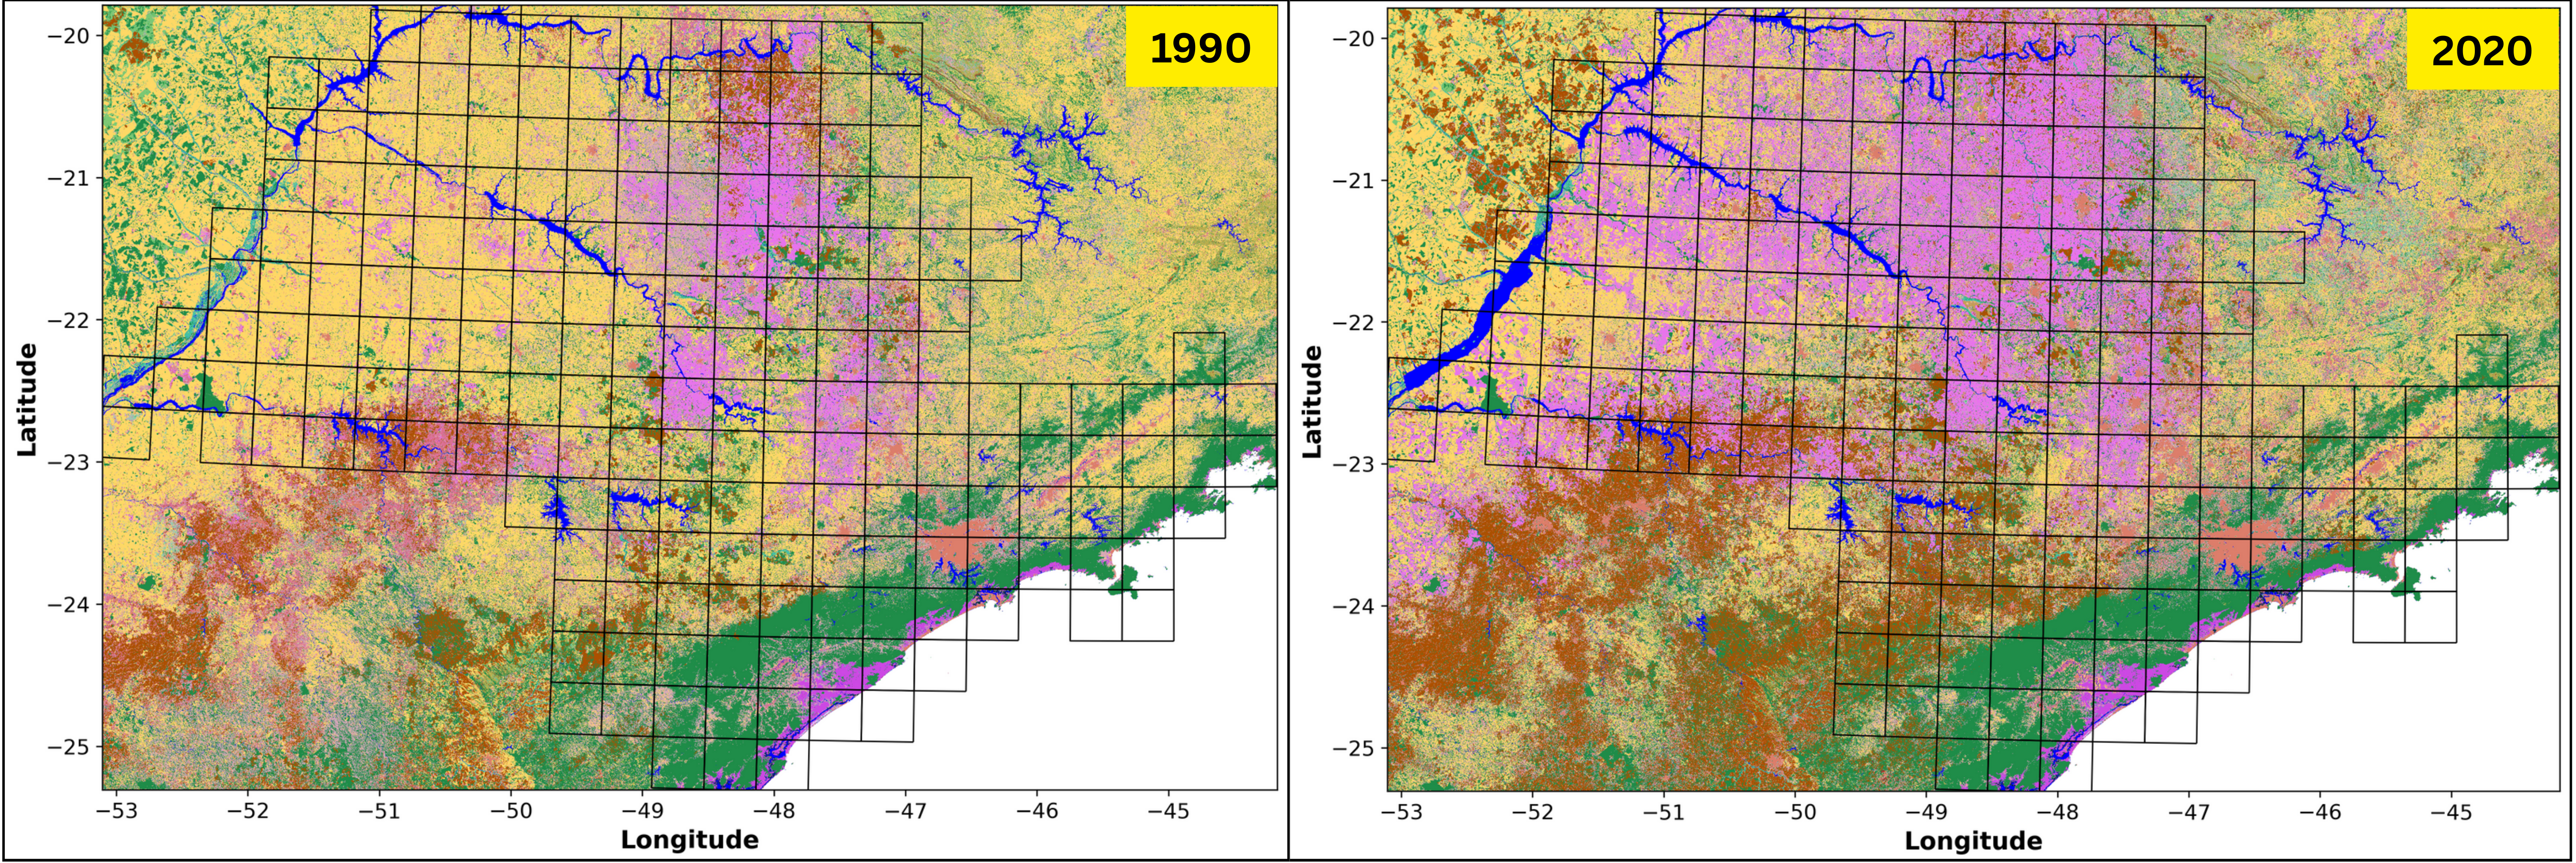
\includegraphics[width=1\textwidth]{fig/mapa_grade_sp.png}
\caption[Uso e cobertura da terra no estado de São Paulo em 1990 segundo classificação MapBiomas, Collection 9]{Uso e cobertura da terra no estado de São Paulo em 1990 segundo classificação MapBiomas, Collection 9. Observe a dominância de pastagens (tons amarelados), presença significativa de agricultura 
(tons rosados) e remanescentes de vegetação nativa (tons verdes) principalmente na Serra do Mar e Serra da Mantiqueira. Já ao lado direito o que temos é a relação do uso de cobertura da terra em 2020 segundo classificação, intensificação agrícola com redução de pastagens, e recuperação parcial de vegetação nativa em algumas áreas protegidas.}
\label{fig:mapbiomas_sp_1990}
\end{figure}

A Figura \ref{fig:mapbiomas_sp_1990} apresenta a distribuição espacial das classes de uso e cobertura da terra no estado de São Paulo em dois momentos distintos (1990 e 2020), evidenciando transformações substanciais ao longo do período de três décadas. Em 1990, o território paulista apresentava configuração caracterizada pela dominância de pastagens (tons amarelados) ocupando extensas áreas nas regiões centro, oeste e noroeste do estado, intercaladas com agricultura intensiva (tons rosados), particularmente concentrada no norte e noroeste. As formações florestais nativas (tons verdes escuros) encontravam-se predominantemente preservadas na Serra do Mar (faixa costeira sudeste) e em remanescentes dispersos na Serra da Mantiqueira (extremo leste). As áreas urbanizadas (tons avermelhados) já apresentavam expressão significativa na região metropolitana de São Paulo e em cidades médias do interior.

Já em 2020 o que se revela são transformações marcantes nesta configuração. Observa-se intensificação agrícola substancial, com expansão de cultivos de cana-de-açúcar (tons rosa-lilás) nas regiões norte, noroeste e centro-oeste, ocupando áreas anteriormente destinadas a pastagens. A conversão de pastagens de baixa produtividade em agricultura mecanizada é particularmente evidente nas regiões de Ribeirão Preto, Barretos e Araçatuba. Simultaneamente, as formações florestais na Serra do Mar e Serra da Mantiqueira apresentam aparente expansão ou adensamento (tons verdes mais intensos) \citep{sos_inpe_atlas_2023_2024}. A mancha urbana apresenta expansão moderada mas geograficamente concentrada, com crescimento mais visível na região metropolitana de São Paulo e no entorno de cidades médias do interior, representada pela intensificação dos tons avermelhados.

O estado do Rio Grande do Norte, por sua vez, apresenta transformações ainda mais dramáticas (Figura \ref{fig:mapbiomas_rn_1990}). As alterações observadas caracterizam um dos processos de conversão de vegetação nativa mais severos documentados no Brasil \citep{leal2003_caatinga, velloso2002_ecorregioes_caatinga}.

\begin{figure}[htbp]
\centering
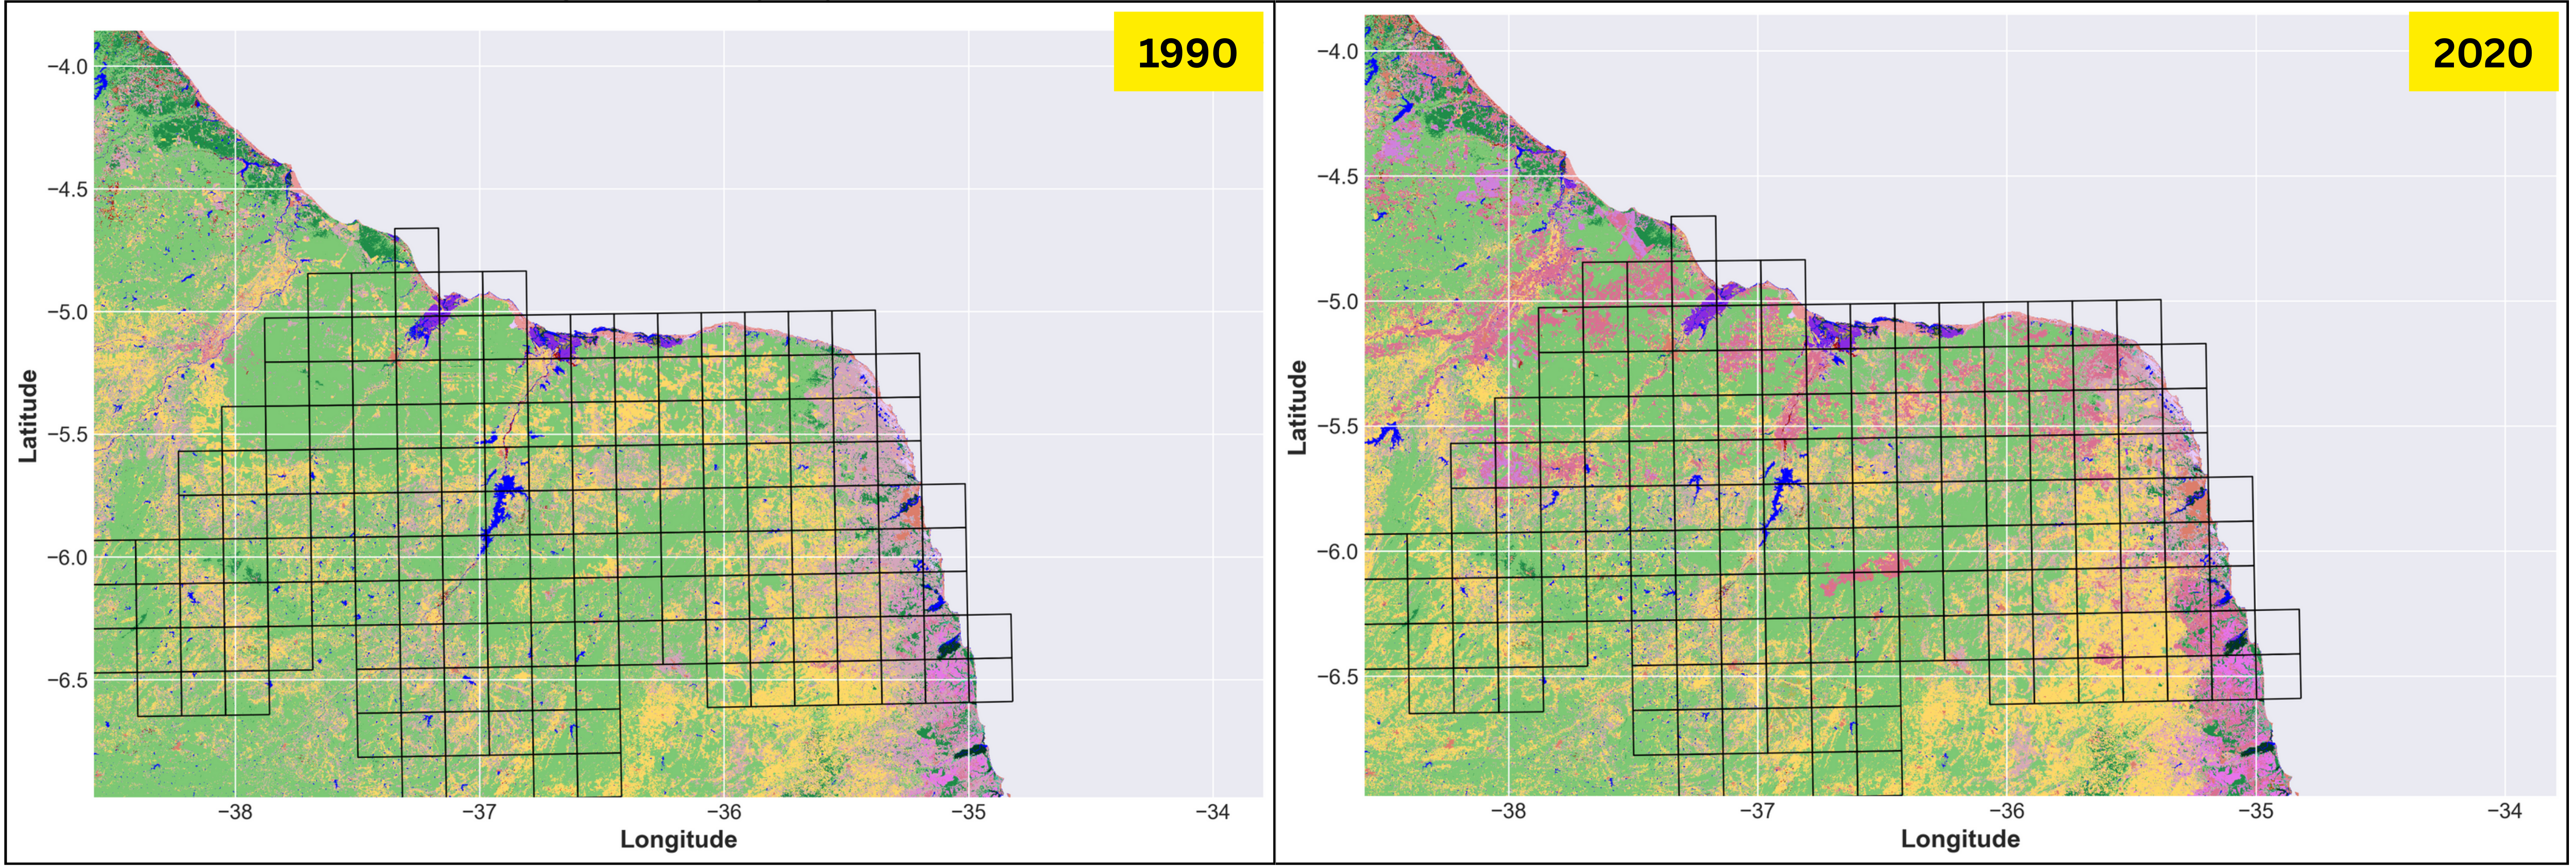
\includegraphics[width=1\textwidth]{fig/mapa_grade_rn.png}
\caption[Uso e cobertura da terra no estado do Rio Grande do Norte em 1990 segundo classificação MapBiomas, Collection 9]{Uso e cobertura da terra no estado do Rio Grande do Norte em 1990 segundo classificação MapBiomas, Collection 9. Observe a dominância de formação savânica (Caatinga) em tons verde-claro e verde-amarelado ocupando aproximadamente 79\% do território, refletindo extensão da vegetação 
nativa semiárida. A zona costeira apresenta manguezais (tons verde-escuro), aquicultura (tons lilás) e áreas urbanizadas. Já ao lado direito, em 2020, observa-se redução catastrófica da Caatinga (agora apenas 35,5\% do território), substituída principalmente por pastagens degradadas (tons amarelados), agricultura 
de sequeiro, solo exposto e áreas em diversos estágios de degradação ambiental.}
\label{fig:mapbiomas_rn_1990}
\end{figure}

A Figura \ref{fig:mapbiomas_rn_1990} apresenta a distribuição espacial das classes de uso e cobertura da terra no Rio Grande do Norte em 1990 e 2020. Em 1990, o estado apresentava dominância de formação savânica (Caatinga) representada em tons verde-claro e verde-amarelado, cobrindo aproximadamente 79\% do território e distribuída de forma relativamente contínua pelas regiões central, sul e oeste. A vegetação de Caatinga 
preservada era particularmente expressiva nas regiões do Seridó (centro-sul) e no interior semiárido, intercalada com manchas de pastagem (tons amarelados) e agricultura de sequeiro. A zona costeira já apresentava maior heterogeneidade, com presença de áreas urbanizadas concentradas em Natal e outras cidades litorâneas (tons avermelhados), atividades de aquicultura incipientes (tons lilás), manguezais preservados (tons verde-escuro) e agricultura irrigada em áreas específicas do litoral leste. Formações campestres e campos alagados (tons alaranjados e ciano) eram visíveis em áreas de transição ecológica e várzeas.

O painel de 2020 apresenta uma transformação particularmente drástica desta configuração original. A cobertura de Caatinga sofreu redução significativa e espacialmente generalizada, com conversão massiva em pastagens degradadas (tons amarelados agora predominantes em vastas áreas do interior), agricultura de sequeiro de baixa produtividade, solo exposto e áreas em diversos estágios de degradação ambiental 
\citep{santos2014caatinga, sudene2024desertificacao}. Esta conversão é particularmente severa e visualmente impactante nas regiões centro-norte e central do estado, onde a vegetação nativa característica (tons verdes) foi substituída quase completamente por tons amarelados. Os remanescentes de Caatinga preservada (tons verdes) restringem-se a fragmentos dispersos e áreas específicas no sul do estado e em localidades pontuais.

A região costeira apresenta expansão visível de áreas urbanizadas, especialmente em Natal, Mossoró e ao longo do litoral oriental (intensificação dos tons avermelhados), intensificação marcante da aquicultura com ampliação de manchas lilás. O contraste visual entre os dois painéis é extremamente marcante: o que em 1990 era um estado predominantemente coberto por vegetação nativa semiárida (tons verdes ocupando a maior 
parte do território) transformou-se em 2020 em território dominado por usos antrópicos de baixa produtividade e cobertura vegetal severamente degradada (tons amarelados).

\subsection{Análise das mudanças nas classes de uso da terra}

A quantificação das transformações no uso e cobertura da terra permite avaliar a magnitude absoluta e relativa das mudanças observadas nos mapas qualitativos apresentados anteriormente. As Figuras \ref{fig:sp_top10_classes} e \ref{fig:rn_top10_classes} apresentam as dez classes de uso da terra mais representativas em cada estado nos anos de 1990 e 2020, enquanto as Figuras \ref{fig:sp_variacao_classes} 
e \ref{fig:rn_variacao_classes} quantificam as variações absolutas (em pontos percentuais) experimentadas por cada classe ao longo do período de três décadas.

\subsubsection*{São Paulo: dinâmica das classes de uso da terra}

\begin{figure}[htbp]
\centering
\includegraphics[width=\textwidth]{fig/SP_top10_1990_2020.png}
\caption[Top 10 classes de uso do solo em São Paulo (1990 vs 2020)]{Top 10 classes de uso do solo em São Paulo para os anos de 1990 (azul) e 2020 (laranja). Observe a dramática redução de pastagens (de 37,4\% para 22,1\%) e o aumento correspondente de cana-de-açúcar (de 3,5\% para 12,1\%) e soja (de 0 para 8,1\%), refletindo intensificação agrícola generalizada.}
\label{fig:sp_top10_classes}
\end{figure}

A análise quantitativa para São Paulo (Figura \ref{fig:sp_top10_classes}) revela transformação profunda na estrutura de uso da terra. Em 1990, as pastagens dominavam o território do estado de São Paulo, ocupando 37,4\% da área total, seguidas por formação florestal (17,7\%) e mosaico de usos (13,9\%). Em 2020, embora as pastagens permaneçam como a classe mais representativa, sua extensão reduziu-se dramaticamente para 22,1\%, 
representando perda absoluta de 15,3 pontos percentuais. Esta redução massiva de pastagens foi compensada principalmente pela expansão de agricultura intensiva: cana-de-açúcar expandiu-se de 3,5\% para 12,1\%, soja de praticamente zero para 8,1\%, e formação campestre de 1,2\% para 4,3\%.

\begin{figure}[htbp]
\centering
\includegraphics[width=\textwidth]{fig/SP_variacao_top10_1990_2020.png}
\caption[Variação absoluta por classe de uso do solo em São Paulo (1990-2020)]
{Variação absoluta (em pontos percentuais) por classe de uso do solo em São Paulo entre 1990 e 2020. Cores vermelhas indicam redução; cores verdes indicam expansão. Destaque para a redução de $-15{,}3$\%. em pastagens e expansão de $+8{,}6\%$}
\label{fig:sp_variacao_classes}
\end{figure}

A Figura \ref{fig:sp_variacao_classes} quantifica estas transformações de forma ainda mais clara. A porcentagem indicada para a classe ``pastagens'' apresentam de longe a maior redução absoluta ($-15{,}3\%$), seguidas por "outras lavouras temporárias" ($-3{,}2\%$) e formação florestal ($-0{,}6\%$). Em contraste, cana-de-açúcar apresentou o maior ganho absoluto ($+8{,}6\%$), seguida por soja ($+4{,}8\%$) e formação campestre ($+3{,}1\%$). A formação florestal, embora tenha apresentado pequena redução em termos percentuais relativos ao território total estadual, manteve-se relativamente estável, variando de 17,7\% para 17,0\%, sugerindo que perdas florestais em algumas regiões foram parcialmente compensadas por recuperação em outras áreas, particularmente na Serra do Mar \citep{sos_inpe_atlas_2023_2024}.
\newpage
\subsubsection*{Rio Grande do Norte: dinâmica das classes de uso da terra}

\begin{figure}[htbp]
\centering
\includegraphics[width=\textwidth]{fig/RN_top10_1990_2020.png}
\caption[Top 10 classes de uso do solo no Rio Grande do Norte (1990 vs 2020)]
{Top 10 classes de uso do solo no Rio Grande do Norte para os anos de 1990 (azul) e 2020 (laranja). Observe a queda considerável da formação savânica (Caatinga), de 27,0\% para 23,6\%, e a expansão correspondente de pastagens (de 10,2\% para 11,4\%) e outras lavouras temporárias (de 0,2\% para 3,7\%).}
\label{fig:rn_top10_classes}
\end{figure}

A análise quantitativa para o Rio Grande do Norte (Figura \ref{fig:rn_top10_classes}) revela transformação ainda mais dramática que a observada em São Paulo, caracterizada pela diminuição da vegetação nativa de Caatinga. Em 1990, a formação savânica dominava o estado com 27,0\% do território, seguida por pastagens (10,2\%) e mosaico de usos (9,4\%). Em 2020, a formação savânica reduziu-se para 23,6\%, representando 
perda absoluta de 3,4 pontos percentuais da cobertura nativa. Simultaneamente, as pastagens expandiram-se moderadamente de 10,2\% para 11,4\% (+1,2\%), e particularmente notável foi a emergência de "outras lavouras temporárias" que expandiram dramaticamente de 0,2\% para 3,7\% (+3,5\%).

\begin{figure}[htbp]
\centering
\includegraphics[width=\textwidth]{fig/RN_variacao_top10_1990_2020.png}
\caption[Variação absoluta por classe de uso do solo no Rio Grande do Norte (1990-2020)]{Variação absoluta (em pontos percentuais) por classe de uso do solo no Rio Grande do Norte entre 1990 e 2020. Cores vermelhas indicam redução; cores verdes indicam expansão. Destaque para a redução de $-3{,}4$\%. em formação savânica (Caatinga) e $-2{,}3$\%. em mosaico de usos, substituídos principalmente por outras lavouras temporárias ($+3{,}5$\%) e pastagens ($+1{,}2$\%).}
\label{fig:rn_variacao_classes}
\end{figure}

A Figura \ref{fig:rn_variacao_classes} quantifica estas transformações de forma detalhada. A formação savânica (Caatinga) apresentou a maior redução absoluta ($-3{,}4$\%), seguida por mosaico de usos ($-2{,}3$\%) e formação florestal ($-0{,}3$\%). Em contraste, "outras lavouras temporárias" apresentaram o maior ganho absoluto ($+3{,}5$\%), seguidas por pastagens ($+1{,}2$\%), outras lavouras perenes ($+0{,}9$\%) e área urbanizada ($+0{,}6$\%). O padrão geral indica processo de conversão extensiva de vegetação nativa de Caatinga em usos antrópicos de baixa produtividade, particularmente pastagens degradadas e agricultura 
de sequeiro, caracterizando um dos processos de degradação ambiental mais severos documentados no semiárido brasileiro \citep{leal2003_caatinga, sudene2024desertificacao}.

\subsection{Avaliação e extremos de cobertura de solo no estado de São Paulo}

\begin{figure}[htbp]
\centering
\includegraphics[width=1\textwidth]{fig/mapa_blocos_extremos_sp.png}
\caption[Áreas de maior e menor mudança de formação florestal em percentis]{Áreas de maior e menor mudança de formação florestal em percentis, onde a maior perda (desmatamento) está em destaque com tons avermelhados, a menor perda ou cobertura constante em tons amarelados, já o ganho de área florestal está representada em tons de verde.}
\label{fig:mapa_blocos_extremos_sp}
\end{figure}

Ao analisar a Figura \ref{fig:mapa_blocos_extremos_sp} o que se destacam são: A evolução temporal da cobertura de formação florestal (predominantemente Mata Atlântica) apresenta duas trajetórias distintas que refletem diferentes contextos espaciais. Em áreas sob maior pressão de conversão agrícola e urbana, a cobertura florestal reduziu-se de 15,0\% em 1990 para 6,0\% em 2020, representando perda absoluta de 9,0 pontos percentuais. 

Avaliando progressivamente o comportamento de 10 em 10 anos, o que se observa é uma queda progressiva nos últimos anos, estabilizando-se de 2010 à 2020, Figura \ref{fig:evolucao_cobertura_sp}.

\begin{figure}[htbp]
\centering
\includegraphics[width=\textwidth]{fig/evolucao_cobertura_vegetal_sp.png}
\caption{Evolução temporal da cobertura de formação florestal no estado de São Paulo (1990-2020). Linha vermelha sólida (Perda \#1, Cell 3) e tracejada (Perda \#2, Cell 146) representam células com maior perda de cobertura florestal; linhas verdes sólida (Ganho \#1, Cell 93) e tracejada (Ganho \#2, Cell 78) representam células com ganho ou preservação de cobertura florestal.}
\label{fig:evolucao_cobertura_sp}
\end{figure}

Em contraste, a linha verde representa áreas com trajetória oposta, iniciando em 40,3\% de cobertura florestal em 1990 e apresentando crescimento progressivo para 45,0\% (2000), 47,0\% (2010) e 49,8\% (2020), totalizando ganho de 9,5 pontos percentuais ao longo do período.

A análise integrada das duas figuras evidencia portanto que as mudanças na cobertura florestal paulista não seguem padrão estadual homogêneo. As perdas concentram-se em regiões de agricultura intensiva no interior (noroeste), enquanto ganhos ocorrem em áreas de proteção ambiental e topografia acidentada (Serra do Mar) 
\citep{sos_inpe_atlas_2023_2024}.

\subsection{Avaliação e extremos de cobertura de solo no estado do Rio Grande do Norte}

A análise espacial (Figura \ref{fig:mapa_blocos_extremos_rn}) revela alta heterogeneidade, com células individuais apresentando perdas de até $-43{,}4\%$ e ganhos de até $+14{,}0\%$ de cobertura de Caatinga entre 1990 e 2020. O mapa evidencia padrão espacial complexo: áreas de maior perda (tons vermelho-escuro) concentram-se predominantemente na região centro-norte do estado (célula com perda máxima de $-43{,}4\%$ localizada em latitude $-5^\circ$ e longitude $-37^\circ$, correspondendo aproximadamente à região do Seridó), enquanto áreas de ganho ou menor mudança (tons verdes) distribuem-se principalmente no sul e sudoeste (célula com ganho máximo de $+14{,}0\%$ em latitude $-6{,}5^\circ$ e longitude $-38^\circ$). A região central e leste apresenta mosaico heterogêneo de perdas moderadas a severas (tons alaranjados a vermelhos).

\begin{figure}[htbp]
	\centering
	\includegraphics[width=\textwidth]{fig/mapa_blocos_extremos_rn.png}
	\caption[Distribuição espacial das mudanças na cobertura de formação savânica (Caatinga) no Rio Grande do Norte (1990-2020)]{Distribuição espacial das mudanças na cobertura de formação savânica (Caatinga) no Rio Grande do Norte (1990-2020) por célula de 100×100 km. Tons vermelhos indicam maior perda (desmatamento); tons amarelados representam mudanças moderadas; tons verdes indicam ganho ou estabilidade.}
	\label{fig:mapa_blocos_extremos_rn}
\end{figure}

A Figura \ref{fig:evolucao_cobertura_rn} revela as trajetórias temporais que caracterizam estas regiões extremas. A linha vermelha representa áreas sob maior pressão antrópica, onde a cobertura de Caatinga sofreu redução de 79,0\% em 1990 para aproximadamente 68,0\% em 2000, seguida por nova queda para 60,0\% em 2010, decaindo progressivamente para 35,5\% em 2020. Esta trajetória evidencia processo de degradação acelerada, particularmente severa na última década (2010-2020), quando ocorreu a maior taxa absoluta de perda ($-24{,}5\%$ em apenas 10 anos).

\begin{figure}[htbp]
	\centering
	\includegraphics[width=\textwidth]{fig/evolucao_cobertura_vegetal_rn.png}
	\caption[Evolução temporal da cobertura de formação savânica (Caatinga) no Rio Grande do Norte (1990-2020)]{Evolução temporal da cobertura de formação savânica (Caatinga) no Rio Grande do Norte (1990-2020). Linha vermelha representa células com maior perda de cobertura; linha verde representa células com menor mudança ou recuperação.}
	\label{fig:evolucao_cobertura_rn}
\end{figure}

Em contraste marcante, a linha verde representa áreas com trajetória de recuperação ou preservação relativa, iniciando em 56,6\% de cobertura em 1990 e apresentando crescimento progressivo para 62,0\% (2000), 73,0\% (2010), com leve redução para 70,6\% (2020), resultando em ganho de 14{,}0\% ao longo do período. Passando para o processo de diminuição, linhas vermelha, é observado um decaimento considerável da perda savânica após 2010 (linha vermelha: queda de 60\% para 35,5\%) contrasta com relativa estabilização nas áreas menos degradadas (linha verde: pequena redução de 73\% para 70,6\%).

A análise integrada das duas figuras evidencia que o Rio Grande do Norte experimenta processo de diferenciação espacial extrema, com áreas apresentando um comportamento e recuperação de cobertura vegetal, enquanto a maioria do território sofre degradação progressiva quando observado em conjunto com a Figura \ref{fig:mapa_blocos_extremos_rn} que demonstra uma mudança considerável nos dois cenários.

\section{Variáveis climáticas em áreas de extremos de mudança de cobertura}

A análise das variáveis climáticas em blocos de grade apresentadas no decorrer desta seção pelas Figuras \ref{fig:mapa_blocos_extremos_sp} e \ref{fig:mapa_blocos_extremos_rn} com a descrição das localidades das mudanças extremas de mudança de cobertura vegetal, permite avaliar se as variações de cobertura estão associadas aos padrões climáticos analisados nas seções anteriores. Para cada estado, selecionaram-se quatro blocos representando os extremos: os dois blocos com maior perda de vegetação nativa versus os dois blocos com maior ganho ou menor perda de vegetação. As médias anuais de temperatura e radiação solar e acumulados de precipitação foram calculadas para estes quatro blocos ao longo do período 1990--2024.

\subsection{São Paulo: Formação Florestal}

\subsubsection*{Temperatura}

A Figura \ref{fig:temp_extremos_sp} apresenta as médias anuais de temperatura para os quatro blocos extremos de mudança de formação florestal no estado de São Paulo. Observa-se clara e persistente separação térmica entre os dois grupos ao longo de todo o período analisado. Os dois blocos com maior perda de vegetação florestal (linhas vermelhas, sólida e tracejada) apresentam temperaturas consistentemente elevadas, oscilando entre 24,0 e 26,5°C ao longo da série temporal, com média aproximada de 24,8°C. Em contraste marcante, os dois blocos com ganho ou menor perda florestal (linhas verdes, sólida e tracejada) mantêm-se consistentemente mais frios, variando entre 17,5 e 20,5°C, com média próxima a 19,0°C.

\begin{figure}[htbp]
	\centering
	\includegraphics[width=\textwidth]{fig/temp_formacao_florestal_sp.png}
	\caption{Médias anuais de temperatura (°C) em quatro blocos extremos de mudança de formação florestal em São Paulo (1990--2024). Linhas vermelhas: blocos com maior perda florestal. Linhas verdes: blocos com ganho ou menor perda florestal.}
	\label{fig:temp_extremos_sp}
\end{figure}

A diferença entre os dois grupos mantém-se notavelmente constante em aproximadamente 5,0 a 5,5°C ao longo de três décadas e meia. As trajetórias histórica dos dois blocos de cada grupo apresentam comportamento coerente entre si, com as linhas vermelhas (Perda \#1 e Perda \#2) seguindo trajetórias praticamente paralelas, assim como as linhas verdes (Ganho \#1 e Ganho \#2), reforçando o padrão observado. Esta magnitude e persistência da diferença térmica sugerem que ela é primariamente determinada por fatores geográficos (altitude, latitude) \citep{alvares2013}, ao invés de mudanças dinâmicas na cobertura vegetal. Os blocos com maior perda florestal localizam-se predominantemente no interior noroeste do estado, em altitudes baixas (300--500m) e latitudes menores, enquanto blocos com ganho ou menor perda concentram-se na Serra do Mar, em altitudes elevadas (800--1200m) e latitude ligeiramente maior.

Ambos os grupos apresentam tendência clara de aquecimento ao longo do período, particularmente visível após 2010. Blocos com maior perda florestal mostram aquecimento de aproximadamente 1,5 a 2,0°C entre 1990 e 2024, enquanto blocos preservados apresentam aquecimento de magnitude similar (1,0 a 1,5°C). A consistência das taxas de aquecimento entre os dois grupos, independentemente da magnitude da mudança de cobertura florestal, sugere que o aquecimento regional é controlado primariamente por forçantes climáticas de grande escala \citep{ipcc2021} ao invés de mudanças locais na cobertura vegetal.

\subsubsection*{Radiação Solar}

A Figura \ref{fig:rad_extremos_sp} evidencia comportamento de radiação solar incidente fundamentalmente distinto entre os dois grupos de blocos. Os dois blocos com maior perda florestal (linhas vermelhas) apresentam valores consistentemente elevados e trajetórias altamente coerentes entre si, oscilando entre 205 e 238~W/m$^2$ ao longo da série temporal, com média aproximada de 220~W/m$^2$. Os dois blocos preservados (linhas verdes) mantêm radiação substancialmente inferior, também com alta coerência interna, variando entre 170 e 220~W/m$^2$, com média próxima a 190~W/m$^2$.

\begin{figure}[htbp]
	\centering
	\includegraphics[width=\textwidth]{fig/rad_formacao_florestal_sp.png}
	\caption{Médias anuais de radiação solar incidente (W/m$^2$) em quatro blocos extremos de mudança de formação florestal em São Paulo (1990--2024). Linhas vermelhas: blocos com maior perda florestal. Linhas verdes: blocos com ganho ou menor perda florestal.}
	\label{fig:rad_extremos_sp}
\end{figure}

A diferença radiativa entre os grupos permanece aproximadamente constante em 30 a 40~W/m$^2$ ao longo do período, representando redução de cerca de 15 a 20\% na radiação disponível nas áreas preservadas comparadas às áreas com maior perda florestal. A alta coerência temporal entre os dois blocos de cada grupo (linhas praticamente paralelas dentro de cada cor) demonstra que esta diferença é geograficamente determinada e persistente. Regiões preservadas na Serra do Mar apresentam maior nebulosidade orográfica devido ao levantamento de massas de ar úmidas oceânicas, enquanto blocos do interior noroeste beneficiam-se de maior transparência atmosférica e menor nebulosidade média, resultando em maior incidência de radiação sobre a superfície \citep{yamasoe2017}.

Ambos os grupos apresentam tendência de aumento da radiação solar ao longo do período, particularmente evidente após 2015. A taxa de aumento é similar entre os grupos (aproximadamente 15 a 20~W/m$^2$ ao longo de 34 anos), com ambas as linhas de cada grupo seguindo trajetórias ascendentes paralelas, sugerindo que esta tendência de brightening \citep{wild2012} é controlada por processos atmosféricos regionais ao invés de mudanças locais na cobertura vegetal.

\subsubsection*{Precipitação}

A Figura \ref{fig:prec_extremos_sp} apresenta diferenças marcantes de precipitação acumulada entre os dois grupos de blocos. Os dois blocos com ganho ou menor perda florestal (linhas verdes), localizados predominantemente na Serra do Mar, apresentam precipitação acumulada anual consistentemente superior e trajetórias altamente coerentes entre si, oscilando entre 60.000 e 110.000~mm acumulados, com média próxima a 85.000~mm. Em contraste, os dois blocos com maior perda florestal (linhas vermelhas), situados no interior noroeste, apresentam valores substancialmente inferiores e também alta coerência interna, variando entre 50.000 e 80.000~mm, com média próxima a 65.000~mm.

\begin{figure}[htbp]
	\centering
	\includegraphics[width=\textwidth]{fig/prec_formacao_florestal_sp.png}
	\caption[Precipitação total anual (mm) em quatro blocos extremos de mudança de formação florestal em São Paulo (1990--2024)]{Precipitação total anual (mm) em quatro blocos extremos de mudança de formação florestal em São Paulo (1990--2024). Valores representam acumulados totais considerando a área dos blocos de grade. Linhas vermelhas: blocos com maior perda florestal. Linhas verdes: blocos com ganho ou menor perda florestal.}
	\label{fig:prec_extremos_sp}
\end{figure}

A diferença de precipitação entre os grupos mantém-se relativamente constante ao longo do período, oscilando entre 15.000 e 30.000~mm dependendo do ano específico, equivalente a aproximadamente 20 a 35\% a mais de precipitação nas áreas preservadas. A alta coerência entre os dois blocos de cada grupo (trajetórias praticamente paralelas dentro de cada cor) demonstra que esta diferença é novamente geograficamente determinada. Esta diferença é controlada por efeitos como: blocos preservados na Serra do Mar beneficiam-se de intensificação pluviométrica devido ao levantamento forçado de massas de ar úmidas oceânicas que ascendem as encostas da serra, experimentam resfriamento adiabático, condensação e precipitação intensificada, particularmente nas vertentes voltadas para o oceano \citep{nimer1989, alvares2013}.

Observa-se tendência sutil de redução de precipitação em ambos os grupos após 2015, com os blocos de maior perda florestal apresentando declínio ligeiramente mais significativo. Porém, a interpretação destas diferenças de precipitação requer um aprofundamento na análise: embora blocos preservados recebam substancialmente mais precipitação, esta diferença reflete primariamente localização geográfica (Serra do Mar versus interior) ao invés de efeitos diretos da cobertura vegetal \citep{li2015local}. As mesmas características topográficas que induzem alta precipitação também favoreceram historicamente a preservação florestal, criando correlação geográfica que não implica necessariamente causalidade. Efeitos da vegetação sobre precipitação local através de evapotranspiração e ciclagem de umidade \citep{eagleson1978, Trenberth2009} podem existir.

\subsection{Rio Grande do Norte: Formação Savânica}

\subsubsection*{Temperatura}

A Figura \ref{fig:temp_extremos_rn} apresenta as médias anuais de temperatura para os quatro blocos extremos de mudança de Caatinga no Rio Grande do Norte. Em contraste marcante com São Paulo, observa-se que os quatro blocos apresentam temperaturas altamente convergentes ao longo de todo o período analisado, com as quatro linhas frequentemente entrelaçadas e sobrepondo-se umas às outras. Os dois blocos com maior redução de Caatinga (linhas vermelhas) oscilam entre 27,0 e 29,2°C, enquanto os dois blocos com ganho ou menor redução (linhas verdes) variam entre 27,0 e 28,5°C, com todas as quatro linhas convergindo repetidamente ao longo da série temporal.

\begin{figure}[htbp]
	\centering
	\includegraphics[width=\textwidth]{fig/temp_formacao_savânica_rn.png}
	\caption{Médias anuais de temperatura (°C) em quatro blocos extremos de mudança de formação savânica (Caatinga) no Rio Grande do Norte (1990--2024). Linhas vermelhas: blocos com maior perda de Caatinga. Linhas verdes: blocos com ganho ou menor perda de Caatinga.}
	\label{fig:temp_extremos_rn}
\end{figure}

A diferença térmica média entre os grupos é mínima, tipicamente inferior a 0,5°C, e não apresenta consistência temporal. A ausência de diferenciação clara entre os quatro blocos, independentemente da magnitude da mudança de cobertura vegetal, contrasta fortemente com o padrão observado em São Paulo. A variabilidade interanual supera amplamente qualquer possível diferença sistemática entre áreas preservadas e degradadas, dificultando na identificação de sinais associados especificamente a mudanças na cobertura de Caatinga. A análise visual sugere possível tendência sutil de aquecimento ao longo do período em todos os blocos, consistente com tendências regionais apresentadas anteriormente \citep{santos2014caatinga}, mas sem diferença detectável nas taxas de aquecimento entre blocos preservados e degradados.

\subsubsection*{Radiação Solar}

A Figura \ref{fig:rad_extremos_rn} apresenta padrão notavelmente distinto daquele observado em São Paulo. Os quatro blocos (dois de maior perda de Caatinga em vermelho e dois de ganho ou menor perda em verde) apresentam valores de radiação solar altamente convergentes, com as quatro linhas entrelaçando-se e sobrepondo-se substancialmente ao longo da série temporal. Todos os blocos oscilam em faixas que se sobrepõem amplamente, variando entre aproximadamente 245 e 277~W/m$^2$, sem diferença sistemática consistente entre blocos de perda e blocos de ganho.

\begin{figure}[htbp]
	\centering
	\includegraphics[width=\textwidth]{fig/rad_formação_savânica_rn.png}
	\caption{Médias anuais de radiação solar incidente (W/m$^2$) em quatro blocos extremos de mudança de formação savânica (Caatinga) no Rio Grande do Norte (1990--2024). Linhas vermelhas: blocos com maior perda de Caatinga. Linhas verdes: blocos com ganho ou menor perda de Caatinga.}
	\label{fig:rad_extremos_rn}
\end{figure}

A alta variabilidade interanual observada em todos os blocos (oscilações de até 30 a 35~W/m$^2$ entre anos consecutivos) supera amplamente qualquer diferença média potencial entre os grupos, dificultando a identificação de sinais associados especificamente a mudanças na cobertura vegetal \citep{alkama2016biophysical, duveiller2018local}. O entrelaçamento constante das quatro linhas ao longo de toda a série temporal demonstra que blocos com históricos radicalmente distintos de mudança de cobertura (perda severa versus ganho substancial) experimentam condições radiativas essencialmente indistinguíveis. Esta variabilidade está provavelmente associada a flutuações na nebulosidade durante a estação chuvosa \citep{medeiros2017}, que varia de ano para ano dependendo da intensidade e posicionamento da Zona de Convergência Intertropical \citep{kousky1980diurnal}.

\subsubsection*{Precipitação}

A Figura \ref{fig:prec_extremos_rn} apresenta o comportamento da precipitação acumulada com características específicas do semiárido. Os quatro blocos apresentam precipitação total anual variando entre aproximadamente 3.000 e 30.000~mm, com variabilidade interanual extremamente elevada que domina completamente qualquer diferença média potencial entre os grupos. As quatro linhas entrelaçam-se de forma consistente ao longo da série, com alternância frequente de posições entre blocos de perda e blocos de ganho.

\begin{figure}[htbp]
	\centering
	\includegraphics[width=\textwidth]{fig/prec_formação_savânica_rn.png}
	\caption{Precipitação total anual (mm) em quatro blocos extremos de mudança de formação savânica (Caatinga) no Rio Grande do Norte (1990--2024). Linhas vermelhas: blocos com maior perda de Caatinga. Linhas verdes: blocos com ganho ou menor perda de Caatinga.}
	\label{fig:prec_extremos_rn}
\end{figure}

O coeficiente de variação interanual para todos os blocos excede 60\%, valor altos mesmo para padrões semiáridos \citep{marengo2017drought, marengo2017}. Eventos de seca severa (precipitação $<$5.000~mm) alternam-se com anos relativamente úmidos ($>$25.000~mm) sem padrão previsível. Esta alta variabilidade dificulta a identificação de possíveis diferenças entre áreas preservadas e degradadas.

Os dois blocos com ganho ou menor perda de Caatinga (linhas verdes) apresentam tendência sutil de precipitação ligeiramente superior em alguns anos, particularmente visível nos picos de 2011 (~30.000~mm) e 2024 (~26.000~mm). No entanto, esta diferença não é consistente ao longo da série e pode refletir simplesmente localização geográfica dos blocos (sul do estado tipicamente recebe precipitação ligeiramente superior devido à maior influência de sistemas frontais) \citep{velloso2002_ecorregioes_caatinga} ao invés de efeitos diretos da cobertura vegetal. A convergência frequente das quatro linhas em anos secos (particularmente 2012--2013 e 2016--2017) demonstra que em condições de seca severa, controlada por circulação atmosférica de grande escala, possíveis efeitos locais da vegetação tornam-se irrelevantes.

\subsection{Evolução espaciotemporal das variáveis climáticas e uso da terra}

As Figuras \ref{fig:mapas_temporais_rn} e \ref{fig:mapas_temporais_sp} apresentam a evolução espacial simultânea de uso da terra e variáveis climáticas em intervalos decadais (1990, 2000, 2010, 2020), permitindo avaliação visual de possíveis associações entre transformações de cobertura vegetal e mudanças climáticas localizadas.


\subsubsection*{São Paulo}

\begin{figure}[H]
	\centering
	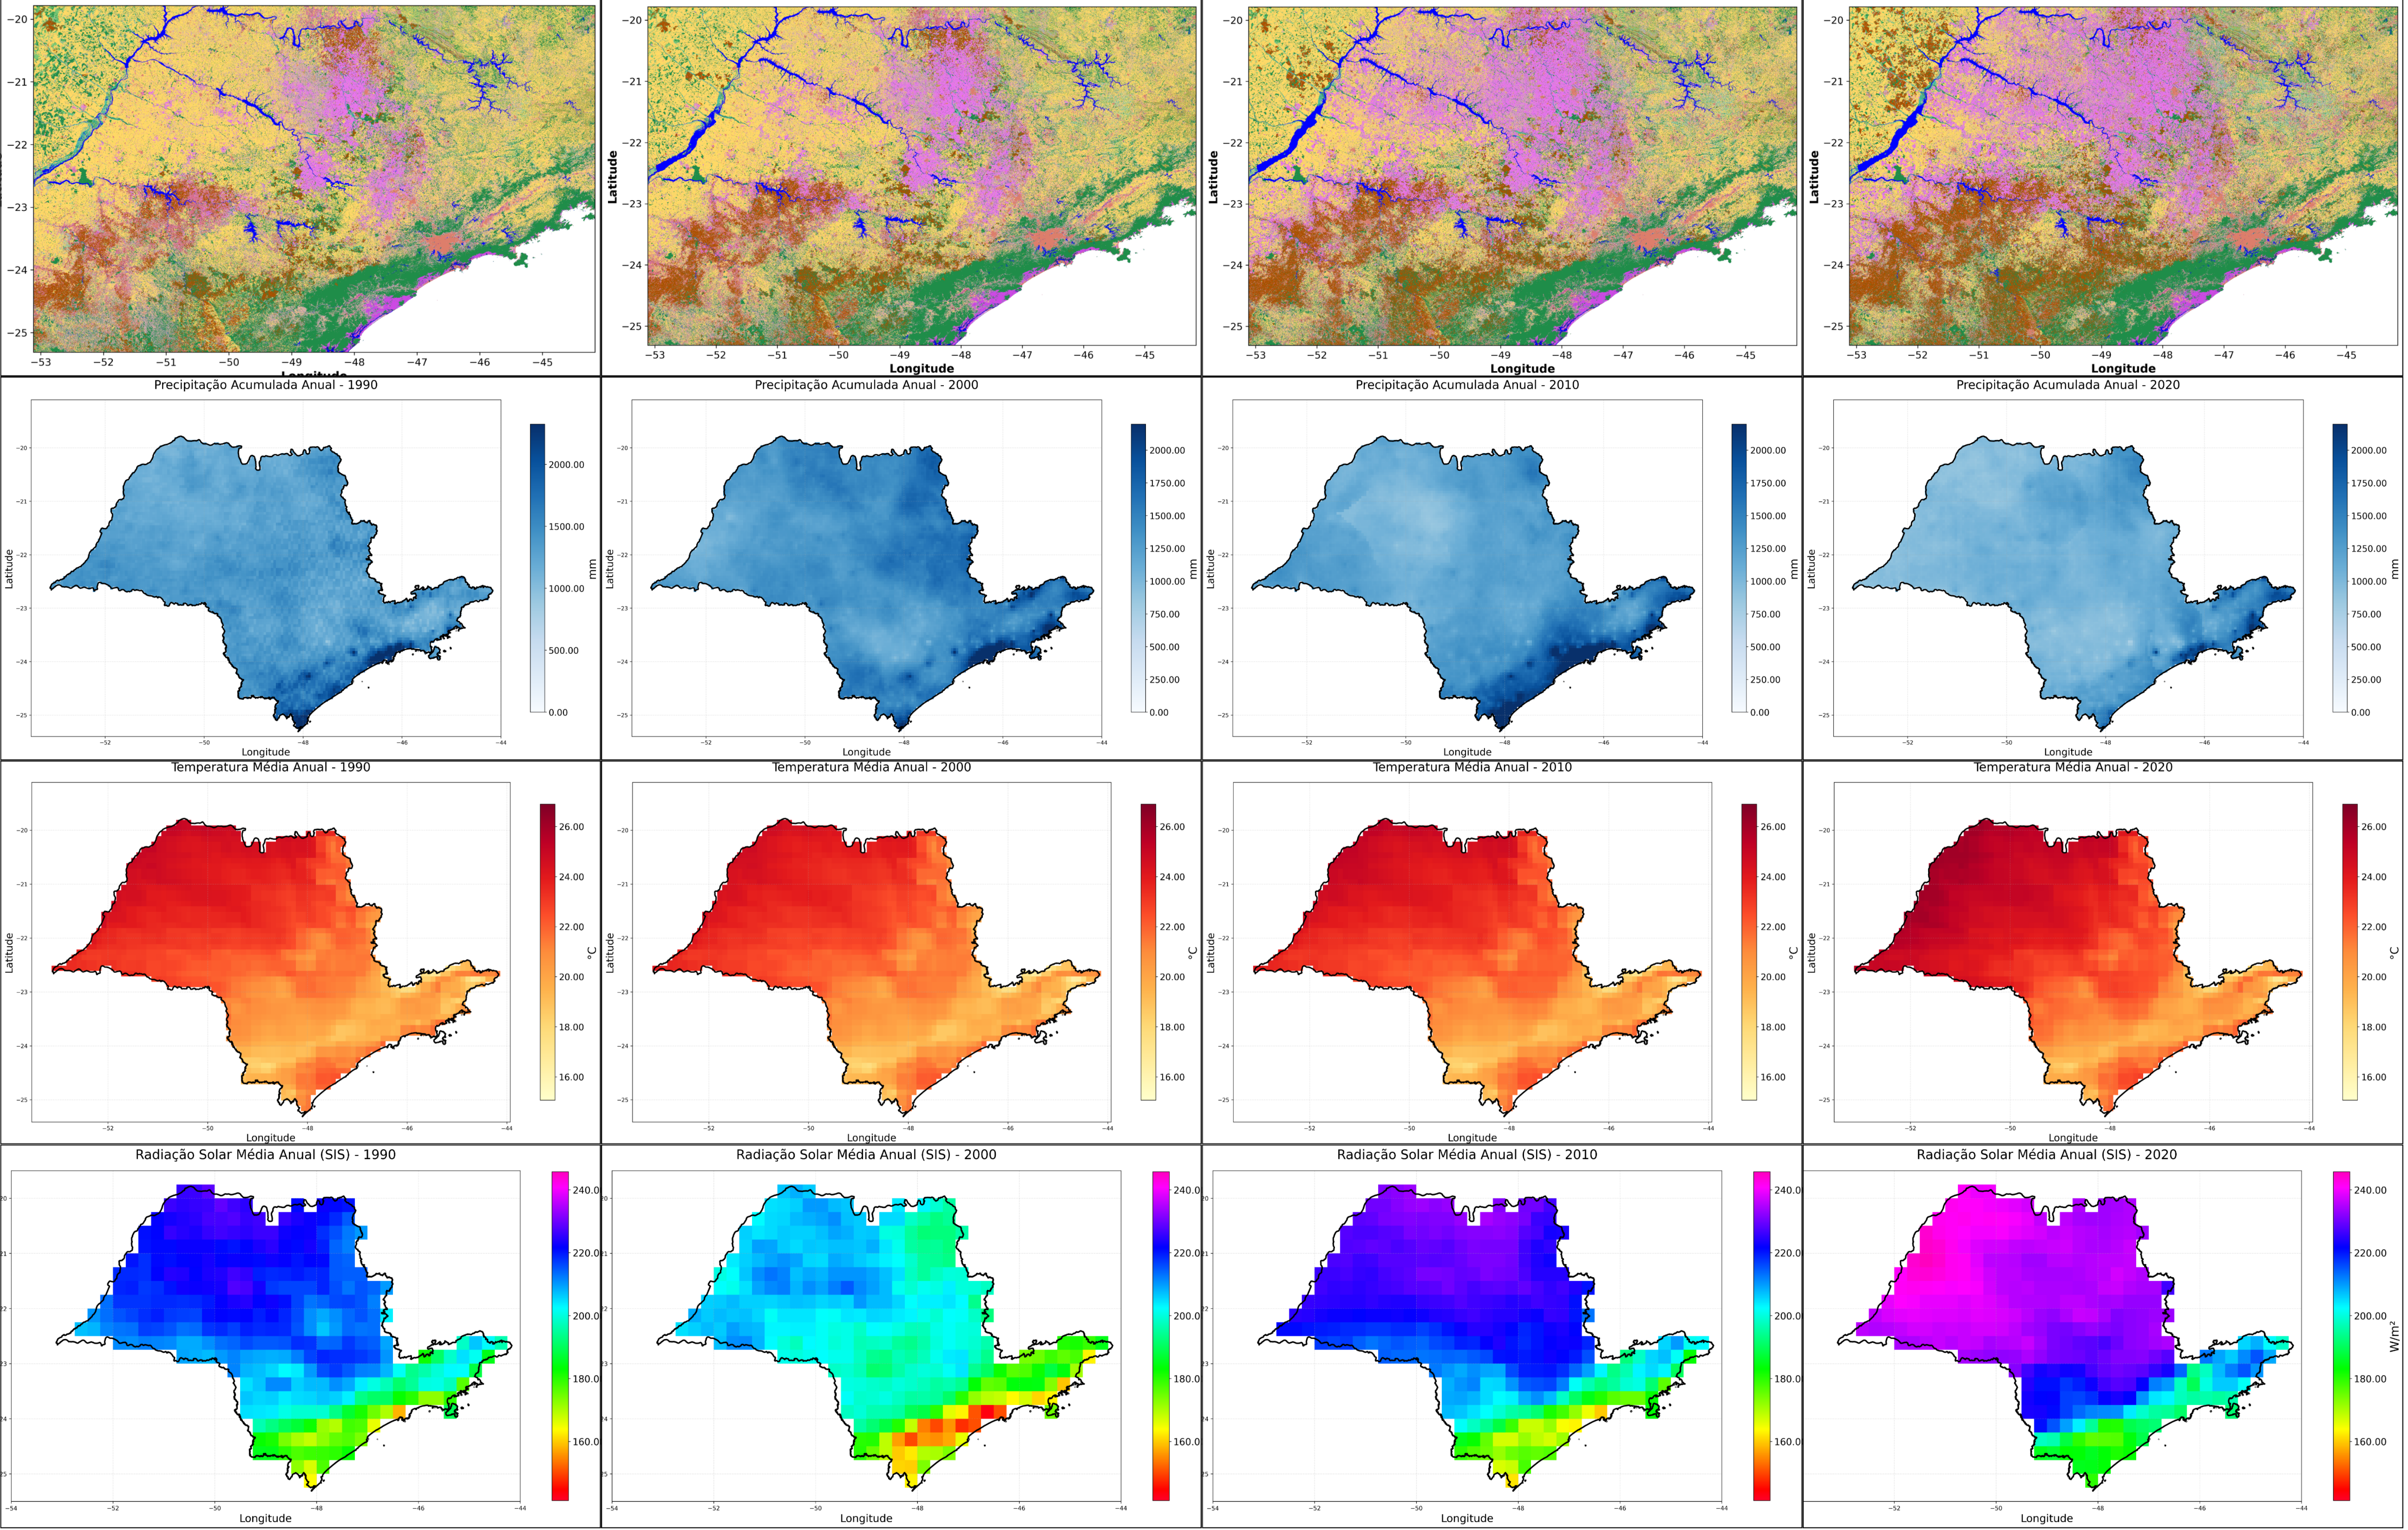
\includegraphics[width=\textwidth]{fig/mapas_sp.png}
	\caption[Evolução temporal do uso da terra - SP]{Evolução temporal do uso da terra (linha superior), precipitação acumulada anual (segunda linha), temperatura média anual (terceira linha) e radiação solar média anual (linha inferior) em São Paulo para os anos de 1990, 2000, 2010 e 2020.}
	\label{fig:mapas_temporais_sp}
\end{figure}

A linha superior da Figura \ref{fig:mapas_temporais_sp} descreve a transformação agrícola progressiva. Entre 1990 e 2020, observa-se conversão substancial de pastagens (tons amarelados) em agricultura intensiva (tons rosa-lilás) nas regiões norte, noroeste e central do estado. Simultaneamente, a Serra do Mar mantém ou intensifica tonalidade verde, consistente com preservação ou recuperação de cobertura florestal.

As variáveis climáticas (linhas 2-4) mantêm padrões espaciais notavelmente estáveis ao longo dos 30 anos. A precipitação preserva gradiente litoral-interior característico em todos os períodos. A temperatura mostra gradiente topográfico estável (Serra do Mar mais fria, interior mais quente) que se mantém praticamente inalterado apesar das transformações de uso da terra.

A radiação solar mantém padrão inverso ao da precipitação (máximos no interior, mínimos no litoral) de forma consistente nos quatro períodos. A estabilidade deste padrão ao longo de três décadas de intensas mudanças agrícolas sugere que nebulosidade, determinada primariamente por topografia e circulação atmosférica de grande escala, domina sobre possíveis efeitos da vegetação sobre radiação.

\subsubsection*{Rio Grande do Norte}

\begin{figure}[H]
	\centering
	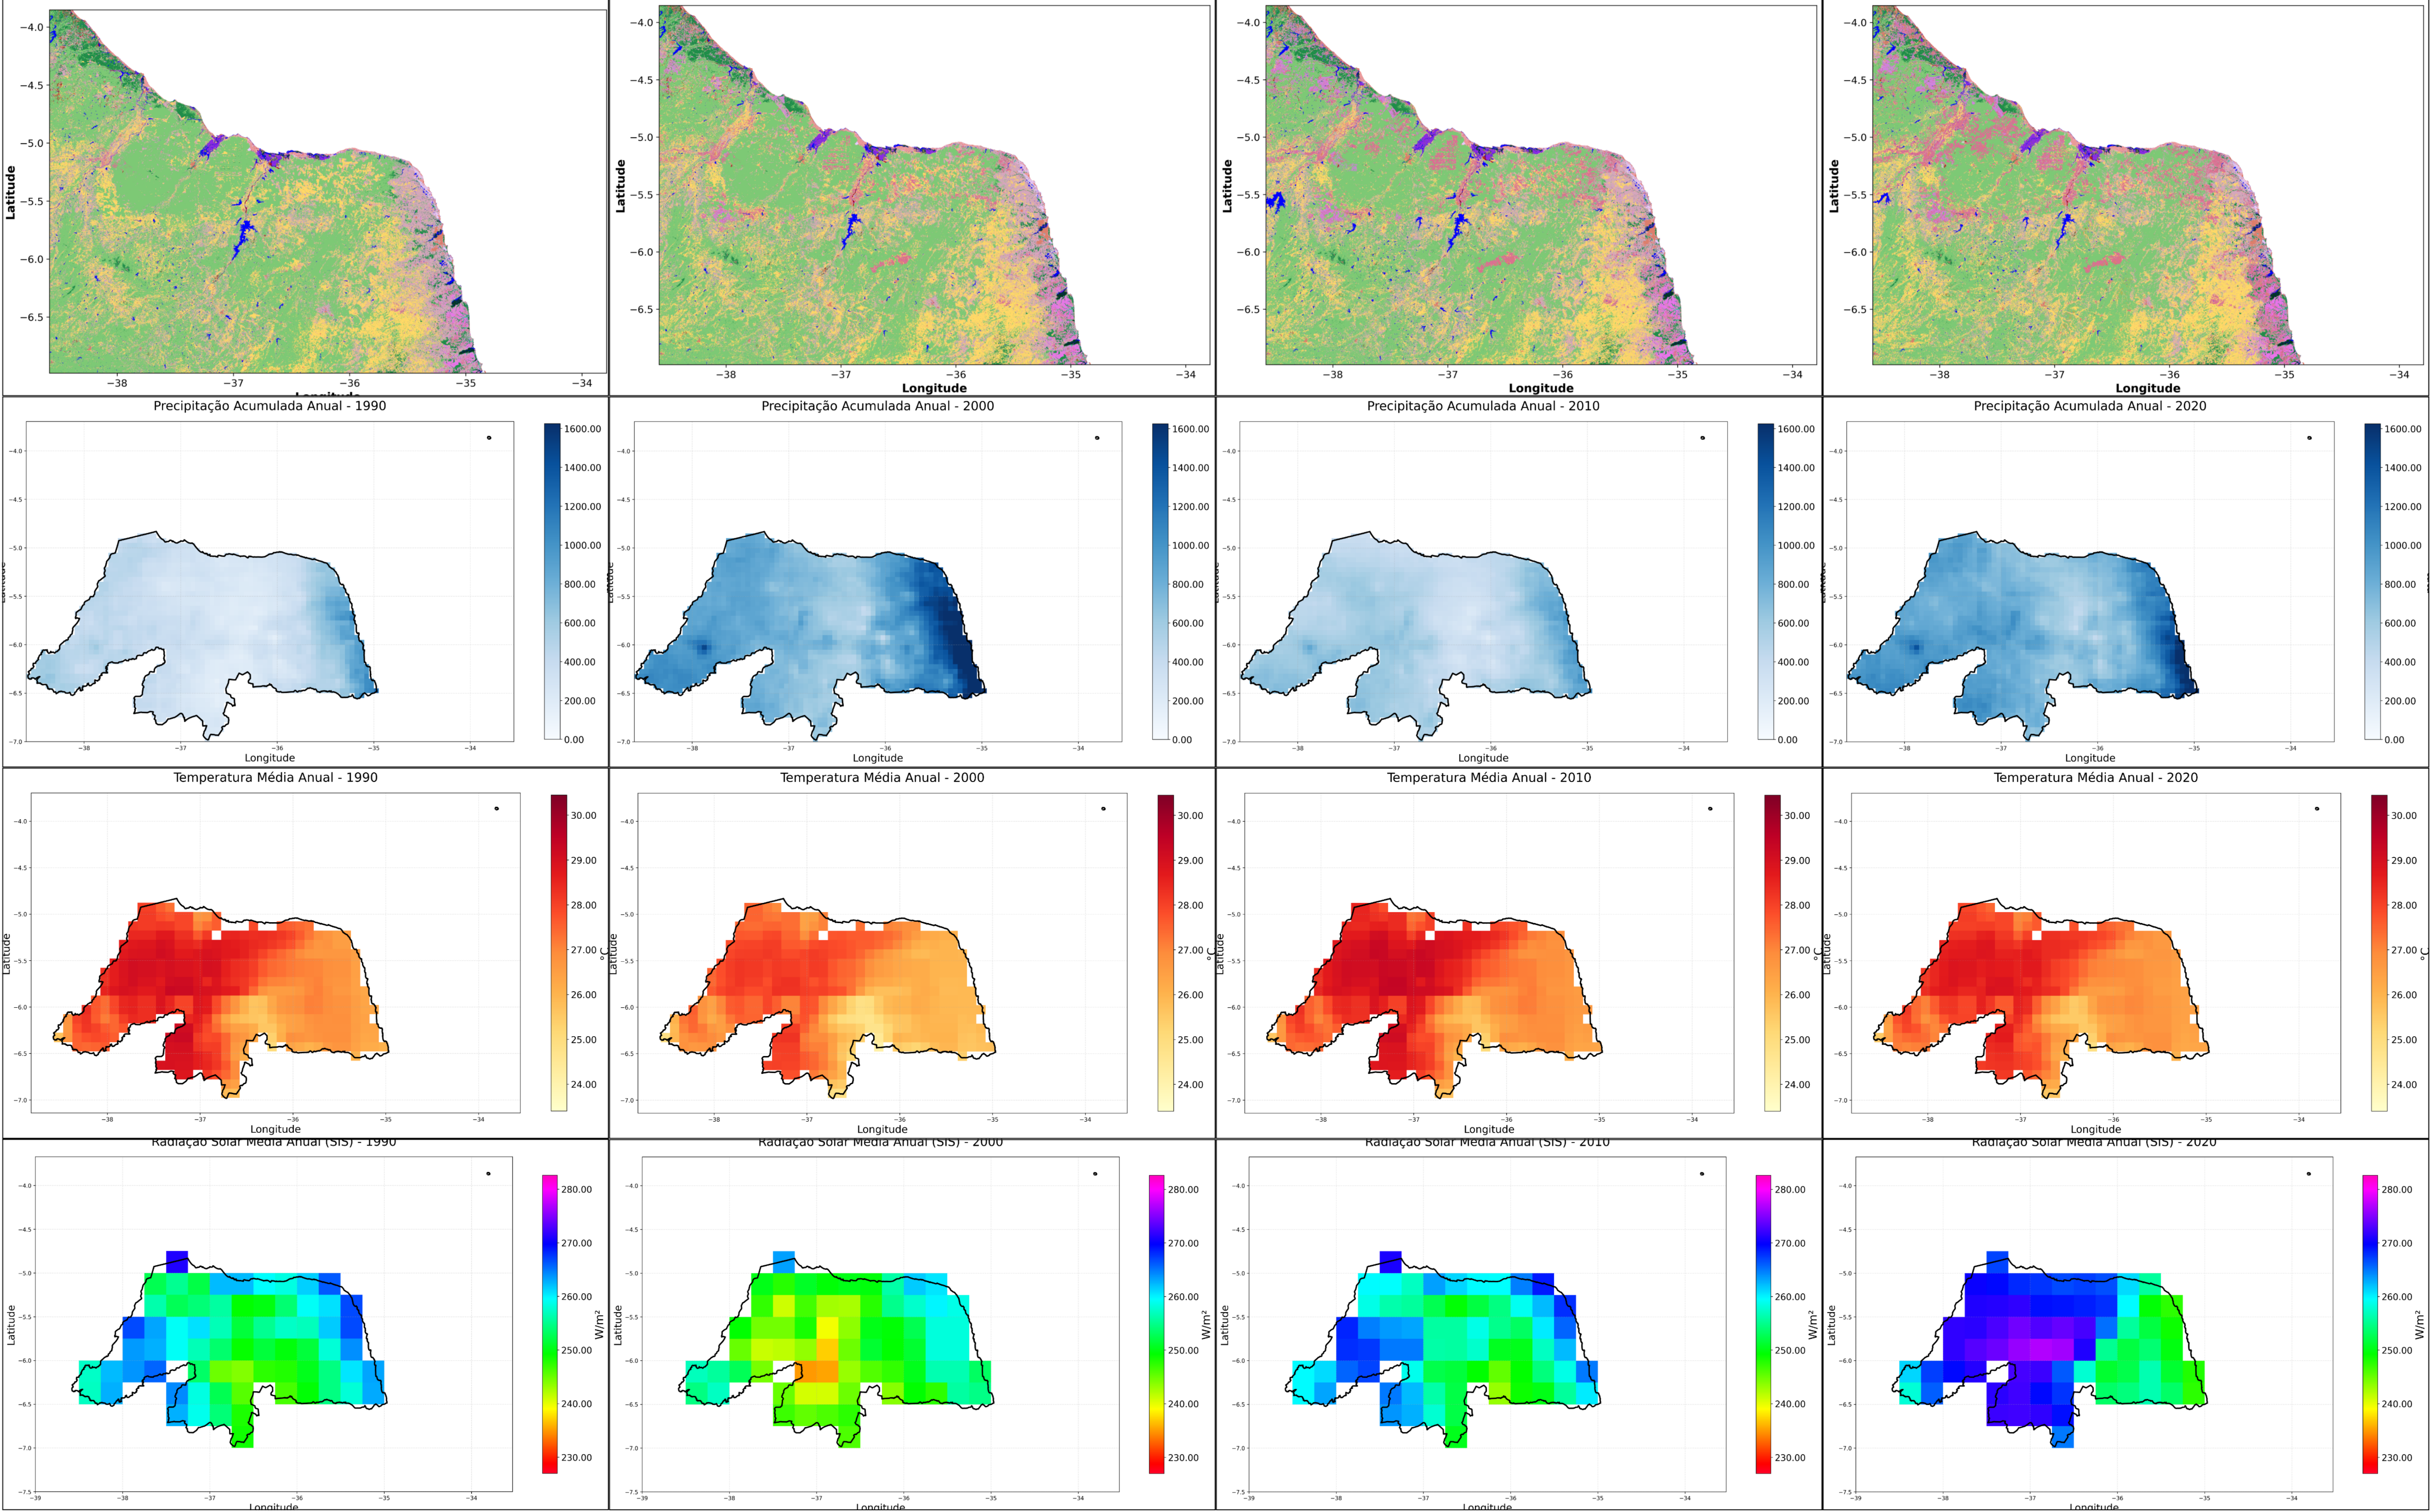
\includegraphics[width=\textwidth]{fig/mapas_rn.png}
	\caption[Evolução temporal do uso da terra - RN]{Evolução temporal do uso da terra (linha superior), precipitação acumulada anual (segunda linha), temperatura média anual (terceira linha) e radiação solar média anual (linha inferior) no Rio Grande do Norte para os anos de 1990, 2000, 2010 e 2020.}
	\label{fig:mapas_temporais_rn}
\end{figure}

A linha superior da Figura \ref{fig:mapas_temporais_rn} apresenta o processo de degradação progressiva e espacialmente heterogênea da Caatinga. Entre 1990 e 2020, observa-se conversão substancial de áreas verdes (Caatinga preservada) em tons amarelados e acastanhados (pastagens degradadas, solo exposto), particularmente intensa nas regiões centro-norte e central do estado.

As linhas de precipitação (segunda linha) e temperatura (terceira linha) não apresentam padrões espaciais de mudança claramente associados às áreas de maior degradação de Caatinga. A precipitação mantém gradiente leste-oeste característico (litoral úmido, interior seco) em todos os quatro períodos, com variações interanuais que refletem primariamente flutuações na intensidade da estação chuvosa ao invés de mudanças sistemáticas associadas a uso da terra.

A temperatura mostra gradiente norte-sul relativamente estável ao longo do período, com interior norte mais quente (27-28 °C) e litoral sul ligeiramente mais frio (26-27 °C). Não se identifica visualmente aquecimento localizado consistente em áreas que experimentaram maior degradação.

A radiação solar apresenta padrão espacial complexo que varia substancialmente entre os anos analisados, refletindo primariamente flutuações na nebulosidade durante a estação chuvosa. Não se observa aumento sistemático de radiação em áreas de maior degradação.


\section{Avaliação quantitativa sobre a influência da cobertura de superfície sobre variáveis climáticas}

Tomando como base os resultados anteriores que não evidenciavam claramente a influência da cobertura de superfície sobre as variáveis climáticas analisadas, adotou-se abordagem quantitativa mais refinada para investigar a relação entre diferentes tipos de cobertura da terra e as variáveis climáticas temperatura do ar, precipitação acumulada e radiação solar incidente na superfície. Esta análise considerou quatro classes distintas de cobertura segundo a classificação MapBiomas: Formação Florestal (Classe 3) para São Paulo, Formação Savânica (Classe 4) para Rio Grande do Norte, e Área Urbanizada (Classe 24) para ambos os estados, permitindo avaliar tanto o papel da vegetação nativa quanto o impacto da urbanização sobre o clima local.

A fundamentação teórica desta análise baseia-se no entendimento de que as modificações na cobertura da terra alteram o balanço de energia superficial através de múltiplos mecanismos biofísicos \citep{oke1982energetic}. A substituição de vegetação por superfícies impermeáveis modifica as propriedades radiativas (albedo), a rugosidade aerodinâmica, a capacidade de armazenamento térmico e os fluxos de calor latente e sensível \citep{arnfield2003two}. Em áreas urbanas, esses processos resultam no fenômeno conhecido como ilha de calor urbana (ICU), caracterizado por temperaturas significativamente mais elevadas nas cidades em comparação com áreas rurais adjacentes \citep{voogt2003thermal}.

\subsection{Abordagem metodológica}

A relação entre cobertura da terra e variáveis climáticas foi investigada por meio de regressão linear simples entre a fração percentual de cada classe de cobertura e as variáveis climáticas em cada ponto de grade espacial, seguindo metodologia análoga à empregada em estudos de sensibilidade climática à mudança de uso da terra \citep{li2015local, alkama2016biophysical}. O coeficiente angular ($\beta$) da regressão representa a sensibilidade da variável climática à variação da cobertura, sendo interpretado como a taxa média de mudança da variável climática por unidade percentual de cobertura. Valores positivos de $\beta$ indicam aumento da variável climática com o aumento da cobertura da classe analisada, enquanto valores negativos indicam relação inversa. Adicionalmente, calculou-se o percentual de pontos com relação estatisticamente significativa ($p < 0{,}05$), permitindo avaliar a robustez espacial das associações encontradas.

Esta abordagem permite distinguir entre correlações espúrias decorrentes de confundimento geográfico e relações potencialmente causais, uma vez que a análise ponto a ponto controla implicitamente fatores regionais de larga escala que poderiam confundir a interpretação dos resultados \citep{zhao2014strong}.

\subsection{Influência da Formação Florestal em São Paulo}

A análise da influência da Formação Florestal (Classe 3) sobre as variáveis climáticas no estado de São Paulo (Figura~\ref{fig:hist_beta_sp_classe3}) revela padrões distintos para cada variável.

\begin{figure}[H]
	\centering
	\includegraphics[width=1\textwidth]{fig/histograma_beta_influencia_cobertura_clima_sp_classe3.png}
	\caption[Distribuição dos coeficientes $\beta$ para Formação Florestal em São Paulo]{Distribuição dos coeficientes angulares ($\beta$) obtidos por regressão linear entre a fração de Formação Florestal (Classe 3) e as variáveis climáticas temperatura do ar, precipitação acumulada e radiação solar incidente, para o estado de São Paulo. A linha tracejada vertical indica $\beta = 0$.}
	\label{fig:hist_beta_sp_classe3}
\end{figure}

Para a temperatura, observa-se distribuição dos coeficientes $\beta$ ligeiramente deslocada para valores positivos, com mediana de $0{,}107$ °C/\% e média de $0{,}258$ °C/\%, sendo que $68{,}7\%$ dos pontos apresentaram relação estatisticamente significativa. Este resultado, aparentemente contraintuitivo uma vez que a literatura documenta consistentemente o efeito de resfriamento da vegetação através da evapotranspiração \citep{li2015local, alkama2016biophysical}, deve ser interpretado considerando o contexto geográfico específico do estado de São Paulo.

Os remanescentes de Formação Florestal em São Paulo concentram-se predominantemente na Serra do Mar e Serra da Mantiqueira, regiões caracterizadas por elevada altitude, alta nebulosidade orográfica e temperaturas naturalmente mais amenas devido ao gradiente adiabático. Assim, a correlação positiva observada reflete primariamente a distribuição geográfica das florestas remanescentes, que historicamente foram preservadas em áreas de topografia acidentada e difícil acesso agrícola, e não necessariamente um efeito causal da vegetação sobre a temperatura \citep{spracklen2018observations}. Estudos globais demonstram que, em regiões tropicais úmidas, florestas exercem efeito de resfriamento local da ordem de 0,5 a 2,0 °C através do aumento da evapotranspiração \citep{li2015local}.

Para a precipitação, a distribuição apresenta-se centrada próxima a zero com ligeira assimetria negativa ($\beta_{\text{mediana}} = -5{,}01$ mm/\%), porém com apenas $7{,}3\%$ dos pontos apresentando significância estatística. Este resultado indica que a relação entre cobertura florestal e precipitação é fraca e espacialmente inconsistente no contexto paulista. Embora estudos regionais na Amazônia demonstrem contribuição significativa da evapotranspiração florestal para a precipitação através da reciclagem de umidade atmosférica \citep{spracklen2012observations, staal2018forest}, no contexto de São Paulo, onde os remanescentes florestais são fragmentados e representam fração relativamente pequena da cobertura total, este mecanismo provavelmente não é dominante.

A radiação solar apresenta distribuição com predominância de valores positivos ($\beta_{\text{mediana}} = 1{,}09$ W/m$^2$/\%), com $55{,}2\%$ dos pontos significativos. Este padrão reflete novamente a distribuição geográfica das florestas na Serra do Mar, região caracterizada por nebulosidade orográfica persistente. A maior incidência de radiação em áreas florestadas, neste contexto, resulta da localização das mesmas em vertentes com orientação favorável à insolação, e não de um efeito direto da vegetação sobre a radiação incidente.

\subsection{Influência da Área Urbanizada em São Paulo}

Em contraste marcante com a Formação Florestal, a análise da influência da Área Urbanizada (Classe 24) em São Paulo (Figura~\ref{fig:hist_beta_sp_classe24}) revela relações substancialmente mais intensas e estatisticamente claras, particularmente para temperatura e radiação solar. Estes resultados são consistentes literaturas que destacam o fenômeno de ilha de calor urbana \citep{oke1982energetic, arnfield2003two, voogt2003thermal}.

\begin{figure}[H]
	\centering
	\includegraphics[width=1\textwidth]{fig/histograma_beta_influencia_cobertura_clima_sp_classe24.png}
	\caption[Distribuição dos coeficientes $\beta$ para Área Urbanizada em São Paulo]{Distribuição dos coeficientes angulares ($\beta$) obtidos por regressão linear entre a fração de Área Urbanizada (Classe 24) e as variáveis climáticas temperatura do ar, precipitação acumulada e radiação solar incidente, para o estado de São Paulo. Observe a forte assimetria positiva para temperatura e radiação.}
	\label{fig:hist_beta_sp_classe24}
\end{figure}

A temperatura apresenta relação positiva forte e consistente com a formação urbana, com $\beta_{\text{mediana}} = 0{,}97$ °C/\% e $\beta_{\text{média}} = 4{,}75$ °C/\%. Notavelmente, $93{,}8\%$ dos pontos analisados apresentaram relação estatisticamente significativa, configurando o resultado mais adequado de toda a análise. A magnitude desta sensibilidade é comparável aos valores reportados em estudos globais, que documentam intensidades de ilha de calor urbana variando tipicamente entre 1 e 7 °C durante o dia e 2 a 5 °C durante a noite \citep{imhoff2010remote, peng2012surface, zhao2014strong}.

O mecanismo físico subjacente a este aquecimento urbano está bem estabelecido na literatura \citep{oke1982energetic, arnfield2003two}. A substituição de vegetação por superfícies impermeáveis (asfalto, concreto, edificações) resulta casos como: (i) redução da evapotranspiração e consequente diminuição do fluxo de calor latente, com maior partição da energia disponível para aquecimento sensível; (ii) aumento da capacidade de armazenamento térmico das superfícies urbanas, que absorvem calor durante o dia e o liberam gradualmente à noite e (iii) redução do albedo em algumas configurações urbanas, aumentando a absorção de radiação solar \citep{sailor2011review}.

Estudos específicos para a Região Metropolitana de São Paulo corroboram estes resultados, documentando intensidades de ilha de calor de 5 a 10 °C entre áreas centrais densamente urbanizadas e periferias mais vegetadas \citep{ferreira2019urban, santos2017assessment}. A elevada significância estatística observada ($93{,}8\%$) indica que este fenômeno é espacialmente consistente.

A radiação solar também apresenta relação positiva pronunciada ($\beta_{\text{mediana}} = 11{,}99$ W/m$^2$/\%), com $75{,}3\%$ dos pontos significativos. Este resultado indica que áreas mais urbanizadas tendem a receber maior radiação solar na superfície, fenômeno que pode ser atribuído a múltiplos mecanismos. Primeiro, a redução da cobertura vegetal diminui a formação de nuvens convectivas rasas associadas à evapotranspiração, aumentando a transmissividade atmosférica \citep{teuling2017contrasting}. Segundo, a geometria urbana com edificações altas e ruas estreitas pode criar microclimas com maior exposição solar em determinados horários. Terceiro, a concentração de aerossóis urbanos pode ter efeitos complexos e não-lineares sobre a radiação, dependendo da composição e concentração específicas \citep{li2016aerosol}.

Para a precipitação, observa-se tendência negativa ($\beta_{\text{mediana}} = -35{,}64$ mm/\%), sugerindo que a urbanização pode estar associada à redução da precipitação local, embora apenas $10{,}1\%$ dos pontos apresentem significância estatística. A literatura sobre efeitos urbanos na precipitação é substancialmente mais controversa que aquela sobre temperatura \citep{shepherd2005review, niyogi2017urbanization}. Estudos clássicos do projeto METROMEX documentaram aumento de precipitação a sotavento de cidades norte-americanas \citep{changnon1981metromex}, enquanto trabalhos mais recentes sugerem que o efeito pode ser altamente dependente do contexto climático regional e das características específicas da área urbana \citep{han2014effects, liu2017precipitation}.

A tendência negativa observada em São Paulo pode refletir a redução da reciclagem local de umidade devido à diminuição da evapotranspiração em áreas impermeabilizadas. Estudos recentes utilizando dados de satélite em escala global encontraram padrões assimétricos, com aumento de eventos de baixa intensidade e redução de eventos de alta intensidade sobre áreas urbanas \citep{li2020asymmetric}, o que poderia resultar em balanço negativo quando considerados acumulados totais.

\subsection{Influência da Formação Savânica no Rio Grande do Norte}

A análise da Formação Savânica (Caatinga, Classe 4) no Rio Grande do Norte (Figura~\ref{fig:hist_beta_rn_classe4}) revela padrões substancialmente distintos daqueles observados em São Paulo, com relações predominantemente fracas e centradas em torno de zero para todas as variáveis climáticas.

\begin{figure}[H]
	\centering
	\includegraphics[width=1\textwidth]{fig/histograma_beta_influencia_cobertura_clima_rn_classe4.png}
	\caption[Distribuição dos coeficientes $\beta$ para Formação Savânica no Rio Grande do Norte]{Distribuição dos coeficientes angulares ($\beta$) obtidos por regressão linear entre a fração de Formação Savânica (Classe 4) e as variáveis climáticas no Rio Grande do Norte. Observe as distribuições aproximadamente simétricas e centradas próximas a zero.}
	\label{fig:hist_beta_rn_classe4}
\end{figure}

Para a temperatura, a distribuição é notavelmente simétrica e centrada em zero ($\beta_{\text{mediana}} = -0{,}0024$ °C/\%), com apenas $0{,}56\%$ dos pontos apresentando significância estatística. Este resultado indica ausência de relação detectável entre cobertura de Caatinga e temperatura local, contrastando fortemente com o efeito de resfriamento documentado para florestas tropicais úmidas \citep{li2015local, alkama2016biophysical}.

A explicação para esta ausência de sinal reside nas características ecofisiológicas específicas da vegetação de Caatinga e nas condições climáticas do semiárido. Estudos recentes sobre o papel termorregulador da vegetação em regiões áridas e semiáridas demonstram que o efeito de resfriamento por evapotranspiração é substancialmente reduzido ou mesmo revertido quando a disponibilidade hídrica é limitante \citep{shen2015dryland, duveiller2018local}. Em condições de déficit hídrico severo, características da maior parte do ano no semiárido nordestino, a vegetação de Caatinga adota estratégias de conservação de água, incluindo fechamento estomático e abscisão foliar, que minimizam a transpiração e consequentemente o efeito de resfriamento evaporativo.

A elevada variabilidade climática interanual característica do semiárido nordestino também contribui para mascarar possíveis relações entre cobertura vegetal e temperatura. O coeficiente de variação da precipitação anual no semiárido frequentemente excede 40-50\%, com secas plurianuais alternando com períodos de chuvas abundantes em escalas decadais \citep{marengo2017drought}. Esta variabilidade climática natural domina completamente sobre possíveis sinais associados à mudança de cobertura vegetal, particularmente em séries temporais de três décadas como as utilizadas neste estudo.

A precipitação apresenta ligeira tendência negativa ($\beta_{\text{mediana}} = -6{,}32$ mm/\%), com $9{,}8\%$ dos pontos significativos. Embora este resultado possa sugerir contribuição da vegetação para a precipitação através de reciclagem de umidade, a baixa significância estatística impede conclusões definitivas. Estudos sobre o papel da vegetação na precipitação em regiões semiáridas são escassos e apresentam resultados contraditórios \citep{sheil2018forest, staal2018forest}, em parte porque os mecanismos de retroalimentação vegetação-precipitação são mais fracos em ambientes com déficit hídrico crônico.

A radiação solar mostra distribuição praticamente centrada em zero ($\beta_{\text{mediana}} = -0{,}09$ W/m$^2$/\%), embora com $39{,}5\%$ dos pontos significativos. A maior significância relativa para radiação pode refletir o papel da nebulosidade durante a estação chuvosa, que covaria espacialmente com a densidade de vegetação preservada.

\subsection{Influência da Área Urbanizada no Rio Grande do Norte}

A análise da Área Urbanizada (Classe 24) no Rio Grande do Norte (Figura~\ref{fig:hist_beta_rn_classe24}) apresenta padrões intermediários entre a Formação Savânica local e a urbanização paulista, revelando aspectos importantes sobre a modulação do efeito de ilha de calor urbana pelo contexto climático regional.

\begin{figure}[H]
	\centering
	\includegraphics[width=1\textwidth]{fig/histograma_beta_influencia_cobertura_clima_rn_classe24.png}
	\caption[Distribuição dos coeficientes $\beta$ para Área Urbanizada no Rio Grande do Norte]{Distribuição dos coeficientes angulares ($\beta$) obtidos por regressão linear entre a fração de Área Urbanizada (Classe 24) e as variáveis climáticas no Rio Grande do Norte.}
	\label{fig:hist_beta_rn_classe24}
\end{figure}

A temperatura apresenta relação positiva fraca ($\beta_{\text{mediana}} = 0{,}072$ °C/\%), porém com apenas $2{,}0\%$ dos pontos significativos. Este resultado contrasta marcadamente com a forte significância observada em São Paulo ($93{,}8\%$). A literatura recente sobre ilhas de calor em climas secos sugere que a intensidade do fenômeno depende criticamente do contraste entre evapotranspiração urbana e rural \citep{zhao2014strong, manoli2019magnitude}. Em regiões onde a vegetação rural já apresenta baixa evapotranspiração devido à limitação hídrica, como no semiárido nordestino, o diferencial térmico urbano-rural é naturalmente atenuado.

Estudos globais demonstram que a intensidade de ilha de calor urbana é inversamente correlacionada com a aridez do entorno rural \citep{manoli2019magnitude}. Em cidades localizadas em climas úmidos, onde a vegetação rural transpira ativamente e resfria o ar circundante, a substituição desta vegetação por superfícies impermeáveis resulta em forte aquecimento. Em contraste, em cidades de climas áridos e semiáridos, onde a vegetação rural já está sob estresse hídrico e apresenta baixa evapotranspiração, o contraste urbano-rural é menos pronunciado \citep{liao2018stronger}.

Resultado particularmente interessante emerge para a precipitação, que apresenta relação positiva ($\beta_{\text{mediana}} = 194{,}83$ mm/\%, $\beta_{\text{média}} = 889{,}97$ mm/\%), embora com baixa significância estatística ($2{,}9\%$). Este padrão, oposto ao observado em São Paulo, pode estar associado ao fenômeno de intensificação da convecção urbana em ambientes semiáridos.

O mecanismo físico proposto baseia-se no aquecimento diferencial entre superfícies urbanas e rurais. Em cidades de clima seco, o efeito de ilha de calor pode criar gradientes térmicos horizontais significativos que induzem circulações locais de mesoescala \citep{shepherd2005review}. Estas circulações, caracterizadas por convergência de ar na camada limite sobre a área urbana, podem favorecer o disparo de convecção e a formação de precipitação, particularmente durante períodos transicionais quando há umidade atmosférica disponível \citep{niyogi2017urbanization}. Este mecanismo foi documentado em estudos de caso em cidades de clima tropical e subtropical, incluindo Atlanta, Houston e cidades mexicanas \citep{shepherd2002atlanta, jauregui1996urban}.

A radiação solar apresenta relação positiva moderada ($\beta_{\text{mediana}} = 3{,}73$ W/m$^2$/\%), com $59{,}9\%$ dos pontos significativos. Este resultado é consistente com a hipótese de que áreas urbanizadas no semiárido apresentam menor formação de nuvens convectivas devido à supressão da evapotranspiração, resultando em maior transmissividade atmosférica e incidência de radiação solar na superfície.

\subsection{Síntese estatística comparativa}

A Tabela~\ref{tab:beta_cobertura_clima_completa} sintetiza os resultados estatísticos para todas as classes e estados analisados.

\begin{table}[H]
	\centering
	\caption{Estatísticas dos coeficientes de regressão ($\beta$) entre cobertura da terra e variáveis climáticas para diferentes classes de uso em São Paulo (SP) e Rio Grande do Norte (RN).}
	\label{tab:beta_cobertura_clima_completa}
	\small
	\begin{tabular}{llccccc}
		\hline
		\textbf{Estado} & \textbf{Classe} & \textbf{Variável} & $N$ & $\beta_{\text{med}}$ & $\beta_{\text{média}}$ & \textbf{\% Signif.} \\
		\hline
		SP & Florestal (3) & Temperatura & 3605 & 0,107 & 0,258 & 68,7 \\
		SP & Florestal (3) & Precipitação & 3605 & $-$5,01 & $-$56,69 & 7,3 \\
		SP & Florestal (3) & Radiação & 3605 & 1,09 & 2,22 & 55,2 \\
		\hline
		SP & Urbanizada (24) & Temperatura & 1216 & 0,97 & 4,75 & \textbf{93,8} \\
		SP & Urbanizada (24) & Precipitação & 1216 & $-$35,64 & $-$478,76 & 10,1 \\
		SP & Urbanizada (24) & Radiação & 1216 & 11,99 & 58,45 & 75,3 \\
		\hline
		RN & Savânica (4) & Temperatura & 1416 & $-$0,002 & $-$0,009 & 0,6 \\
		RN & Savânica (4) & Precipitação & 1416 & $-$6,32 & $-$19,12 & 9,8 \\
		RN & Savânica (4) & Radiação & 1416 & $-$0,09 & 0,19 & 39,5 \\
		\hline
		RN & Urbanizada (24) & Temperatura & 653 & 0,072 & 0,919 & 2,0 \\
		RN & Urbanizada (24) & Precipitação & 653 & 194,83 & 889,97 & 2,9 \\
		RN & Urbanizada (24) & Radiação & 653 & 3,73 & 26,20 & 59,9 \\
		\hline
	\end{tabular}
	
	\vspace{2mm}
	{\footnotesize
		$N$ = número de pontos espaciais; $\beta_{\text{med}}$ = mediana; \% Signif. = percentual de pontos com $p < 0{,}05$.}
\end{table}

Os resultados desta análise revelam que a influência da cobertura da terra sobre as variáveis climáticas é fortemente condicionada tanto pelo tipo de cobertura quanto pelo contexto climático regional.

\subsubsection*{Urbanização como principal forçante climática antrópica detectável}

A urbanização apresenta impacto climático substancialmente mais intenso e estatisticamente consitênte que as formações vegetais nativas. Em São Paulo, a relação entre área urbanizada e temperatura ($93{,}8\%$ de significância, $\beta_{\text{mediana}} = 0{,}97$ °C/\%) constitui o resultado mais considerável de toda a análise, configurando evidência consistente do fenômeno de ilha de calor urbana \citep{oke1982energetic, arnfield2003two, peng2012surface}.

A magnitude do efeito observado ($\approx 1$ °C por ponto percentual de urbanização) implica que, em áreas com urbanização intensa (30-50\% de cobertura urbana), o aquecimento local atribuível à urbanização pode alcançar 3-5 °C, valor comparável ou superior às tendências de aquecimento climático de longo prazo documentadas nas seções anteriores deste trabalho. Este resultado corrobora estudos recentes que demonstram que, em escala local, os efeitos da urbanização sobre a temperatura podem igualar ou exceder os efeitos das mudanças climáticas globais \citep{zhao2014strong, heaviside2017physical}.

\subsubsection*{Modulação do efeito de ilha de calor pelo contexto climático}

O contexto climático regional modula fortemente a detectabilidade dos efeitos da urbanização. Enquanto em São Paulo $93{,}8\%$ dos pontos apresentaram relação significativa entre urbanização e temperatura, no Rio Grande do Norte apenas $2{,}0\%$ alcançaram significância. Esta diferença de quase 50 vezes na detectabilidade do fenômeno não pode ser atribuída simplesmente a diferenças no tamanho amostral ou intensidade de urbanização, mas reflete mecanismos biofísicos fundamentais.

Conforme demonstrado por \cite{zhao2014strong} e \cite{manoli2019magnitude} em análises globais, a intensidade de ilha de calor urbana depende criticamente do contraste de evapotranspiração entre áreas urbanas e rurais. Em climas úmidos, a vegetação rural transpira ativamente e resfria o ar circundante através da conversão de energia radiativa em calor latente. A substituição desta vegetação por superfícies impermeáveis resulta em forte aquecimento porque elimina este mecanismo de resfriamento. Em contraste, em climas secos e semiáridos, a vegetação rural já está sob estresse hídrico e apresenta evapotranspiração limitada, reduzindo o diferencial térmico potencial entre áreas urbanas e rurais.

\subsubsection*{Limitações na detecção de efeitos da vegetação nativa}

A ausência de relação detectável entre cobertura de Caatinga e temperatura no Rio Grande do Norte (apenas $0{,}6\%$ de significância) contrasta com a literatura que documenta efeitos de resfriamento da vegetação em escala global \citep{li2015local, alkama2016biophysical}. Esta aparente contradição pode ser explicada por três fatores complementares.

Primeiro, os estudos globais que documentam resfriamento por vegetação baseiam-se predominantemente em comparações entre florestas e áreas agrícolas ou pastagens em regiões úmidas, onde a vegetação apresenta evapotranspiração ativa durante a maior parte do ano. A Caatinga, como vegetação adaptada a condições semiáridas com déficit hídrico severo durante 8-9 meses do ano, apresenta estratégias ecofisiológicas que minimizam a transpiração e consequentemente o efeito de resfriamento evaporativo \citep{santos2014caatinga}.

Segundo, a elevada variabilidade climática interanual do semiárido nordestino, com coeficientes de variação de precipitação frequentemente excedendo 40-50\%, introduz ``ruído'' substancial nas séries temporais que mascara possíveis sinais de menor magnitude associados à mudança de cobertura vegetal \citep{marengo2017drought}.

Terceiro, a escala temporal da análise (dados anuais agregados) pode ser inadequada para capturar efeitos que se manifestam primariamente em escalas sazonais ou diurnas. Estudos de processo indicam que o efeito de resfriamento da vegetação é máximo durante o período de transpiração ativa (estação chuvosa na Caatinga) e durante as horas de máxima insolação \citep{duveiller2018local}. Análises com resolução temporal mais fina poderiam revelar padrões não detectáveis em médias anuais.

\subsubsection*{Diferenças qualitativas na resposta da precipitação à urbanização}

As diferenças observadas na resposta da precipitação à urbanização entre São Paulo (tendência negativa, $\beta_{\text{mediana}} = -35{,}64$ mm/\%) e Rio Grande do Norte (tendência positiva, $\beta_{\text{mediana}} = +194{,}83$ mm/\%) sugerem mecanismos físicos distintos operando nos dois contextos climáticos.

A literatura sobre efeitos urbanos na precipitação é substancialmente mais controversa que aquela sobre temperatura \citep{shepherd2005review, han2014effects, niyogi2017urbanization}. Estudos sugerem que a urbanização pode tanto aumentar quanto diminuir a precipitação local, dependendo de fatores como localização geográfica, regime climático dominante, tamanho e morfologia da área urbana, e características dos sistemas precipitantes \citep{liu2017precipitation}.

Em São Paulo, a tendência negativa pode refletir a redução da reciclagem local de umidade devido à diminuição da evapotranspiração em áreas impermeabilizadas. Este mecanismo é consistente com estudos que demonstram redução de precipitação sobre e a sotavento de áreas urbanas em contextos onde a reciclagem de umidade local é importante para a precipitação total \citep{spracklen2012observations}.

No Rio Grande do Norte, a tendência positiva pode resultar da intensificação da convecção urbana em ambiente semiárido. O aquecimento diferencial entre superfícies urbanas e rurais cria gradientes térmicos horizontais que induzem convergência de ar na camada limite urbana, favorecendo o disparo de convecção quando há umidade atmosférica disponível \citep{shepherd2002atlanta, niyogi2017urbanization}. Este mecanismo pode ser particularmente relevante durante a estação chuvosa do semiárido, quando a combinação de umidade atmosférica elevada e aquecimento superficial intenso cria condições favoráveis à convecção profunda.	
